\documentclass[10pt,letterpaper]{article}
% Built by split_appendix.py from evidence_appendix.tex (build.py, ../results/*.json). Needs only texlive-latex-base.
\usepackage[T1]{fontenc}
\usepackage[utf8]{inputenc}
\usepackage{lmodern}
\usepackage{textcomp}
\usepackage[margin=1in]{geometry}
\usepackage{amsmath,amssymb}
\usepackage{graphicx}
\usepackage{array,tabularx,longtable}
\usepackage{url}
\IfFileExists{etoolbox.sty}{\usepackage[hidelinks]{hyperref}}{}
\newcommand{\doclink}[2]{\ifdefined\href\href{#1}{#2}\else#2\fi}
\usepackage{fancyhdr}

% Characters that appear in data-driven text
\DeclareUnicodeCharacter{2192}{\ensuremath{\rightarrow}}
\DeclareUnicodeCharacter{2190}{\ensuremath{\leftarrow}}
\DeclareUnicodeCharacter{2264}{\ensuremath{\le}}
\DeclareUnicodeCharacter{2265}{\ensuremath{\ge}}
\DeclareUnicodeCharacter{2212}{\ensuremath{-}}
\DeclareUnicodeCharacter{2248}{\ensuremath{\approx}}
\DeclareUnicodeCharacter{0394}{\ensuremath{\Delta}}
\DeclareUnicodeCharacter{2032}{\ensuremath{'}}
\DeclareUnicodeCharacter{220F}{\ensuremath{\prod}}
\DeclareUnicodeCharacter{207B}{\ensuremath{^{-}}}
\DeclareUnicodeCharacter{2070}{\ensuremath{^{0}}}
\DeclareUnicodeCharacter{00B9}{\ensuremath{^{1}}}
\DeclareUnicodeCharacter{2074}{\ensuremath{^{4}}}
\DeclareUnicodeCharacter{2075}{\ensuremath{^{5}}}
\DeclareUnicodeCharacter{2080}{\ensuremath{_{0}}}
\DeclareUnicodeCharacter{1D62}{\ensuremath{_{i}}}
\DeclareUnicodeCharacter{00B2}{\ensuremath{^{2}}}
\DeclareUnicodeCharacter{00B3}{\ensuremath{^{3}}}
\DeclareUnicodeCharacter{2076}{\ensuremath{^{6}}}
\DeclareUnicodeCharacter{2077}{\ensuremath{^{7}}}
\DeclareUnicodeCharacter{2078}{\ensuremath{^{8}}}
\DeclareUnicodeCharacter{2079}{\ensuremath{^{9}}}
\DeclareUnicodeCharacter{2081}{\ensuremath{_{1}}}
\DeclareUnicodeCharacter{2082}{\ensuremath{_{2}}}
\DeclareUnicodeCharacter{2083}{\ensuremath{_{3}}}
\DeclareUnicodeCharacter{2084}{\ensuremath{_{4}}}
\DeclareUnicodeCharacter{2085}{\ensuremath{_{5}}}
\DeclareUnicodeCharacter{2086}{\ensuremath{_{6}}}
\DeclareUnicodeCharacter{2087}{\ensuremath{_{7}}}
\DeclareUnicodeCharacter{2088}{\ensuremath{_{8}}}
\DeclareUnicodeCharacter{2089}{\ensuremath{_{9}}}

\setlength{\extrarowheight}{0.5pt}
\newcolumntype{L}{>{\raggedright\arraybackslash}X}
\newcolumntype{R}{>{\raggedleft\arraybackslash}X}
\setlength{\parskip}{2pt plus 1pt}
\setlength{\parindent}{0pt}
\setlength{\textfloatsep}{8pt plus 2pt minus 2pt}
\setlength{\floatsep}{8pt plus 2pt minus 2pt}
\setlength{\intextsep}{8pt plus 2pt minus 2pt}
\setlength{\abovecaptionskip}{3pt}
\setlength{\belowcaptionskip}{3pt}
\renewcommand{\topfraction}{0.9}
\renewcommand{\bottomfraction}{0.8}
\renewcommand{\textfraction}{0.07}
\renewcommand{\floatpagefraction}{0.85}
\setcounter{topnumber}{3}
\setcounter{bottomnumber}{2}
\setcounter{totalnumber}{4}
\setlength{\LTpre}{4pt}
\setlength{\LTpost}{4pt}
\AtBeginDocument{\setlength{\LTcapwidth}{\textwidth}}
\makeatletter
% compact section headings
\renewcommand\section{\@startsection{section}{1}{\z@}{-9pt plus -2pt minus -1pt}{3pt}{\normalfont\large\bfseries}}
\renewcommand\subsection{\@startsection{subsection}{2}{\z@}{-6pt plus -2pt minus -1pt}{2pt}{\normalfont\normalsize\bfseries}}
\renewcommand\paragraph{\@startsection{paragraph}{4}{\z@}{4pt plus 1pt}{-0.6em}{\normalfont\normalsize\bfseries}}
\makeatother
\pagestyle{plain}
\newcommand{\tablefont}{\normalsize}
\begin{document}
\begin{center}{\LARGE\bfseries Evidence Appendix: Supplement\par}\end{center}

\linespread{0.95}\selectfont
\renewcommand{\thetable}{B\arabic{table}}\renewcommand{\thefigure}{B\arabic{figure}}
\section*{About this supplement}
This supplement to the evidence appendix (\texttt{appendix\_short.pdf}) holds the detail behind it: complete traces,
every launch and every ledger change. Its tables are numbered B; tables numbered A are in the appendix. Every result
comes from the same simulator runs as the appendix, and the machine-readable traces are in
\texttt{milestone2/traces/}.

\section*{F. Message formats and sizes}
Every message has a fixed-width binary layout. The tables below give every field, and the record sizes are the
ones the simulator uses for packing. Integers are unsigned big-endian unless a field says otherwise. Times are signed
64-bit integer milliseconds of TDB since the epoch. Money is in integer cents, and share quantities are whole shares.
Each record carries the signature of the principal that issued it, so it can be checked at any exchange whatever
session or forwarder carried it.

\begin{table}[!htb]\centering\tablefont\setlength{\tabcolsep}{4pt}
\caption{Common header of every application record.}\label{tab:fcommon}
\begin{tabularx}{\linewidth}{@{}lL@{}}\noalign{\vskip 1pt}\hline\noalign{\vskip 1pt}\textbf{Field} & \textbf{Bytes and meaning} \\\hline\noalign{\vskip 1pt}
Type & 1: Record type code \\
Version & 1: Format version (1) \\
Length & 2: Record length in bytes \\
Record ID & 12: 32-bit principal prefix and 64-bit counter; never reused \\
Created & 8: Signed 64-bit integer milliseconds of TDB since the epoch \\
Signature & 64: Ed25519 by the issuing principal over every other byte of the record \\
Total & 88 \\\noalign{\vskip 1pt}\hline
\end{tabularx}
\end{table}
\begin{table}[!htb]\centering\tablefont\setlength{\tabcolsep}{3pt}
\caption{Fixed-width body of each record type. The totals are the sizes the simulator charges (\texttt{protocol.SIZE}); the build checks that the fields add up to them. A STATUS record grows by 16 bytes for each entry after the first.}\label{tab:fbody}
\begin{tabularx}{\linewidth}{@{}lrL@{}}\noalign{\vskip 1pt}\hline\noalign{\vskip 1pt}\textbf{Record} & \textbf{Bytes} & \textbf{Fields after the common header (bytes)} \\\hline\noalign{\vskip 1pt}
TRANSFER & 176 & Source exchange 1; Destination exchange 1; Purpose 1; Asset 1; Owner account 8; Amount (units or cents) 8; Number n to this destination 8; Reference ID (order, contract, request) 12; Beneficiary account 8; Terms digest (SHA-256) 32; Reserved 8 \\
RECEIVED & 120 & Transfer ID 12; Source exchange 1; Result (credited, restricted) 1; Import time 8; Watermark W for this source 8; Reserved 2 \\
ORDER & 128 & Account 8; Host 1; Asset 1; Side 1; Time in force 1; Quantity 8; Limit price (cents) 8; Expiry 8; Disposition (keep, home) 1; Reserved 3 \\
CANCEL & 128 & Account 8; Target order ID 12; Reserved 20 \\
WITHDRAW & 128 & Account 8; Asset 1; Destination exchange 1; Amount 8; Reserved 22 \\
CLOSE & 128 & Account 8; Reserved 32 \\
CINSTR & 256 & Account 8; Contract ID 12; Role (long, short) 1; Quantity Q 8; Multiplier 4; Opening price K 8; Floor 8; Cap 8; Five observation times 40; Maturity 8; Fixing time 8; Opening deadline 8; Counterparty account 8; Price source 8; Margin 8; Reserved 23 \\
STATUS & 128 & Host exchange 1; Home exchange 1; Entry count m (1 to 52) 2; As-of time 8; Reserved 12; Entry 1: account 8, contract counter 6, state 1, flags 1 16 \\
PRICE & 200 & Contract ID 12; Observation number 1; Index value (fixed point) 8; Observation time 8; Price source 8; Source attestation (Ed25519) 64; Reserved 11 \\
MDS & 152 & Market exchange 1; Asset 1; Book version 8; Best bid (cents) 8; Bid size 4; Best ask (cents) 8; Ask size 4; Last trade price (cents) 8; Last trade size 4; Last trade time 8; Reserved 10 \\
MDREQ & 120 & Requesting exchange 1; Asset 1; Reserved 30 \\\noalign{\vskip 1pt}\hline
\end{tabularx}
\end{table}
\begin{table}[!htb]\centering\tablefont\setlength{\tabcolsep}{3pt}
\caption{Packet layouts. Every packet is at most 1,024 bytes: the brief's 64-byte header and at most 960 bytes of payload.}\label{tab:fpkt}
\begin{tabularx}{\linewidth}{@{}llL@{}}\noalign{\vskip 1pt}\hline\noalign{\vskip 1pt}\textbf{Unit} & \textbf{Bytes} & \textbf{Layout} \\\hline\noalign{\vskip 1pt}
Network header (brief) & 64 & Every packet; defined by the network \\
Data sub-header & 16 & Session 8, data sequence 4, record count 2, flags 2 \\
Data packet & 64 + 16 + records & Whole records, at most 944 bytes of records \\
SYN, SYN-ACK, ACK, DACK payload & 96 & Session 8, route 4, data sequence 4, attempt 1, kind 1, reserved 6, time 8, signature 64 \\
Hop receipt payload & 16 & Packet ID 12, launch number 1, reserved 3 \\
Direct sub-header & 16 & Principal 8, packet sequence 4, instruction count 1, flags 1, reserved 2 \\
Direct packet & 64 + 16 + instructions & Whole signed instructions, at most 944 bytes \\
FWD wrapper (R8) & 24 + inner & Forwarder 1, target host 1, attempt 1, flags 1, forward time 8, origin principal 8, inner length 2, reserved 2 \\\noalign{\vskip 1pt}\hline
\end{tabularx}
\end{table}
\begin{table}[!htb]\centering\tablefont\setlength{\tabcolsep}{4pt}
\caption{Capacity. A data or direct packet carries a 16-byte sub-header and up to 944 bytes of whole records. ``Packet bytes'' is the full packet at that count, header included; it never exceeds 1,024. The last column is the number of client instructions that still fit when R8 wraps the batch in a 24-byte FWD header.}\label{tab:fcap}
\begin{tabularx}{\linewidth}{@{}lrrrr@{}}\noalign{\vskip 1pt}\hline\noalign{\vskip 1pt}\textbf{Record} & \textbf{Bytes} & \textbf{Per packet} & \textbf{Packet bytes} & \textbf{Per FWD packet} \\\hline\noalign{\vskip 1pt}
TRANSFER & 176 & 5 & 960 & — \\
RECEIVED & 120 & 7 & 920 & — \\
ORDER & 128 & 7 & 976 & 7 \\
CANCEL & 128 & 7 & 976 & 7 \\
WITHDRAW & 128 & 7 & 976 & 7 \\
CLOSE & 128 & 7 & 976 & 7 \\
CINSTR & 256 & 3 & 848 & 3 \\
PRICE & 200 & 4 & 880 & — \\
MDS & 152 & 6 & 992 & — \\
MDREQ & 120 & 7 & 920 & — \\
STATUS (52 entries) & 944 & 1 & 1024 & — \\\noalign{\vskip 1pt}\hline
\end{tabularx}
\end{table}

\paragraph{Packing and splitting rules.}
(1) A record is never split across packets. The sender takes records from the outbox for one peer in order and
adds whole records while the payload stays within 960 bytes (16-byte sub-header plus at most 944 bytes of records);
the next record starts a new packet. Every fixed record is at most 256 bytes, so up to 5 transfers, 7 receipts or
3 contract instructions fit in one packet (Table~\ref{tab:fcap}). The simulator's packer asserts that every record is
between 1 and 944 bytes.
(2) STATUS is the only variable-length record. It is closed at 52 entries
(944 bytes). If more remote clients need an entry at the same moment, the host writes further STATUS records,
each a complete signed record of its own.
(3) A client may batch whole instructions in one direct packet, up to 944 bytes. A larger batch is split into
several direct packets, and each one counts against the client's 12 per day. A batch that may need forwarding (R8)
is limited to 920 bytes so that the 24-byte FWD header still fits; a forwarding exchange forwards each received
packet as one FWD packet and never merges or splits them. The simulator asserts this limit on every direct send.
(4) RECEIVED records are not sent alone if other records for the same peer are waiting: they share packets with
whatever is in the outbox. A packet that holds only receipts uses the reserve quota (Section E6).

\paragraph{Examples.} The S1a funding packet holds one TRANSFER: 64 + 16 + 176 = 256 bytes. A backlog packet with five
transfers is 64 + 16 + 880 = 960 bytes. A STATUS record with one entry is 128 bytes and one with 52 entries is 944 bytes. The
S1i batch of two orders is a direct packet of 64 + 16 + 256 = 336 bytes, and a forwarded order is 64 + 16 + 24 + 128 =
232 bytes.


\section*{S1+. Efficiency per customer}
\paragraph{Per customer.} The brief's measures count every leg, so a \$100,000 purchase settles \$300,000 and
costs 15.7 packets per transaction. Table~\ref{tab:s1cust} gives the same runs from
the client's side: one purchase with home delivery costs 47 packets and commits exactly its
own price, and the two futures sides together post 80\% of the notional (40\% each). Funding a remote market moves
the client's own money to its own account there; the purchase is complete only when the shares are spendable at home,
as the brief defines completion, and nothing remains encumbered afterwards. The funding leg is counted as a
transaction because the brief counts completed transfers, but it is not a completed purchase. The component capital
efficiency of 0.33 in Table~A5 therefore reflects how the workflow is
divided into legs; it does not mean that a client needs only a third of the price. Every purchase is fully prefunded.

\begin{table}[!htb]\centering\tablefont\setlength{\tabcolsep}{3pt}
\caption{Efficiency per customer action (no loss). Value is the purchase price, or the notional for futures (both sides). Committed / value is the peak encumbered cash over that value; hours committed are dollar-hours over the peak.}\label{tab:s1cust}
\begin{tabularx}{\linewidth}{@{}Lrrrrr@{}}\noalign{\vskip 1pt}\hline\noalign{\vskip 1pt}\textbf{Customer action} & \textbf{Value} & \textbf{Packets} & \textbf{Committed / value} & \textbf{Hours committed} & \textbf{Done (h)} \\\hline\noalign{\vskip 1pt}
Alice buys 1,000 Ares (Earth at Mars) & \$100,000 & 47 & 1.00 & 1.7 & 3.1 \\
Alice buys 1,000 Belt (Earth at Ceres) & \$100,000 & 47 & 1.00 & 1.7 & 3.2 \\
Eve buys 400 Terra (Uranus at Earth) & \$40,000 & 52 & 1.00 & 7.9 & 15.8 \\
Futures, Q = 2,000, both sides & \$200,000 & 141 & 0.80 & 327.4 & 328.2 \\
Repeat trading, \$10,000 funded & \$10,000 & 59 & 1.00 & 10.6 & 51.1 \\\noalign{\vskip 1pt}\hline
\end{tabularx}
\end{table}

\section*{T. Complete traces}
These tables give every row of every S1 run and of the three S3 relocations discussed in the text, in the brief's
seven-column format. Rows come from the simulator's event stream. The financial state is the ledger snapshot
immediately after the event, for the parties named in the caption: ``free at host'' is available at the market,
``held'' is an order or instruction hold, and ``margin'' is contract escrow. A local instruction is shown when it
arrives at the exchange, 1~s after the client sends it (the send time is in the packet column), so that every row's
state is the state after that row. Packet columns list each backbone DATA launch of the record by hop; the
handshake, acknowledgements and hop receipts of every session are in \texttt{traces/<run>\_launches.csv}, whose
counts are Table~A4. The runs have no loss, so every first launch arrives.

{\tablefont\setlength{\tabcolsep}{3pt}
\begin{longtable}{@{}>{\raggedright\arraybackslash}p{0.55in}>{\raggedright\arraybackslash}p{0.6in}>{\raggedright\arraybackslash}p{0.72in}>{\raggedright\arraybackslash}p{1.05in}>{\raggedright\arraybackslash}p{1.05in}>{\raggedright\arraybackslash}p{0.55in}>{\raggedright\arraybackslash}p{1.45in}@{}}
\caption{Complete trace of S1a: Alice (Earth) buys 1,000 Ares from Bob (Mars) at \$100. Every ledger event, direct message and status message is shown.}\label{tab:trS1a}\\\noalign{\vskip 1pt}\hline\noalign{\vskip 1pt}\textbf{h} & \textbf{Actor} & \textbf{Knows} & \textbf{Does} & \textbf{Packet or transmission} & \textbf{Arrives} & \textbf{Financial state after} \\\hline\noalign{\vskip 1pt}\endfirsthead
\multicolumn{7}{@{}l}{\textit{(continued)}}\\\noalign{\vskip 1pt}\hline\noalign{\vskip 1pt}\textbf{h} & \textbf{Actor} & \textbf{Knows} & \textbf{Does} & \textbf{Packet or transmission} & \textbf{Arrives} & \textbf{Financial state after} \\\hline\noalign{\vskip 1pt}\endhead
\hline\endfoot
0.0003 & Bob & Own inventory at the market & Sell 1,000 Ares limit \$100 GTC & Local access at Mars, sent h 0.0000 & 0.0003 & \textbf{Alice} \$150k at Earth; \textbf{Bob} \$50k at Mars, 3,000 Ares home \\
0.0003 & Mars exchange & Its own available balances & Admits Bob EQ-sell; holds 1,000 Ares & — & — & \textbf{Alice} \$150k at Earth; \textbf{Bob} \$50k at Mars, 2,000 Ares home, 1,000 Ares held \\
0.0003 & Alice & Listing table: Ares trades at Mars & QUOTE for Ares & Local access at Earth, sent h 0.0000 & 0.0003 & \textbf{Alice} \$150k at Earth; \textbf{Bob} \$50k at Mars, 2,000 Ares home, 1,000 Ares held \\
0.0003 & Earth exchange & No fresh Ares snapshot on its board & Quote request (MDREQ) for Ares to Mars & Backbone Ea→Ma, batched with queued records & 1.6966 & \textbf{Alice} \$150k at Earth; \textbf{Bob} \$50k at Mars, 2,000 Ares home, 1,000 Ares held \\
0.0003 & Alice & Own Earth balance & Funds own Mars account: \$100k & Local access at Earth, sent h 0.0000 & 0.0003 & \textbf{Alice} \$150k at Earth; \textbf{Bob} \$50k at Mars, 2,000 Ares home, 1,000 Ares held \\
0.0003 & Earth exchange & Instruction or fill; its own ledger & Debits Alice \$100k; TRANSFER EA-X1 (funding) to Mars & New session (SYN h 0.0006); DATA Ea→A h 1.1317, A→Ma h 1.4448 & 1.6966 & \textbf{Alice} \$50k at Earth, \$100k in transit; \textbf{Bob} \$50k at Mars, 2,000 Ares home, 1,000 Ares held \\
1.6966 & Mars exchange & Its own live book & Replies with Ares snapshot (MDS, version 1) & Backbone Ma→Ea, batched with queued records & 2.2622 & \textbf{Alice} \$50k at Earth, \$100k in transit; \textbf{Bob} \$50k at Mars, 2,000 Ares home, 1,000 Ares held \\
1.6966 & Mars exchange & Authentic new transfer EA-X1 & Imports once; credits Alice \$100k (spendable now) & RECEIVED to Earth (backbone) & 2.2622 & \textbf{Alice} \$50k at Earth, \$100k free at host; \textbf{Bob} \$50k at Mars, 2,000 Ares home, 1,000 Ares held \\
2.2622 & Earth exchange & MDS from Mars & Posts Ares snapshot to its board (0.57 h old); answers waiting QUOTEs & Local access (1 s) & 2.2625 & \textbf{Alice} \$50k at Earth, \$100k free at host; \textbf{Bob} \$50k at Mars, 2,000 Ares home, 1,000 Ares held \\
2.2622 & Earth exchange & Mars imported EA-X1 & Marks transfer delivered; no balance change & — & — & \textbf{Alice} \$50k at Earth, \$100k free at host; \textbf{Bob} \$50k at Mars, 2,000 Ares home, 1,000 Ares held \\
2.2625 & Alice & Home board (local access) & Reads Ares quote: bid none, ask \$100 × 1,000, 0.57 h old & — & — & \textbf{Alice} \$50k at Earth, \$100k free at host; \textbf{Bob} \$50k at Mars, 2,000 Ares home, 1,000 Ares held \\
2.2625 & Alice & Published geometry; own funding confirmed & Sends ORDER ×3 copies & Direct Ea→Ma, launches 2.2625, 2.2791, 2.2958; p(loss) 0.129 each, all lost 2.1e-03 & 2.5024 (first) & \textbf{Alice} \$50k at Earth, \$100k free at host; \textbf{Bob} \$50k at Mars, 2,000 Ares home, 1,000 Ares held \\
2.5024 & Mars exchange & Its own available balances & Admits Alice EQ-buy; holds \$100k & — & — & \textbf{Alice} \$50k at Earth, \$100k held; \textbf{Bob} \$50k at Mars, 2,000 Ares home, 1,000 Ares held \\
2.5024 & Mars exchange & Both holds in its own ledger & Fill 1,000 Ares @ \$100: Alice buys from Bob & — & local, atomic & \textbf{Alice} \$50k at Earth, 1,000 Ares at market; \textbf{Bob} \$150k at Mars, 2,000 Ares home \\
2.5024 & Mars exchange & Instruction or fill; its own ledger & Debits Alice 1,000 Ares; TRANSFER MA-X1 (automatic home delivery) to Earth & Session from h 0.0006; DATA Ma→A h 2.5027, A→Ea h 2.7549 & 3.0674 & \textbf{Alice} \$50k at Earth, 1,000 Ares in transit; \textbf{Bob} \$150k at Mars, 2,000 Ares home \\
2.5190 & Mars exchange & Same order already decided (ACCEPTED) & Ignores the copy; returns the original result & — & — & \textbf{Alice} \$50k at Earth, 1,000 Ares in transit; \textbf{Bob} \$150k at Mars, 2,000 Ares home \\
2.5357 & Mars exchange & Same order already decided (ACCEPTED) & Ignores the copy; returns the original result & — & — & \textbf{Alice} \$50k at Earth, 1,000 Ares in transit; \textbf{Bob} \$150k at Mars, 2,000 Ares home \\
3.0674 & Earth exchange & Authentic new transfer MA-X1 & Imports once; credits Alice 1,000 Ares (spendable now) & RECEIVED to Mars (backbone) & 3.6331 & \textbf{Alice} \$50k at Earth, 1,000 Ares home; \textbf{Bob} \$150k at Mars, 2,000 Ares home \\
3.6331 & Mars exchange & Earth imported MA-X1 & Marks transfer delivered; no balance change & — & — & \textbf{Alice} \$50k at Earth, 1,000 Ares home; \textbf{Bob} \$150k at Mars, 2,000 Ares home \\
\end{longtable}}
{\tablefont\setlength{\tabcolsep}{3pt}
\begin{longtable}{@{}>{\raggedright\arraybackslash}p{0.55in}>{\raggedright\arraybackslash}p{0.6in}>{\raggedright\arraybackslash}p{0.72in}>{\raggedright\arraybackslash}p{1.05in}>{\raggedright\arraybackslash}p{1.05in}>{\raggedright\arraybackslash}p{0.55in}>{\raggedright\arraybackslash}p{1.45in}@{}}
\caption{Complete trace of S1b: Alice (Earth) buys 1,000 Belt from Cara (Ceres) at \$100. Every ledger event, direct message and status message is shown.}\label{tab:trS1b}\\\noalign{\vskip 1pt}\hline\noalign{\vskip 1pt}\textbf{h} & \textbf{Actor} & \textbf{Knows} & \textbf{Does} & \textbf{Packet or transmission} & \textbf{Arrives} & \textbf{Financial state after} \\\hline\noalign{\vskip 1pt}\endfirsthead
\multicolumn{7}{@{}l}{\textit{(continued)}}\\\noalign{\vskip 1pt}\hline\noalign{\vskip 1pt}\textbf{h} & \textbf{Actor} & \textbf{Knows} & \textbf{Does} & \textbf{Packet or transmission} & \textbf{Arrives} & \textbf{Financial state after} \\\hline\noalign{\vskip 1pt}\endhead
\hline\endfoot
0.0003 & Cara & Own inventory at the market & Sell 1,000 Belt limit \$100 GTC & Local access at Ceres, sent h 0.0000 & 0.0003 & \textbf{Alice} \$150k at Earth; \textbf{Cara} \$100k at Ceres, 1,000 Belt home \\
0.0003 & Ceres exchange & Its own available balances & Admits Cara EQB-sell; holds 1,000 Belt & — & — & \textbf{Alice} \$150k at Earth; \textbf{Cara} \$100k at Ceres, 1,000 Belt held \\
0.0003 & Alice & Listing table: Belt trades at Ceres & QUOTE for Belt & Local access at Earth, sent h 0.0000 & 0.0003 & \textbf{Alice} \$150k at Earth; \textbf{Cara} \$100k at Ceres, 1,000 Belt held \\
0.0003 & Earth exchange & No fresh Belt snapshot on its board & Quote request (MDREQ) for Belt to Ceres & Backbone Ea→Ce, batched with queued records & 1.6697 & \textbf{Alice} \$150k at Earth; \textbf{Cara} \$100k at Ceres, 1,000 Belt held \\
0.0003 & Alice & Own Earth balance & Funds own Ceres account: \$100k & Local access at Earth, sent h 0.0000 & 0.0003 & \textbf{Alice} \$150k at Earth; \textbf{Cara} \$100k at Ceres, 1,000 Belt held \\
0.0003 & Earth exchange & Instruction or fill; its own ledger & Debits Alice \$100k; TRANSFER EA-X1 (funding) to Ceres & New session (SYN h 0.0006); DATA Ea→A h 1.1138, A→Ce h 1.4269 & 1.6697 & \textbf{Alice} \$50k at Earth, \$100k in transit; \textbf{Cara} \$100k at Ceres, 1,000 Belt held \\
1.6697 & Ceres exchange & Its own live book & Replies with Belt snapshot (MDS, version 1) & Backbone Ce→Ea, batched with queued records & 2.2263 & \textbf{Alice} \$50k at Earth, \$100k in transit; \textbf{Cara} \$100k at Ceres, 1,000 Belt held \\
1.6697 & Ceres exchange & Authentic new transfer EA-X1 & Imports once; credits Alice \$100k (spendable now) & RECEIVED to Earth (backbone) & 2.2263 & \textbf{Alice} \$50k at Earth, \$100k free at host; \textbf{Cara} \$100k at Ceres, 1,000 Belt held \\
2.2263 & Earth exchange & MDS from Ceres & Posts Belt snapshot to its board (0.56 h old); answers waiting QUOTEs & Local access (1 s) & 2.2266 & \textbf{Alice} \$50k at Earth, \$100k free at host; \textbf{Cara} \$100k at Ceres, 1,000 Belt held \\
2.2263 & Earth exchange & Ceres imported EA-X1 & Marks transfer delivered; no balance change & — & — & \textbf{Alice} \$50k at Earth, \$100k free at host; \textbf{Cara} \$100k at Ceres, 1,000 Belt held \\
2.2266 & Alice & Home board (local access) & Reads Belt quote: bid none, ask \$100 × 1,000, 0.56 h old & — & — & \textbf{Alice} \$50k at Earth, \$100k free at host; \textbf{Cara} \$100k at Ceres, 1,000 Belt held \\
2.2266 & Alice & Published geometry; own funding confirmed & Sends ORDER ×3 copies & Direct Ea→Ce, launches 2.2266, 2.2432, 2.2599; p(loss) 0.197 each, all lost 7.7e-03 & 2.6085 (first) & \textbf{Alice} \$50k at Earth, \$100k free at host; \textbf{Cara} \$100k at Ceres, 1,000 Belt held \\
2.6085 & Ceres exchange & Its own available balances & Admits Alice EQB-buy; holds \$100k & — & — & \textbf{Alice} \$50k at Earth, \$100k held; \textbf{Cara} \$100k at Ceres, 1,000 Belt held \\
2.6085 & Ceres exchange & Both holds in its own ledger & Fill 1,000 Belt @ \$100: Alice buys from Cara & — & local, atomic & \textbf{Alice} \$50k at Earth, 1,000 Belt at market; \textbf{Cara} \$200k at Ceres \\
2.6085 & Ceres exchange & Instruction or fill; its own ledger & Debits Alice 1,000 Belt; TRANSFER CE-X1 (automatic home delivery) to Earth & Session from h 0.0006; DATA Ce→A h 2.6087, A→Ea h 2.8520 & 3.1644 & \textbf{Alice} \$50k at Earth, 1,000 Belt in transit; \textbf{Cara} \$200k at Ceres \\
2.6251 & Ceres exchange & Same order already decided (ACCEPTED) & Ignores the copy; returns the original result & — & — & \textbf{Alice} \$50k at Earth, 1,000 Belt in transit; \textbf{Cara} \$200k at Ceres \\
2.6418 & Ceres exchange & Same order already decided (ACCEPTED) & Ignores the copy; returns the original result & — & — & \textbf{Alice} \$50k at Earth, 1,000 Belt in transit; \textbf{Cara} \$200k at Ceres \\
3.1644 & Earth exchange & Authentic new transfer CE-X1 & Imports once; credits Alice 1,000 Belt (spendable now) & RECEIVED to Ceres (backbone) & 3.7210 & \textbf{Alice} \$50k at Earth, 1,000 Belt home; \textbf{Cara} \$200k at Ceres \\
3.7210 & Ceres exchange & Earth imported CE-X1 & Marks transfer delivered; no balance change & — & — & \textbf{Alice} \$50k at Earth, 1,000 Belt home; \textbf{Cara} \$200k at Ceres \\
\end{longtable}}
{\tablefont\setlength{\tabcolsep}{3pt}
\begin{longtable}{@{}>{\raggedright\arraybackslash}p{0.55in}>{\raggedright\arraybackslash}p{0.6in}>{\raggedright\arraybackslash}p{0.72in}>{\raggedright\arraybackslash}p{1.05in}>{\raggedright\arraybackslash}p{1.05in}>{\raggedright\arraybackslash}p{0.55in}>{\raggedright\arraybackslash}p{1.45in}@{}}
\caption{Complete trace of S1c: Eve (Uranus) buys 400 Terra from Fin (Earth) at \$100. Every ledger event, direct message and status message is shown.}\label{tab:trS1c}\\\noalign{\vskip 1pt}\hline\noalign{\vskip 1pt}\textbf{h} & \textbf{Actor} & \textbf{Knows} & \textbf{Does} & \textbf{Packet or transmission} & \textbf{Arrives} & \textbf{Financial state after} \\\hline\noalign{\vskip 1pt}\endfirsthead
\multicolumn{7}{@{}l}{\textit{(continued)}}\\\noalign{\vskip 1pt}\hline\noalign{\vskip 1pt}\textbf{h} & \textbf{Actor} & \textbf{Knows} & \textbf{Does} & \textbf{Packet or transmission} & \textbf{Arrives} & \textbf{Financial state after} \\\hline\noalign{\vskip 1pt}\endhead
\hline\endfoot
0.0003 & Fin & Own inventory at the market & Sell 400 Terra limit \$100 GTC & Local access at Earth, sent h 0.0000 & 0.0003 & \textbf{Eve} \$50k at Uranus; \textbf{Fin} \$50k at Earth, 1,000 Terra home \\
0.0003 & Earth exchange & Its own available balances & Admits Fin EQT-sell; holds 400 Terra & — & — & \textbf{Eve} \$50k at Uranus; \textbf{Fin} \$50k at Earth, 600 Terra home, 400 Terra held \\
0.0003 & Eve & Listing table: Terra trades at Earth & QUOTE for Terra & Local access at Uranus, sent h 0.0000 & 0.0003 & \textbf{Eve} \$50k at Uranus; \textbf{Fin} \$50k at Earth, 600 Terra home, 400 Terra held \\
0.0003 & Uranus exchange & No fresh Terra snapshot on its board & Quote request (MDREQ) for Terra to Earth & Backbone Ur→Ea, batched with queued records & 7.9134 & \textbf{Eve} \$50k at Uranus; \textbf{Fin} \$50k at Earth, 600 Terra home, 400 Terra held \\
0.0003 & Eve & Own Uranus balance & Funds own Earth account: \$40k & Local access at Uranus, sent h 0.0000 & 0.0003 & \textbf{Eve} \$50k at Uranus; \textbf{Fin} \$50k at Earth, 600 Terra home, 400 Terra held \\
0.0003 & Uranus exchange & Instruction or fill; its own ledger & Debits Eve \$40k; TRANSFER UR-X1 (funding) to Earth & New session (SYN h 0.0006); DATA Ur→A h 5.2765, A→Ea h 7.6012 & 7.9134 & \textbf{Eve} \$10k at Uranus, \$40k in transit; \textbf{Fin} \$50k at Earth, 600 Terra home, 400 Terra held \\
7.9134 & Earth exchange & Its own live book & Replies with Terra snapshot (MDS, version 1) & Backbone Ea→Ur, batched with queued records & 10.5510 & \textbf{Eve} \$10k at Uranus, \$40k in transit; \textbf{Fin} \$50k at Earth, 600 Terra home, 400 Terra held \\
7.9134 & Earth exchange & Authentic new transfer UR-X1 & Imports once; credits Eve \$40k (spendable now) & RECEIVED to Uranus (backbone) & 10.5510 & \textbf{Eve} \$10k at Uranus, \$40k free at host; \textbf{Fin} \$50k at Earth, 600 Terra home, 400 Terra held \\
10.5510 & Uranus exchange & MDS from Earth & Posts Terra snapshot to its board (2.64 h old); answers waiting QUOTEs & Local access (1 s) & 10.5513 & \textbf{Eve} \$10k at Uranus, \$40k free at host; \textbf{Fin} \$50k at Earth, 600 Terra home, 400 Terra held \\
10.5510 & Uranus exchange & Earth imported UR-X1 & Marks transfer delivered; no balance change & — & — & \textbf{Eve} \$10k at Uranus, \$40k free at host; \textbf{Fin} \$50k at Earth, 600 Terra home, 400 Terra held \\
10.5513 & Eve & Home board (local access) & Reads Terra quote: bid none, ask \$100 × 400, 2.64 h old & — & — & \textbf{Eve} \$10k at Uranus, \$40k free at host; \textbf{Fin} \$50k at Earth, 600 Terra home, 400 Terra held \\
10.5513 & Eve & Published geometry; own funding confirmed & Sends ORDER ×8 copies & Direct Ur→Ea, launches 10.5513, 10.5680, 10.5846, 10.6013, 10.6180, 10.6346, 10.6513, 10.6680; p(loss) 0.781 each, all lost 1.4e-01 & 13.1878 (first) & \textbf{Eve} \$10k at Uranus, \$40k free at host; \textbf{Fin} \$50k at Earth, 600 Terra home, 400 Terra held \\
13.1878 & Earth exchange & Its own available balances & Admits Eve EQT-buy; holds \$40k & — & — & \textbf{Eve} \$10k at Uranus, \$40k held; \textbf{Fin} \$50k at Earth, 600 Terra home, 400 Terra held \\
13.1878 & Earth exchange & Both holds in its own ledger & Fill 400 Terra @ \$100: Eve buys from Fin & — & local, atomic & \textbf{Eve} \$10k at Uranus, 400 Terra at market; \textbf{Fin} \$90k at Earth, 600 Terra home \\
13.1878 & Earth exchange & Instruction or fill; its own ledger & Debits Eve 400 Terra; TRANSFER EA-X1 (automatic home delivery) to Uranus & Session from h 0.0006; DATA Ea→A h 13.1881, A→Ur h 13.5004 & 15.8244 & \textbf{Eve} \$10k at Uranus, 400 Terra in transit; \textbf{Fin} \$90k at Earth, 600 Terra home \\
13.2045 & Earth exchange & Same order already decided (ACCEPTED) & Ignores the copy; returns the original result & — & — & \textbf{Eve} \$10k at Uranus, 400 Terra in transit; \textbf{Fin} \$90k at Earth, 600 Terra home \\
13.2211 & Earth exchange & Same order already decided (ACCEPTED) & Ignores the copy; returns the original result & — & — & \textbf{Eve} \$10k at Uranus, 400 Terra in transit; \textbf{Fin} \$90k at Earth, 600 Terra home \\
13.2378 & Earth exchange & Same order already decided (ACCEPTED) & Ignores the copy; returns the original result & — & — & \textbf{Eve} \$10k at Uranus, 400 Terra in transit; \textbf{Fin} \$90k at Earth, 600 Terra home \\
13.2545 & Earth exchange & Same order already decided (ACCEPTED) & Ignores the copy; returns the original result & — & — & \textbf{Eve} \$10k at Uranus, 400 Terra in transit; \textbf{Fin} \$90k at Earth, 600 Terra home \\
13.2711 & Earth exchange & Same order already decided (ACCEPTED) & Ignores the copy; returns the original result & — & — & \textbf{Eve} \$10k at Uranus, 400 Terra in transit; \textbf{Fin} \$90k at Earth, 600 Terra home \\
13.2878 & Earth exchange & Same order already decided (ACCEPTED) & Ignores the copy; returns the original result & — & — & \textbf{Eve} \$10k at Uranus, 400 Terra in transit; \textbf{Fin} \$90k at Earth, 600 Terra home \\
13.3045 & Earth exchange & Same order already decided (ACCEPTED) & Ignores the copy; returns the original result & — & — & \textbf{Eve} \$10k at Uranus, 400 Terra in transit; \textbf{Fin} \$90k at Earth, 600 Terra home \\
15.8244 & Uranus exchange & Authentic new transfer EA-X1 & Imports once; credits Eve 400 Terra (spendable now) & RECEIVED to Earth (backbone) & 18.4611 & \textbf{Eve} \$10k at Uranus, 400 Terra home; \textbf{Fin} \$90k at Earth, 600 Terra home \\
18.4611 & Earth exchange & Uranus imported EA-X1 & Marks transfer delivered; no balance change & — & — & \textbf{Eve} \$10k at Uranus, 400 Terra home; \textbf{Fin} \$90k at Earth, 600 Terra home \\
\end{longtable}}
{\tablefont\setlength{\tabcolsep}{3pt}
\begin{longtable}{@{}>{\raggedright\arraybackslash}p{0.55in}>{\raggedright\arraybackslash}p{0.6in}>{\raggedright\arraybackslash}p{0.72in}>{\raggedright\arraybackslash}p{1.05in}>{\raggedright\arraybackslash}p{1.05in}>{\raggedright\arraybackslash}p{0.55in}>{\raggedright\arraybackslash}p{1.45in}@{}}
\caption{Complete trace of S1d: capped futures, rising path, $Q = 2{,}000$ (Alice long, Cara short). Every ledger event, direct message and status message is shown.}\label{tab:trS1d}\\\noalign{\vskip 1pt}\hline\noalign{\vskip 1pt}\textbf{h} & \textbf{Actor} & \textbf{Knows} & \textbf{Does} & \textbf{Packet or transmission} & \textbf{Arrives} & \textbf{Financial state after} \\\hline\noalign{\vskip 1pt}\endfirsthead
\multicolumn{7}{@{}l}{\textit{(continued)}}\\\noalign{\vskip 1pt}\hline\noalign{\vskip 1pt}\textbf{h} & \textbf{Actor} & \textbf{Knows} & \textbf{Does} & \textbf{Packet or transmission} & \textbf{Arrives} & \textbf{Financial state after} \\\hline\noalign{\vskip 1pt}\endhead
\hline\endfoot
0.0003 & Alice & Own Earth balance & Funds own Mars account: \$80k & Local access at Earth, sent h 0.0000 & 0.0003 & \textbf{Alice} \$150k at Earth; \textbf{Cara} \$100k at Ceres \\
0.0003 & Earth exchange & Instruction or fill; its own ledger & Debits Alice \$80k; TRANSFER EA-X1 (funding) to Mars & New session (SYN h 0.0006); DATA Ea→A h 1.1317, A→Ma h 1.4448 & 1.6966 & \textbf{Alice} \$70k at Earth, \$80k in transit; \textbf{Cara} \$100k at Ceres \\
0.0003 & Cara & Own Ceres balance & Funds own Mars account: \$80k & Local access at Ceres, sent h 0.0000 & 0.0003 & \textbf{Alice} \$70k at Earth, \$80k in transit; \textbf{Cara} \$100k at Ceres \\
0.0003 & Ceres exchange & Instruction or fill; its own ledger & Debits Cara \$80k; TRANSFER CE-X1 (funding) to Mars & New session (SYN h 0.0006); DATA Ce→A h 0.9918, A→Ma h 1.2351 & 1.4868 & \textbf{Alice} \$70k at Earth, \$80k in transit; \textbf{Cara} \$20k at Ceres, \$80k in transit \\
1.4868 & Mars exchange & Authentic new transfer CE-X1 & Imports once; credits Cara \$80k (spendable now) & RECEIVED to Ceres (backbone) & 1.9826 & \textbf{Alice} \$70k at Earth, \$80k in transit; \textbf{Cara} \$20k at Ceres, \$80k free at host \\
1.6966 & Mars exchange & Authentic new transfer EA-X1 & Imports once; credits Alice \$80k (spendable now) & RECEIVED to Earth (backbone) & 2.2622 & \textbf{Alice} \$70k at Earth, \$80k free at host; \textbf{Cara} \$20k at Ceres, \$80k free at host \\
1.9826 & Ceres exchange & Mars imported CE-X1 & Marks transfer delivered; no balance change & — & — & \textbf{Alice} \$70k at Earth, \$80k free at host; \textbf{Cara} \$20k at Ceres, \$80k free at host \\
1.9829 & Cara & Published geometry; own funding confirmed & Sends CINSTR ×2 copies & Direct Ce→Ma, launches 1.9829, 1.9996; p(loss) 0.087 each, all lost 7.5e-03 & 2.1410 (first) & \textbf{Alice} \$70k at Earth, \$80k free at host; \textbf{Cara} \$20k at Ceres, \$80k free at host \\
2.1410 & Mars exchange & Instruction + own funded balance & Holds Cara margin \$80k & — & — & \textbf{Alice} \$70k at Earth, \$80k free at host; \textbf{Cara} \$20k at Ceres, \$80k held \\
2.1410 & Mars exchange & Contract state changed for remote clients & Queues STATUS record (1 entry) for Ceres & Backbone DATA Ma→Ce & — & \textbf{Alice} \$70k at Earth, \$80k free at host; \textbf{Cara} \$20k at Ceres, \$80k held \\
2.1576 & Mars exchange & Same cinstr already decided (HELD) & Ignores the copy; returns the original result & — & — & \textbf{Alice} \$70k at Earth, \$80k free at host; \textbf{Cara} \$20k at Ceres, \$80k held \\
2.2622 & Earth exchange & Mars imported EA-X1 & Marks transfer delivered; no balance change & — & — & \textbf{Alice} \$70k at Earth, \$80k free at host; \textbf{Cara} \$20k at Ceres, \$80k held \\
2.2625 & Alice & Published geometry; own funding confirmed & Sends CINSTR ×3 copies & Direct Ea→Ma, launches 2.2625, 2.2791, 2.2958; p(loss) 0.129 each, all lost 2.1e-03 & 2.5024 (first) & \textbf{Alice} \$70k at Earth, \$80k free at host; \textbf{Cara} \$20k at Ceres, \$80k held \\
2.5024 & Mars exchange & Instruction + own funded balance & Holds Alice margin \$80k & — & — & \textbf{Alice} \$70k at Earth, \$80k held; \textbf{Cara} \$20k at Ceres, \$80k held \\
2.5024 & Mars exchange & Both margins held & Opens F1: escrow \$160k; maturity h 302.5024, fixing h 326.5024 & STATUS (OPEN) records to Earth and Ceres (backbone) & — & \textbf{Alice} \$70k at Earth, \$80k margin; \textbf{Cara} \$20k at Ceres, \$80k margin \\
2.5024 & Mars exchange & Contract state changed for remote clients & Queues STATUS record (1 entry) for Earth & Backbone DATA Ma→Ea & — & \textbf{Alice} \$70k at Earth, \$80k margin; \textbf{Cara} \$20k at Ceres, \$80k margin \\
2.5024 & Mars exchange & Contract state changed for remote clients & Queues STATUS record (1 entry) for Ceres & Backbone DATA Ma→Ce & — & \textbf{Alice} \$70k at Earth, \$80k margin; \textbf{Cara} \$20k at Ceres, \$80k margin \\
2.5190 & Mars exchange & Same cinstr already decided (OPENED) & Ignores the copy; returns the original result & — & — & \textbf{Alice} \$70k at Earth, \$80k margin; \textbf{Cara} \$20k at Ceres, \$80k margin \\
2.5357 & Mars exchange & Same cinstr already decided (OPENED) & Ignores the copy; returns the original result & — & — & \textbf{Alice} \$70k at Earth, \$80k margin; \textbf{Cara} \$20k at Ceres, \$80k margin \\
2.6363 & Ceres exchange & STATUS from Mars: F1 HELD for Cara & Tells Cara (no balance change) & Local access (1 s) & 2.6365 & \textbf{Alice} \$70k at Earth, \$80k margin; \textbf{Cara} \$20k at Ceres, \$80k margin \\
2.9980 & Ceres exchange & STATUS from Mars: F1 OPEN for Cara & Tells Cara (no balance change) & Local access (1 s) & 2.9982 & \textbf{Alice} \$70k at Earth, \$80k margin; \textbf{Cara} \$20k at Ceres, \$80k margin \\
3.0674 & Earth exchange & STATUS from Mars: F1 OPEN for Alice & Tells Alice (no balance change) & Local access (1 s) & 3.0677 & \textbf{Alice} \$70k at Earth, \$80k margin; \textbf{Cara} \$20k at Ceres, \$80k margin \\
62.5024 & Bob & Schedule (learned locally at opening) & Publishes observation 1: index 110 & Local access at Mars, sent h 62.5021 & 62.5024 & \textbf{Alice} \$70k at Earth, \$80k margin; \textbf{Cara} \$20k at Ceres, \$80k margin \\
62.5024 & Mars exchange & Signed observation from Bob & Records observation 1 = 110 & Local access & — & \textbf{Alice} \$70k at Earth, \$80k margin; \textbf{Cara} \$20k at Ceres, \$80k margin \\
122.5024 & Bob & Schedule (learned locally at opening) & Publishes observation 2: index 120 & Local access at Mars, sent h 122.5021 & 122.5024 & \textbf{Alice} \$70k at Earth, \$80k margin; \textbf{Cara} \$20k at Ceres, \$80k margin \\
122.5024 & Mars exchange & Signed observation from Bob & Records observation 2 = 120 & Local access & — & \textbf{Alice} \$70k at Earth, \$80k margin; \textbf{Cara} \$20k at Ceres, \$80k margin \\
182.5024 & Bob & Schedule (learned locally at opening) & Publishes observation 3: index 130 & Local access at Mars, sent h 182.5021 & 182.5024 & \textbf{Alice} \$70k at Earth, \$80k margin; \textbf{Cara} \$20k at Ceres, \$80k margin \\
182.5024 & Mars exchange & Signed observation from Bob & Records observation 3 = 130 & Local access & — & \textbf{Alice} \$70k at Earth, \$80k margin; \textbf{Cara} \$20k at Ceres, \$80k margin \\
242.5024 & Bob & Schedule (learned locally at opening) & Publishes observation 4: index 135 & Local access at Mars, sent h 242.5021 & 242.5024 & \textbf{Alice} \$70k at Earth, \$80k margin; \textbf{Cara} \$20k at Ceres, \$80k margin \\
242.5024 & Mars exchange & Signed observation from Bob & Records observation 4 = 135 & Local access & — & \textbf{Alice} \$70k at Earth, \$80k margin; \textbf{Cara} \$20k at Ceres, \$80k margin \\
302.5024 & Bob & Schedule (learned locally at opening) & Publishes observation 5: index 125 & Local access at Mars, sent h 302.5021 & 302.5024 & \textbf{Alice} \$70k at Earth, \$80k margin; \textbf{Cara} \$20k at Ceres, \$80k margin \\
302.5024 & Mars exchange & Signed observation from Bob & Records observation 5 = 125 & Local access & — & \textbf{Alice} \$70k at Earth, \$80k margin; \textbf{Cara} \$20k at Ceres, \$80k margin \\
326.5024 & Mars exchange & Fixing cutoff; uses observation 5 & Fixes at 125: long net \$50k; gross long \$130k, short \$30k & — & settles; claims backed & \textbf{Alice} \$70k at Earth, \$130k free at host; \textbf{Cara} \$20k at Ceres, \$30k free at host \\
326.5024 & Mars exchange & Instruction or fill; its own ledger & Debits Alice \$130k; TRANSFER MA-X1 (payout) to Earth & New session (SYN h 326.5027); DATA Ma→A h 327.6171, A→Ea h 327.8825 & 328.1736 & \textbf{Alice} \$70k at Earth, \$130k in transit; \textbf{Cara} \$20k at Ceres, \$30k free at host \\
326.5024 & Mars exchange & Instruction or fill; its own ledger & Debits Cara \$30k; TRANSFER MA-X2 (payout) to Ceres & New session (SYN h 326.5029); DATA Ma→A h 327.5228, A→Ce h 327.7882 & 328.0321 & \textbf{Alice} \$70k at Earth, \$130k in transit; \textbf{Cara} \$20k at Ceres, \$30k in transit \\
328.0321 & Ceres exchange & Authentic new transfer MA-X2 & Imports once; credits Cara \$30k (spendable now) & RECEIVED to Mars (backbone) & 328.5422 & \textbf{Alice} \$70k at Earth, \$130k in transit; \textbf{Cara} \$50k at Ceres \\
328.1736 & Earth exchange & Authentic new transfer MA-X1 & Imports once; credits Alice \$130k (spendable now) & RECEIVED to Mars (backbone) & 328.7309 & \textbf{Alice} \$200k at Earth; \textbf{Cara} \$50k at Ceres \\
328.5422 & Mars exchange & Ceres imported MA-X2 & Marks transfer delivered; no balance change & — & — & \textbf{Alice} \$200k at Earth; \textbf{Cara} \$50k at Ceres \\
328.7309 & Mars exchange & Earth imported MA-X1 & Marks transfer delivered; no balance change & — & — & \textbf{Alice} \$200k at Earth; \textbf{Cara} \$50k at Ceres \\
\end{longtable}}
{\tablefont\setlength{\tabcolsep}{3pt}
\begin{longtable}{@{}>{\raggedright\arraybackslash}p{0.55in}>{\raggedright\arraybackslash}p{0.6in}>{\raggedright\arraybackslash}p{0.72in}>{\raggedright\arraybackslash}p{1.05in}>{\raggedright\arraybackslash}p{1.05in}>{\raggedright\arraybackslash}p{0.55in}>{\raggedright\arraybackslash}p{1.45in}@{}}
\caption{Complete trace of S1e: capped futures, falling path, $Q = 2{,}000$. Every ledger event, direct message and status message is shown.}\label{tab:trS1e}\\\noalign{\vskip 1pt}\hline\noalign{\vskip 1pt}\textbf{h} & \textbf{Actor} & \textbf{Knows} & \textbf{Does} & \textbf{Packet or transmission} & \textbf{Arrives} & \textbf{Financial state after} \\\hline\noalign{\vskip 1pt}\endfirsthead
\multicolumn{7}{@{}l}{\textit{(continued)}}\\\noalign{\vskip 1pt}\hline\noalign{\vskip 1pt}\textbf{h} & \textbf{Actor} & \textbf{Knows} & \textbf{Does} & \textbf{Packet or transmission} & \textbf{Arrives} & \textbf{Financial state after} \\\hline\noalign{\vskip 1pt}\endhead
\hline\endfoot
0.0003 & Alice & Own Earth balance & Funds own Mars account: \$80k & Local access at Earth, sent h 0.0000 & 0.0003 & \textbf{Alice} \$150k at Earth; \textbf{Cara} \$100k at Ceres \\
0.0003 & Earth exchange & Instruction or fill; its own ledger & Debits Alice \$80k; TRANSFER EA-X1 (funding) to Mars & New session (SYN h 0.0006); DATA Ea→A h 1.1317, A→Ma h 1.4448 & 1.6966 & \textbf{Alice} \$70k at Earth, \$80k in transit; \textbf{Cara} \$100k at Ceres \\
0.0003 & Cara & Own Ceres balance & Funds own Mars account: \$80k & Local access at Ceres, sent h 0.0000 & 0.0003 & \textbf{Alice} \$70k at Earth, \$80k in transit; \textbf{Cara} \$100k at Ceres \\
0.0003 & Ceres exchange & Instruction or fill; its own ledger & Debits Cara \$80k; TRANSFER CE-X1 (funding) to Mars & New session (SYN h 0.0006); DATA Ce→A h 0.9918, A→Ma h 1.2351 & 1.4868 & \textbf{Alice} \$70k at Earth, \$80k in transit; \textbf{Cara} \$20k at Ceres, \$80k in transit \\
1.4868 & Mars exchange & Authentic new transfer CE-X1 & Imports once; credits Cara \$80k (spendable now) & RECEIVED to Ceres (backbone) & 1.9826 & \textbf{Alice} \$70k at Earth, \$80k in transit; \textbf{Cara} \$20k at Ceres, \$80k free at host \\
1.6966 & Mars exchange & Authentic new transfer EA-X1 & Imports once; credits Alice \$80k (spendable now) & RECEIVED to Earth (backbone) & 2.2622 & \textbf{Alice} \$70k at Earth, \$80k free at host; \textbf{Cara} \$20k at Ceres, \$80k free at host \\
1.9826 & Ceres exchange & Mars imported CE-X1 & Marks transfer delivered; no balance change & — & — & \textbf{Alice} \$70k at Earth, \$80k free at host; \textbf{Cara} \$20k at Ceres, \$80k free at host \\
1.9829 & Cara & Published geometry; own funding confirmed & Sends CINSTR ×2 copies & Direct Ce→Ma, launches 1.9829, 1.9996; p(loss) 0.087 each, all lost 7.5e-03 & 2.1410 (first) & \textbf{Alice} \$70k at Earth, \$80k free at host; \textbf{Cara} \$20k at Ceres, \$80k free at host \\
2.1410 & Mars exchange & Instruction + own funded balance & Holds Cara margin \$80k & — & — & \textbf{Alice} \$70k at Earth, \$80k free at host; \textbf{Cara} \$20k at Ceres, \$80k held \\
2.1410 & Mars exchange & Contract state changed for remote clients & Queues STATUS record (1 entry) for Ceres & Backbone DATA Ma→Ce & — & \textbf{Alice} \$70k at Earth, \$80k free at host; \textbf{Cara} \$20k at Ceres, \$80k held \\
2.1576 & Mars exchange & Same cinstr already decided (HELD) & Ignores the copy; returns the original result & — & — & \textbf{Alice} \$70k at Earth, \$80k free at host; \textbf{Cara} \$20k at Ceres, \$80k held \\
2.2622 & Earth exchange & Mars imported EA-X1 & Marks transfer delivered; no balance change & — & — & \textbf{Alice} \$70k at Earth, \$80k free at host; \textbf{Cara} \$20k at Ceres, \$80k held \\
2.2625 & Alice & Published geometry; own funding confirmed & Sends CINSTR ×3 copies & Direct Ea→Ma, launches 2.2625, 2.2791, 2.2958; p(loss) 0.129 each, all lost 2.1e-03 & 2.5024 (first) & \textbf{Alice} \$70k at Earth, \$80k free at host; \textbf{Cara} \$20k at Ceres, \$80k held \\
2.5024 & Mars exchange & Instruction + own funded balance & Holds Alice margin \$80k & — & — & \textbf{Alice} \$70k at Earth, \$80k held; \textbf{Cara} \$20k at Ceres, \$80k held \\
2.5024 & Mars exchange & Both margins held & Opens F1: escrow \$160k; maturity h 302.5024, fixing h 326.5024 & STATUS (OPEN) records to Earth and Ceres (backbone) & — & \textbf{Alice} \$70k at Earth, \$80k margin; \textbf{Cara} \$20k at Ceres, \$80k margin \\
2.5024 & Mars exchange & Contract state changed for remote clients & Queues STATUS record (1 entry) for Earth & Backbone DATA Ma→Ea & — & \textbf{Alice} \$70k at Earth, \$80k margin; \textbf{Cara} \$20k at Ceres, \$80k margin \\
2.5024 & Mars exchange & Contract state changed for remote clients & Queues STATUS record (1 entry) for Ceres & Backbone DATA Ma→Ce & — & \textbf{Alice} \$70k at Earth, \$80k margin; \textbf{Cara} \$20k at Ceres, \$80k margin \\
2.5190 & Mars exchange & Same cinstr already decided (OPENED) & Ignores the copy; returns the original result & — & — & \textbf{Alice} \$70k at Earth, \$80k margin; \textbf{Cara} \$20k at Ceres, \$80k margin \\
2.5357 & Mars exchange & Same cinstr already decided (OPENED) & Ignores the copy; returns the original result & — & — & \textbf{Alice} \$70k at Earth, \$80k margin; \textbf{Cara} \$20k at Ceres, \$80k margin \\
2.6363 & Ceres exchange & STATUS from Mars: F1 HELD for Cara & Tells Cara (no balance change) & Local access (1 s) & 2.6365 & \textbf{Alice} \$70k at Earth, \$80k margin; \textbf{Cara} \$20k at Ceres, \$80k margin \\
2.9980 & Ceres exchange & STATUS from Mars: F1 OPEN for Cara & Tells Cara (no balance change) & Local access (1 s) & 2.9982 & \textbf{Alice} \$70k at Earth, \$80k margin; \textbf{Cara} \$20k at Ceres, \$80k margin \\
3.0674 & Earth exchange & STATUS from Mars: F1 OPEN for Alice & Tells Alice (no balance change) & Local access (1 s) & 3.0677 & \textbf{Alice} \$70k at Earth, \$80k margin; \textbf{Cara} \$20k at Ceres, \$80k margin \\
62.5024 & Bob & Schedule (learned locally at opening) & Publishes observation 1: index 90 & Local access at Mars, sent h 62.5021 & 62.5024 & \textbf{Alice} \$70k at Earth, \$80k margin; \textbf{Cara} \$20k at Ceres, \$80k margin \\
62.5024 & Mars exchange & Signed observation from Bob & Records observation 1 = 90 & Local access & — & \textbf{Alice} \$70k at Earth, \$80k margin; \textbf{Cara} \$20k at Ceres, \$80k margin \\
122.5024 & Bob & Schedule (learned locally at opening) & Publishes observation 2: index 80 & Local access at Mars, sent h 122.5021 & 122.5024 & \textbf{Alice} \$70k at Earth, \$80k margin; \textbf{Cara} \$20k at Ceres, \$80k margin \\
122.5024 & Mars exchange & Signed observation from Bob & Records observation 2 = 80 & Local access & — & \textbf{Alice} \$70k at Earth, \$80k margin; \textbf{Cara} \$20k at Ceres, \$80k margin \\
182.5024 & Bob & Schedule (learned locally at opening) & Publishes observation 3: index 70 & Local access at Mars, sent h 182.5021 & 182.5024 & \textbf{Alice} \$70k at Earth, \$80k margin; \textbf{Cara} \$20k at Ceres, \$80k margin \\
182.5024 & Mars exchange & Signed observation from Bob & Records observation 3 = 70 & Local access & — & \textbf{Alice} \$70k at Earth, \$80k margin; \textbf{Cara} \$20k at Ceres, \$80k margin \\
242.5024 & Bob & Schedule (learned locally at opening) & Publishes observation 4: index 65 & Local access at Mars, sent h 242.5021 & 242.5024 & \textbf{Alice} \$70k at Earth, \$80k margin; \textbf{Cara} \$20k at Ceres, \$80k margin \\
242.5024 & Mars exchange & Signed observation from Bob & Records observation 4 = 65 & Local access & — & \textbf{Alice} \$70k at Earth, \$80k margin; \textbf{Cara} \$20k at Ceres, \$80k margin \\
302.5024 & Bob & Schedule (learned locally at opening) & Publishes observation 5: index 75 & Local access at Mars, sent h 302.5021 & 302.5024 & \textbf{Alice} \$70k at Earth, \$80k margin; \textbf{Cara} \$20k at Ceres, \$80k margin \\
302.5024 & Mars exchange & Signed observation from Bob & Records observation 5 = 75 & Local access & — & \textbf{Alice} \$70k at Earth, \$80k margin; \textbf{Cara} \$20k at Ceres, \$80k margin \\
326.5024 & Mars exchange & Fixing cutoff; uses observation 5 & Fixes at 75: long net \$-50k; gross long \$30k, short \$130k & — & settles; claims backed & \textbf{Alice} \$70k at Earth, \$30k free at host; \textbf{Cara} \$20k at Ceres, \$130k free at host \\
326.5024 & Mars exchange & Instruction or fill; its own ledger & Debits Alice \$30k; TRANSFER MA-X1 (payout) to Earth & New session (SYN h 326.5027); DATA Ma→A h 327.6171, A→Ea h 327.8825 & 328.1736 & \textbf{Alice} \$70k at Earth, \$30k in transit; \textbf{Cara} \$20k at Ceres, \$130k free at host \\
326.5024 & Mars exchange & Instruction or fill; its own ledger & Debits Cara \$130k; TRANSFER MA-X2 (payout) to Ceres & New session (SYN h 326.5029); DATA Ma→A h 327.5228, A→Ce h 327.7882 & 328.0321 & \textbf{Alice} \$70k at Earth, \$30k in transit; \textbf{Cara} \$20k at Ceres, \$130k in transit \\
328.0321 & Ceres exchange & Authentic new transfer MA-X2 & Imports once; credits Cara \$130k (spendable now) & RECEIVED to Mars (backbone) & 328.5422 & \textbf{Alice} \$70k at Earth, \$30k in transit; \textbf{Cara} \$150k at Ceres \\
328.1736 & Earth exchange & Authentic new transfer MA-X1 & Imports once; credits Alice \$30k (spendable now) & RECEIVED to Mars (backbone) & 328.7309 & \textbf{Alice} \$100k at Earth; \textbf{Cara} \$150k at Ceres \\
328.5422 & Mars exchange & Ceres imported MA-X2 & Marks transfer delivered; no balance change & — & — & \textbf{Alice} \$100k at Earth; \textbf{Cara} \$150k at Ceres \\
328.7309 & Mars exchange & Earth imported MA-X1 & Marks transfer delivered; no balance change & — & — & \textbf{Alice} \$100k at Earth; \textbf{Cara} \$150k at Ceres \\
\end{longtable}}
{\tablefont\setlength{\tabcolsep}{3pt}
\begin{longtable}{@{}>{\raggedright\arraybackslash}p{0.55in}>{\raggedright\arraybackslash}p{0.6in}>{\raggedright\arraybackslash}p{0.72in}>{\raggedright\arraybackslash}p{1.05in}>{\raggedright\arraybackslash}p{1.05in}>{\raggedright\arraybackslash}p{0.55in}>{\raggedright\arraybackslash}p{1.45in}@{}}
\caption{Complete trace of S1f: capped futures, boundary case $Q = 2{,}500$. Every ledger event, direct message and status message is shown.}\label{tab:trS1f}\\\noalign{\vskip 1pt}\hline\noalign{\vskip 1pt}\textbf{h} & \textbf{Actor} & \textbf{Knows} & \textbf{Does} & \textbf{Packet or transmission} & \textbf{Arrives} & \textbf{Financial state after} \\\hline\noalign{\vskip 1pt}\endfirsthead
\multicolumn{7}{@{}l}{\textit{(continued)}}\\\noalign{\vskip 1pt}\hline\noalign{\vskip 1pt}\textbf{h} & \textbf{Actor} & \textbf{Knows} & \textbf{Does} & \textbf{Packet or transmission} & \textbf{Arrives} & \textbf{Financial state after} \\\hline\noalign{\vskip 1pt}\endhead
\hline\endfoot
0.0003 & Alice & Own Earth balance & Funds own Mars account: \$100k & Local access at Earth, sent h 0.0000 & 0.0003 & \textbf{Alice} \$150k at Earth; \textbf{Cara} \$100k at Ceres \\
0.0003 & Earth exchange & Instruction or fill; its own ledger & Debits Alice \$100k; TRANSFER EA-X1 (funding) to Mars & New session (SYN h 0.0006); DATA Ea→A h 1.1317, A→Ma h 1.4448 & 1.6966 & \textbf{Alice} \$50k at Earth, \$100k in transit; \textbf{Cara} \$100k at Ceres \\
0.0003 & Cara & Own Ceres balance & Funds own Mars account: \$100k & Local access at Ceres, sent h 0.0000 & 0.0003 & \textbf{Alice} \$50k at Earth, \$100k in transit; \textbf{Cara} \$100k at Ceres \\
0.0003 & Ceres exchange & Instruction or fill; its own ledger & Debits Cara \$100k; TRANSFER CE-X1 (funding) to Mars & New session (SYN h 0.0006); DATA Ce→A h 0.9918, A→Ma h 1.2351 & 1.4868 & \textbf{Alice} \$50k at Earth, \$100k in transit; \textbf{Cara} \$100k in transit \\
1.4868 & Mars exchange & Authentic new transfer CE-X1 & Imports once; credits Cara \$100k (spendable now) & RECEIVED to Ceres (backbone) & 1.9826 & \textbf{Alice} \$50k at Earth, \$100k in transit; \textbf{Cara} \$100k free at host \\
1.6966 & Mars exchange & Authentic new transfer EA-X1 & Imports once; credits Alice \$100k (spendable now) & RECEIVED to Earth (backbone) & 2.2622 & \textbf{Alice} \$50k at Earth, \$100k free at host; \textbf{Cara} \$100k free at host \\
1.9826 & Ceres exchange & Mars imported CE-X1 & Marks transfer delivered; no balance change & — & — & \textbf{Alice} \$50k at Earth, \$100k free at host; \textbf{Cara} \$100k free at host \\
1.9829 & Cara & Published geometry; own funding confirmed & Sends CINSTR ×2 copies & Direct Ce→Ma, launches 1.9829, 1.9996; p(loss) 0.087 each, all lost 7.5e-03 & 2.1410 (first) & \textbf{Alice} \$50k at Earth, \$100k free at host; \textbf{Cara} \$100k free at host \\
2.1410 & Mars exchange & Instruction + own funded balance & Holds Cara margin \$100k & — & — & \textbf{Alice} \$50k at Earth, \$100k free at host; \textbf{Cara} \$100k held \\
2.1410 & Mars exchange & Contract state changed for remote clients & Queues STATUS record (1 entry) for Ceres & Backbone DATA Ma→Ce & — & \textbf{Alice} \$50k at Earth, \$100k free at host; \textbf{Cara} \$100k held \\
2.1576 & Mars exchange & Same cinstr already decided (HELD) & Ignores the copy; returns the original result & — & — & \textbf{Alice} \$50k at Earth, \$100k free at host; \textbf{Cara} \$100k held \\
2.2622 & Earth exchange & Mars imported EA-X1 & Marks transfer delivered; no balance change & — & — & \textbf{Alice} \$50k at Earth, \$100k free at host; \textbf{Cara} \$100k held \\
2.2625 & Alice & Published geometry; own funding confirmed & Sends CINSTR ×3 copies & Direct Ea→Ma, launches 2.2625, 2.2791, 2.2958; p(loss) 0.129 each, all lost 2.1e-03 & 2.5024 (first) & \textbf{Alice} \$50k at Earth, \$100k free at host; \textbf{Cara} \$100k held \\
2.5024 & Mars exchange & Instruction + own funded balance & Holds Alice margin \$100k & — & — & \textbf{Alice} \$50k at Earth, \$100k held; \textbf{Cara} \$100k held \\
2.5024 & Mars exchange & Both margins held & Opens F1: escrow \$200k; maturity h 302.5024, fixing h 326.5024 & STATUS (OPEN) records to Earth and Ceres (backbone) & — & \textbf{Alice} \$50k at Earth, \$100k margin; \textbf{Cara} \$100k margin \\
2.5024 & Mars exchange & Contract state changed for remote clients & Queues STATUS record (1 entry) for Earth & Backbone DATA Ma→Ea & — & \textbf{Alice} \$50k at Earth, \$100k margin; \textbf{Cara} \$100k margin \\
2.5024 & Mars exchange & Contract state changed for remote clients & Queues STATUS record (1 entry) for Ceres & Backbone DATA Ma→Ce & — & \textbf{Alice} \$50k at Earth, \$100k margin; \textbf{Cara} \$100k margin \\
2.5190 & Mars exchange & Same cinstr already decided (OPENED) & Ignores the copy; returns the original result & — & — & \textbf{Alice} \$50k at Earth, \$100k margin; \textbf{Cara} \$100k margin \\
2.5357 & Mars exchange & Same cinstr already decided (OPENED) & Ignores the copy; returns the original result & — & — & \textbf{Alice} \$50k at Earth, \$100k margin; \textbf{Cara} \$100k margin \\
2.6363 & Ceres exchange & STATUS from Mars: F1 HELD for Cara & Tells Cara (no balance change) & Local access (1 s) & 2.6365 & \textbf{Alice} \$50k at Earth, \$100k margin; \textbf{Cara} \$100k margin \\
2.9980 & Ceres exchange & STATUS from Mars: F1 OPEN for Cara & Tells Cara (no balance change) & Local access (1 s) & 2.9982 & \textbf{Alice} \$50k at Earth, \$100k margin; \textbf{Cara} \$100k margin \\
3.0674 & Earth exchange & STATUS from Mars: F1 OPEN for Alice & Tells Alice (no balance change) & Local access (1 s) & 3.0677 & \textbf{Alice} \$50k at Earth, \$100k margin; \textbf{Cara} \$100k margin \\
62.5024 & Bob & Schedule (learned locally at opening) & Publishes observation 1: index 110 & Local access at Mars, sent h 62.5021 & 62.5024 & \textbf{Alice} \$50k at Earth, \$100k margin; \textbf{Cara} \$100k margin \\
62.5024 & Mars exchange & Signed observation from Bob & Records observation 1 = 110 & Local access & — & \textbf{Alice} \$50k at Earth, \$100k margin; \textbf{Cara} \$100k margin \\
122.5024 & Bob & Schedule (learned locally at opening) & Publishes observation 2: index 120 & Local access at Mars, sent h 122.5021 & 122.5024 & \textbf{Alice} \$50k at Earth, \$100k margin; \textbf{Cara} \$100k margin \\
122.5024 & Mars exchange & Signed observation from Bob & Records observation 2 = 120 & Local access & — & \textbf{Alice} \$50k at Earth, \$100k margin; \textbf{Cara} \$100k margin \\
182.5024 & Bob & Schedule (learned locally at opening) & Publishes observation 3: index 130 & Local access at Mars, sent h 182.5021 & 182.5024 & \textbf{Alice} \$50k at Earth, \$100k margin; \textbf{Cara} \$100k margin \\
182.5024 & Mars exchange & Signed observation from Bob & Records observation 3 = 130 & Local access & — & \textbf{Alice} \$50k at Earth, \$100k margin; \textbf{Cara} \$100k margin \\
242.5024 & Bob & Schedule (learned locally at opening) & Publishes observation 4: index 135 & Local access at Mars, sent h 242.5021 & 242.5024 & \textbf{Alice} \$50k at Earth, \$100k margin; \textbf{Cara} \$100k margin \\
242.5024 & Mars exchange & Signed observation from Bob & Records observation 4 = 135 & Local access & — & \textbf{Alice} \$50k at Earth, \$100k margin; \textbf{Cara} \$100k margin \\
302.5024 & Bob & Schedule (learned locally at opening) & Publishes observation 5: index 125 & Local access at Mars, sent h 302.5021 & 302.5024 & \textbf{Alice} \$50k at Earth, \$100k margin; \textbf{Cara} \$100k margin \\
302.5024 & Mars exchange & Signed observation from Bob & Records observation 5 = 125 & Local access & — & \textbf{Alice} \$50k at Earth, \$100k margin; \textbf{Cara} \$100k margin \\
326.5024 & Mars exchange & Fixing cutoff; uses observation 5 & Fixes at 125: long net \$62.5k; gross long \$162.5k, short \$37.5k & — & settles; claims backed & \textbf{Alice} \$50k at Earth, \$162.5k free at host; \textbf{Cara} \$37.5k free at host \\
326.5024 & Mars exchange & Instruction or fill; its own ledger & Debits Alice \$162.5k; TRANSFER MA-X1 (payout) to Earth & New session (SYN h 326.5027); DATA Ma→A h 327.6171, A→Ea h 327.8825 & 328.1736 & \textbf{Alice} \$50k at Earth, \$162.5k in transit; \textbf{Cara} \$37.5k free at host \\
326.5024 & Mars exchange & Instruction or fill; its own ledger & Debits Cara \$37.5k; TRANSFER MA-X2 (payout) to Ceres & New session (SYN h 326.5029); DATA Ma→A h 327.5228, A→Ce h 327.7882 & 328.0321 & \textbf{Alice} \$50k at Earth, \$162.5k in transit; \textbf{Cara} \$37.5k in transit \\
328.0321 & Ceres exchange & Authentic new transfer MA-X2 & Imports once; credits Cara \$37.5k (spendable now) & RECEIVED to Mars (backbone) & 328.5422 & \textbf{Alice} \$50k at Earth, \$162.5k in transit; \textbf{Cara} \$37.5k at Ceres \\
328.1736 & Earth exchange & Authentic new transfer MA-X1 & Imports once; credits Alice \$162.5k (spendable now) & RECEIVED to Mars (backbone) & 328.7309 & \textbf{Alice} \$212.5k at Earth; \textbf{Cara} \$37.5k at Ceres \\
328.5422 & Mars exchange & Ceres imported MA-X2 & Marks transfer delivered; no balance change & — & — & \textbf{Alice} \$212.5k at Earth; \textbf{Cara} \$37.5k at Ceres \\
328.7309 & Mars exchange & Earth imported MA-X1 & Marks transfer delivered; no balance change & — & — & \textbf{Alice} \$212.5k at Earth; \textbf{Cara} \$37.5k at Ceres \\
\end{longtable}}
{\tablefont\setlength{\tabcolsep}{3pt}
\begin{longtable}{@{}>{\raggedright\arraybackslash}p{0.55in}>{\raggedright\arraybackslash}p{0.6in}>{\raggedright\arraybackslash}p{0.72in}>{\raggedright\arraybackslash}p{1.05in}>{\raggedright\arraybackslash}p{1.05in}>{\raggedright\arraybackslash}p{0.55in}>{\raggedright\arraybackslash}p{1.45in}@{}}
\caption{Complete trace of S1g: capped futures, $Q = 2{,}501$ (Cara cannot fund; Alice is refunded). Every ledger event, direct message and status message is shown.}\label{tab:trS1g}\\\noalign{\vskip 1pt}\hline\noalign{\vskip 1pt}\textbf{h} & \textbf{Actor} & \textbf{Knows} & \textbf{Does} & \textbf{Packet or transmission} & \textbf{Arrives} & \textbf{Financial state after} \\\hline\noalign{\vskip 1pt}\endfirsthead
\multicolumn{7}{@{}l}{\textit{(continued)}}\\\noalign{\vskip 1pt}\hline\noalign{\vskip 1pt}\textbf{h} & \textbf{Actor} & \textbf{Knows} & \textbf{Does} & \textbf{Packet or transmission} & \textbf{Arrives} & \textbf{Financial state after} \\\hline\noalign{\vskip 1pt}\endhead
\hline\endfoot
0.0003 & Alice & Own Earth balance & Funds own Mars account: \$100.04k & Local access at Earth, sent h 0.0000 & 0.0003 & \textbf{Alice} \$150k at Earth; \textbf{Cara} \$100k at Ceres \\
0.0003 & Earth exchange & Instruction or fill; its own ledger & Debits Alice \$100.04k; TRANSFER EA-X1 (funding) to Mars & New session (SYN h 0.0006); DATA Ea→A h 1.1317, A→Ma h 1.4448 & 1.6966 & \textbf{Alice} \$49.96k at Earth, \$100.04k in transit; \textbf{Cara} \$100k at Ceres \\
0.0003 & Cara & Own Ceres balance & Funds own Mars account: \$100.04k & Local access at Ceres, sent h 0.0000 & 0.0003 & \textbf{Alice} \$49.96k at Earth, \$100.04k in transit; \textbf{Cara} \$100k at Ceres \\
0.0003 & Ceres exchange & insufficient available ND: have 100000, need 100040 & Rejects Cara FUND F1-Cara-fund & — & — & \textbf{Alice} \$49.96k at Earth, \$100.04k in transit; \textbf{Cara} \$100k at Ceres \\
1.6966 & Mars exchange & Authentic new transfer EA-X1 & Imports once; credits Alice \$100.04k (spendable now) & RECEIVED to Earth (backbone) & 2.2622 & \textbf{Alice} \$49.96k at Earth, \$100.04k free at host; \textbf{Cara} \$100k at Ceres \\
2.2622 & Earth exchange & Mars imported EA-X1 & Marks transfer delivered; no balance change & — & — & \textbf{Alice} \$49.96k at Earth, \$100.04k free at host; \textbf{Cara} \$100k at Ceres \\
2.2625 & Alice & Published geometry; own funding confirmed & Sends CINSTR ×3 copies & Direct Ea→Ma, launches 2.2625, 2.2791, 2.2958; p(loss) 0.129 each, all lost 2.1e-03 & 2.5024 (first) & \textbf{Alice} \$49.96k at Earth, \$100.04k free at host; \textbf{Cara} \$100k at Ceres \\
2.5024 & Mars exchange & Instruction + own funded balance & Holds Alice margin \$100.04k & — & — & \textbf{Alice} \$49.96k at Earth, \$100.04k held; \textbf{Cara} \$100k at Ceres \\
2.5024 & Mars exchange & Contract state changed for remote clients & Queues STATUS record (1 entry) for Earth & Backbone DATA Ma→Ea & — & \textbf{Alice} \$49.96k at Earth, \$100.04k held; \textbf{Cara} \$100k at Ceres \\
2.5190 & Mars exchange & Same cinstr already decided (HELD) & Ignores the copy; returns the original result & — & — & \textbf{Alice} \$49.96k at Earth, \$100.04k held; \textbf{Cara} \$100k at Ceres \\
2.5357 & Mars exchange & Same cinstr already decided (HELD) & Ignores the copy; returns the original result & — & — & \textbf{Alice} \$49.96k at Earth, \$100.04k held; \textbf{Cara} \$100k at Ceres \\
3.0674 & Earth exchange & STATUS from Mars: F1 HELD for Alice & Tells Alice (no balance change) & Local access (1 s) & 3.0677 & \textbf{Alice} \$49.96k at Earth, \$100.04k held; \textbf{Cara} \$100k at Ceres \\
168.0000 & Mars exchange & opening deadline passed & Releases Alice margin \$100.04k & — & — & \textbf{Alice} \$49.96k at Earth, \$100.04k free at host; \textbf{Cara} \$100k at Ceres \\
168.0000 & Mars exchange & both instructions not held by deadline & Rejects F1 & — & — & \textbf{Alice} \$49.96k at Earth, \$100.04k free at host; \textbf{Cara} \$100k at Ceres \\
168.0000 & Mars exchange & Contract state changed for remote clients & Queues STATUS record (1 entry) for Earth & Backbone DATA Ma→Ea & — & \textbf{Alice} \$49.96k at Earth, \$100.04k free at host; \textbf{Cara} \$100k at Ceres \\
168.5604 & Earth exchange & STATUS from Mars: F1 REJECTED (deadline) for Alice & Tells Alice (no balance change) & Local access (1 s) & 168.5607 & \textbf{Alice} \$49.96k at Earth, \$100.04k free at host; \textbf{Cara} \$100k at Ceres \\
169.0000 & Alice & no OPEN report by the opening deadline & withdraw after deadline & — & — & \textbf{Alice} \$49.96k at Earth, \$100.04k free at host; \textbf{Cara} \$100k at Ceres \\
169.0000 & Alice & Published geometry; own funding confirmed & Sends WITHDRAW ×3 copies & Direct Ea→Ma, launches 169.0000, 169.0167, 169.0333; p(loss) 0.126 each, all lost 2.0e-03 & 169.2336 (first) & \textbf{Alice} \$49.96k at Earth, \$100.04k free at host; \textbf{Cara} \$100k at Ceres \\
169.2336 & Mars exchange & Instruction or fill; its own ledger & Debits Alice \$100.04k; TRANSFER MA-X1 (withdrawal) to Earth & Session from h 0.0006; DATA Ma→A h 169.2338, A→Ea h 169.4928 & 169.7939 & \textbf{Alice} \$49.96k at Earth, \$100.04k in transit; \textbf{Cara} \$100k at Ceres \\
169.2502 & Mars exchange & Same withdraw already decided & Ignores the copy; returns the original result & — & — & \textbf{Alice} \$49.96k at Earth, \$100.04k in transit; \textbf{Cara} \$100k at Ceres \\
169.2669 & Mars exchange & Same withdraw already decided & Ignores the copy; returns the original result & — & — & \textbf{Alice} \$49.96k at Earth, \$100.04k in transit; \textbf{Cara} \$100k at Ceres \\
169.7939 & Earth exchange & Authentic new transfer MA-X1 & Imports once; credits Alice \$100.04k (spendable now) & RECEIVED to Mars (backbone) & 170.3549 & \textbf{Alice} \$150k at Earth; \textbf{Cara} \$100k at Ceres \\
170.3549 & Mars exchange & Earth imported MA-X1 & Marks transfer delivered; no balance change & — & — & \textbf{Alice} \$150k at Earth; \textbf{Cara} \$100k at Ceres \\
\end{longtable}}
{\tablefont\setlength{\tabcolsep}{3pt}
\begin{longtable}{@{}>{\raggedright\arraybackslash}p{0.55in}>{\raggedright\arraybackslash}p{0.6in}>{\raggedright\arraybackslash}p{0.72in}>{\raggedright\arraybackslash}p{1.05in}>{\raggedright\arraybackslash}p{1.05in}>{\raggedright\arraybackslash}p{0.55in}>{\raggedright\arraybackslash}p{1.45in}@{}}
\caption{Complete trace of S1h: capped futures, $Q = 4{,}000$ (both fundings refused at home). Every ledger event, direct message and status message is shown.}\label{tab:trS1h}\\\noalign{\vskip 1pt}\hline\noalign{\vskip 1pt}\textbf{h} & \textbf{Actor} & \textbf{Knows} & \textbf{Does} & \textbf{Packet or transmission} & \textbf{Arrives} & \textbf{Financial state after} \\\hline\noalign{\vskip 1pt}\endfirsthead
\multicolumn{7}{@{}l}{\textit{(continued)}}\\\noalign{\vskip 1pt}\hline\noalign{\vskip 1pt}\textbf{h} & \textbf{Actor} & \textbf{Knows} & \textbf{Does} & \textbf{Packet or transmission} & \textbf{Arrives} & \textbf{Financial state after} \\\hline\noalign{\vskip 1pt}\endhead
\hline\endfoot
0.0003 & Alice & Own Earth balance & Funds own Mars account: \$160k & Local access at Earth, sent h 0.0000 & 0.0003 & \textbf{Alice} \$150k at Earth; \textbf{Cara} \$100k at Ceres \\
0.0003 & Earth exchange & insufficient available ND: have 150000, need 160000 & Rejects Alice FUND F1-Alice-fund & — & — & \textbf{Alice} \$150k at Earth; \textbf{Cara} \$100k at Ceres \\
0.0003 & Cara & Own Ceres balance & Funds own Mars account: \$160k & Local access at Ceres, sent h 0.0000 & 0.0003 & \textbf{Alice} \$150k at Earth; \textbf{Cara} \$100k at Ceres \\
0.0003 & Ceres exchange & insufficient available ND: have 100000, need 160000 & Rejects Cara FUND F1-Cara-fund & — & — & \textbf{Alice} \$150k at Earth; \textbf{Cara} \$100k at Ceres \\
\end{longtable}}
{\tablefont\setlength{\tabcolsep}{3pt}
\begin{longtable}{@{}>{\raggedright\arraybackslash}p{0.55in}>{\raggedright\arraybackslash}p{0.6in}>{\raggedright\arraybackslash}p{0.72in}>{\raggedright\arraybackslash}p{1.05in}>{\raggedright\arraybackslash}p{1.05in}>{\raggedright\arraybackslash}p{0.55in}>{\raggedright\arraybackslash}p{1.45in}@{}}
\caption{Complete trace of S1i: repeat trading on a \$10,000 Mars account. Every ledger event, direct message and status message is shown.}\label{tab:trS1i}\\\noalign{\vskip 1pt}\hline\noalign{\vskip 1pt}\textbf{h} & \textbf{Actor} & \textbf{Knows} & \textbf{Does} & \textbf{Packet or transmission} & \textbf{Arrives} & \textbf{Financial state after} \\\hline\noalign{\vskip 1pt}\endfirsthead
\multicolumn{7}{@{}l}{\textit{(continued)}}\\\noalign{\vskip 1pt}\hline\noalign{\vskip 1pt}\textbf{h} & \textbf{Actor} & \textbf{Knows} & \textbf{Does} & \textbf{Packet or transmission} & \textbf{Arrives} & \textbf{Financial state after} \\\hline\noalign{\vskip 1pt}\endhead
\hline\endfoot
0.0003 & Alice & Listing table: Ares trades at Mars & QUOTE for Ares & Local access at Earth, sent h 0.0000 & 0.0003 & \textbf{Alice} \$150k at Earth; \textbf{Bob} \$50k at Mars, 3,000 Ares home \\
0.0003 & Earth exchange & No fresh Ares snapshot on its board & Quote request (MDREQ) for Ares to Mars & Backbone Ea→Ma, batched with queued records & 1.6966 & \textbf{Alice} \$150k at Earth; \textbf{Bob} \$50k at Mars, 3,000 Ares home \\
0.0003 & Alice & Own Earth balance & Funds own Mars account: \$10k & Local access at Earth, sent h 0.0000 & 0.0003 & \textbf{Alice} \$150k at Earth; \textbf{Bob} \$50k at Mars, 3,000 Ares home \\
0.0003 & Earth exchange & Instruction or fill; its own ledger & Debits Alice \$10k; TRANSFER EA-X1 (funding) to Mars & New session (SYN h 0.0006); DATA Ea→A h 1.1317, A→Ma h 1.4448 & 1.6966 & \textbf{Alice} \$140k at Earth, \$10k in transit; \textbf{Bob} \$50k at Mars, 3,000 Ares home \\
0.0003 & Bob & Own inventory at the market & Sell 10 Ares limit \$97 GTC & Local access at Mars, sent h 0.0000 & 0.0003 & \textbf{Alice} \$140k at Earth, \$10k in transit; \textbf{Bob} \$50k at Mars, 3,000 Ares home \\
0.0003 & Mars exchange & Its own available balances & Admits Bob RT-s1; holds 10 Ares & — & — & \textbf{Alice} \$140k at Earth, \$10k in transit; \textbf{Bob} \$50k at Mars, 2,990 Ares home, 10 Ares held \\
0.0003 & Bob & Own inventory at the market & Sell 5 Ares limit \$100 GTC & Local access at Mars, sent h 0.0001 & 0.0003 & \textbf{Alice} \$140k at Earth, \$10k in transit; \textbf{Bob} \$50k at Mars, 2,990 Ares home, 10 Ares held \\
0.0003 & Mars exchange & Its own available balances & Admits Bob RT-s2; holds 5 Ares & — & — & \textbf{Alice} \$140k at Earth, \$10k in transit; \textbf{Bob} \$50k at Mars, 2,985 Ares home, 15 Ares held \\
1.6966 & Mars exchange & Its own live book & Replies with Ares snapshot (MDS, version 2) & Backbone Ma→Ea, batched with queued records & 2.2622 & \textbf{Alice} \$140k at Earth, \$10k in transit; \textbf{Bob} \$50k at Mars, 2,985 Ares home, 15 Ares held \\
1.6966 & Mars exchange & Authentic new transfer EA-X1 & Imports once; credits Alice \$10k (spendable now) & RECEIVED to Earth (backbone) & 2.2622 & \textbf{Alice} \$140k at Earth, \$10k free at host; \textbf{Bob} \$50k at Mars, 2,985 Ares home, 15 Ares held \\
2.2622 & Earth exchange & MDS from Mars & Posts Ares snapshot to its board (0.57 h old); answers waiting QUOTEs & Local access (1 s) & 2.2625 & \textbf{Alice} \$140k at Earth, \$10k free at host; \textbf{Bob} \$50k at Mars, 2,985 Ares home, 15 Ares held \\
2.2622 & Earth exchange & Mars imported EA-X1 & Marks transfer delivered; no balance change & — & — & \textbf{Alice} \$140k at Earth, \$10k free at host; \textbf{Bob} \$50k at Mars, 2,985 Ares home, 15 Ares held \\
2.2625 & Alice & Home board (local access) & Reads Ares quote: bid none, ask \$97 × 10, 0.57 h old & — & — & \textbf{Alice} \$140k at Earth, \$10k free at host; \textbf{Bob} \$50k at Mars, 2,985 Ares home, 15 Ares held \\
2.2625 & Alice & Published geometry; own funding confirmed & Sends ORDER o1+o2 ×3 copies & Direct Ea→Ma, launches 2.2625, 2.2791, 2.2958; p(loss) 0.129 each, all lost 2.1e-03 & 2.5024 (first) & \textbf{Alice} \$140k at Earth, \$10k free at host; \textbf{Bob} \$50k at Mars, 2,985 Ares home, 15 Ares held \\
2.5024 & Mars exchange & Its own available balances & Admits Alice RT-o1; holds \$4k & — & — & \textbf{Alice} \$140k at Earth, \$6k free at host, \$4k held; \textbf{Bob} \$50k at Mars, 2,985 Ares home, 15 Ares held \\
2.5024 & Mars exchange & Both holds in its own ledger & Fill 10 Ares @ \$97: Alice buys from Bob; improvement \$30 & — & local, atomic & \textbf{Alice} \$140k at Earth, \$6.03k free at host, \$3k held, 10 Ares at market; \textbf{Bob} \$50.97k at Mars, 2,985 Ares home, 5 Ares held \\
2.5024 & Mars exchange & Both holds in its own ledger & Fill 5 Ares @ \$100: Alice buys from Bob & — & local, atomic & \textbf{Alice} \$140k at Earth, \$6.03k free at host, \$2.5k held, 15 Ares at market; \textbf{Bob} \$51.47k at Mars, 2,985 Ares home \\
2.5024 & Mars exchange & Its own available balances & Admits Alice RT-o2; holds \$4k & — & — & \textbf{Alice} \$140k at Earth, \$2.03k free at host, \$6.5k held, 15 Ares at market; \textbf{Bob} \$51.47k at Mars, 2,985 Ares home \\
2.5190 & Mars exchange & Same order already decided (ACCEPTED) & Ignores the copy; returns the original result & — & — & \textbf{Alice} \$140k at Earth, \$2.03k free at host, \$6.5k held, 15 Ares at market; \textbf{Bob} \$51.47k at Mars, 2,985 Ares home \\
2.5190 & Mars exchange & Same order already decided (ACCEPTED) & Ignores the copy; returns the original result & — & — & \textbf{Alice} \$140k at Earth, \$2.03k free at host, \$6.5k held, 15 Ares at market; \textbf{Bob} \$51.47k at Mars, 2,985 Ares home \\
2.5357 & Mars exchange & Same order already decided (ACCEPTED) & Ignores the copy; returns the original result & — & — & \textbf{Alice} \$140k at Earth, \$2.03k free at host, \$6.5k held, 15 Ares at market; \textbf{Bob} \$51.47k at Mars, 2,985 Ares home \\
2.5357 & Mars exchange & Same order already decided (ACCEPTED) & Ignores the copy; returns the original result & — & — & \textbf{Alice} \$140k at Earth, \$2.03k free at host, \$6.5k held, 15 Ares at market; \textbf{Bob} \$51.47k at Mars, 2,985 Ares home \\
8.2625 & Alice & Published geometry; own funding confirmed & Sends CANCEL o2 ×3 copies & Direct Ea→Ma, launches 8.2625, 8.2791, 8.2958; p(loss) 0.129 each, all lost 2.1e-03 & 8.5021 (first) & \textbf{Alice} \$140k at Earth, \$2.03k free at host, \$6.5k held, 15 Ares at market; \textbf{Bob} \$51.47k at Mars, 2,985 Ares home \\
8.5021 & Mars exchange & Order state & Cancelled RT-o2; releases \$4k & — & — & \textbf{Alice} \$140k at Earth, \$6.03k free at host, \$2.5k held, 15 Ares at market; \textbf{Bob} \$51.47k at Mars, 2,985 Ares home \\
8.5188 & Mars exchange & RT-o2 already CANCELLED & Cancel has no effect & — & — & \textbf{Alice} \$140k at Earth, \$6.03k free at host, \$2.5k held, 15 Ares at market; \textbf{Bob} \$51.47k at Mars, 2,985 Ares home \\
8.5355 & Mars exchange & RT-o2 already CANCELLED & Cancel has no effect & — & — & \textbf{Alice} \$140k at Earth, \$6.03k free at host, \$2.5k held, 15 Ares at market; \textbf{Bob} \$51.47k at Mars, 2,985 Ares home \\
14.2625 & Alice & Published geometry; own funding confirmed & Sends ORDER o3 ×3 copies & Direct Ea→Ma, launches 14.2625, 14.2791, 14.2958; p(loss) 0.129 each, all lost 2.1e-03 & 14.5019 (first) & \textbf{Alice} \$140k at Earth, \$6.03k free at host, \$2.5k held, 15 Ares at market; \textbf{Bob} \$51.47k at Mars, 2,985 Ares home \\
14.5019 & Mars exchange & Its own available balances & Admits Alice RT-o3; holds 10 Ares & — & — & \textbf{Alice} \$140k at Earth, \$6.03k free at host, \$2.5k held, 5 Ares at market, 10 Ares held; \textbf{Bob} \$51.47k at Mars, 2,985 Ares home \\
14.5186 & Mars exchange & Same order already decided (ACCEPTED) & Ignores the copy; returns the original result & — & — & \textbf{Alice} \$140k at Earth, \$6.03k free at host, \$2.5k held, 5 Ares at market, 10 Ares held; \textbf{Bob} \$51.47k at Mars, 2,985 Ares home \\
14.5353 & Mars exchange & Same order already decided (ACCEPTED) & Ignores the copy; returns the original result & — & — & \textbf{Alice} \$140k at Earth, \$6.03k free at host, \$2.5k held, 5 Ares at market, 10 Ares held; \textbf{Bob} \$51.47k at Mars, 2,985 Ares home \\
15.2627 & Bob & Own inventory at the market & Buy 10 Ares limit \$101 IOC & Local access at Mars, sent h 15.2625 & 15.2627 & \textbf{Alice} \$140k at Earth, \$6.03k free at host, \$2.5k held, 5 Ares at market, 10 Ares held; \textbf{Bob} \$51.47k at Mars, 2,985 Ares home \\
15.2627 & Mars exchange & Its own available balances & Admits Bob RT-b1; holds \$1.01k & — & — & \textbf{Alice} \$140k at Earth, \$6.03k free at host, \$2.5k held, 5 Ares at market, 10 Ares held; \textbf{Bob} \$50.46k at Mars, \$1.01k held, 2,985 Ares home \\
15.2627 & Mars exchange & Both holds in its own ledger & Fill 10 Ares @ \$101: Bob buys from Alice & — & local, atomic & \textbf{Alice} \$140k at Earth, \$7.04k free at host, \$2.5k held, 5 Ares at market; \textbf{Bob} \$50.46k at Mars, 2,995 Ares home \\
26.2625 & Alice & Published geometry; own funding confirmed & Sends CANCEL o1 ×3 copies & Direct Ea→Ma, launches 26.2625, 26.2791, 26.2958; p(loss) 0.128 each, all lost 2.1e-03 & 26.5015 (first) & \textbf{Alice} \$140k at Earth, \$7.04k free at host, \$2.5k held, 5 Ares at market; \textbf{Bob} \$50.46k at Mars, 2,995 Ares home \\
26.3627 & Bob & Own inventory at the market & Sell 5 Ares limit \$99 IOC & Local access at Mars, sent h 26.3625 & 26.3627 & \textbf{Alice} \$140k at Earth, \$7.04k free at host, \$2.5k held, 5 Ares at market; \textbf{Bob} \$50.46k at Mars, 2,995 Ares home \\
26.3627 & Mars exchange & Its own available balances & Admits Bob RT-s3; holds 5 Ares & — & — & \textbf{Alice} \$140k at Earth, \$7.04k free at host, \$2.5k held, 5 Ares at market; \textbf{Bob} \$50.46k at Mars, 2,990 Ares home, 5 Ares held \\
26.3627 & Mars exchange & Both holds in its own ledger & Fill 5 Ares @ \$100: Alice buys from Bob & — & local, atomic & \textbf{Alice} \$140k at Earth, \$7.04k free at host, \$2k held, 10 Ares at market; \textbf{Bob} \$50.96k at Mars, 2,990 Ares home \\
26.5015 & Mars exchange & Order state & Cancelled RT-o1; releases \$2k & — & — & \textbf{Alice} \$140k at Earth, \$9.04k free at host, 10 Ares at market; \textbf{Bob} \$50.96k at Mars, 2,990 Ares home \\
26.5181 & Mars exchange & RT-o1 already CANCELLED & Cancel has no effect & — & — & \textbf{Alice} \$140k at Earth, \$9.04k free at host, 10 Ares at market; \textbf{Bob} \$50.96k at Mars, 2,990 Ares home \\
26.5348 & Mars exchange & RT-o1 already CANCELLED & Cancel has no effect & — & — & \textbf{Alice} \$140k at Earth, \$9.04k free at host, 10 Ares at market; \textbf{Bob} \$50.96k at Mars, 2,990 Ares home \\
50.2625 & Alice & Published geometry; own funding confirmed & Sends WITHDRAW cash+ARES ×3 copies & Direct Ea→Ma, launches 50.2625, 50.2791, 50.2958; p(loss) 0.128 each, all lost 2.1e-03 & 50.5006 (first) & \textbf{Alice} \$140k at Earth, \$9.04k free at host, 10 Ares at market; \textbf{Bob} \$50.96k at Mars, 2,990 Ares home \\
50.5006 & Mars exchange & Instruction or fill; its own ledger & Debits Alice \$9.04k; TRANSFER MA-X1 (withdrawal) to Earth & Session from h 0.0006; DATA Ma→A h 50.5009, A→Ea h 50.7551 & 51.0642 & \textbf{Alice} \$140k at Earth, \$9.04k in transit, 10 Ares at market; \textbf{Bob} \$50.96k at Mars, 2,990 Ares home \\
50.5006 & Mars exchange & Instruction or fill; its own ledger & Debits Alice 10 Ares; TRANSFER MA-X2 (withdrawal) to Earth & Session from h 0.0006; DATA Ma→A h 50.5009, A→Ea h 50.7551 & 51.0642 & \textbf{Alice} \$140k at Earth, \$9.04k in transit, 10 Ares in transit; \textbf{Bob} \$50.96k at Mars, 2,990 Ares home \\
50.5172 & Mars exchange & Same withdraw already decided & Ignores the copy; returns the original result & — & — & \textbf{Alice} \$140k at Earth, \$9.04k in transit, 10 Ares in transit; \textbf{Bob} \$50.96k at Mars, 2,990 Ares home \\
50.5172 & Mars exchange & Same withdraw already decided & Ignores the copy; returns the original result & — & — & \textbf{Alice} \$140k at Earth, \$9.04k in transit, 10 Ares in transit; \textbf{Bob} \$50.96k at Mars, 2,990 Ares home \\
50.5339 & Mars exchange & Same withdraw already decided & Ignores the copy; returns the original result & — & — & \textbf{Alice} \$140k at Earth, \$9.04k in transit, 10 Ares in transit; \textbf{Bob} \$50.96k at Mars, 2,990 Ares home \\
50.5339 & Mars exchange & Same withdraw already decided & Ignores the copy; returns the original result & — & — & \textbf{Alice} \$140k at Earth, \$9.04k in transit, 10 Ares in transit; \textbf{Bob} \$50.96k at Mars, 2,990 Ares home \\
51.0642 & Earth exchange & Authentic new transfer MA-X1 & Imports once; credits Alice \$9.04k (spendable now) & RECEIVED to Mars (backbone) & 51.6284 & \textbf{Alice} \$149.04k at Earth, 10 Ares in transit; \textbf{Bob} \$50.96k at Mars, 2,990 Ares home \\
51.0642 & Earth exchange & Authentic new transfer MA-X2 & Imports once; credits Alice 10 Ares (spendable now) & RECEIVED to Mars (backbone) & 51.6284 & \textbf{Alice} \$149.04k at Earth, 10 Ares home; \textbf{Bob} \$50.96k at Mars, 2,990 Ares home \\
51.6284 & Mars exchange & Earth imported MA-X1 & Marks transfer delivered; no balance change & — & — & \textbf{Alice} \$149.04k at Earth, 10 Ares home; \textbf{Bob} \$50.96k at Mars, 2,990 Ares home \\
51.6284 & Mars exchange & Earth imported MA-X2 & Marks transfer delivered; no balance change & — & — & \textbf{Alice} \$149.04k at Earth, 10 Ares home; \textbf{Bob} \$50.96k at Mars, 2,990 Ares home \\
\end{longtable}}

\section*{E2+. Every direct message, every backbone launch and every run under loss}
{\tablefont\setlength{\tabcolsep}{3pt}
\begin{longtable}{@{}lll>{\raggedright\arraybackslash}p{2.6cm}rrrrrr@{}}
\caption{Every direct message in every S1 run (exact). ``First h'' is the arrival of the first copy, the time used in the traces, and ``P by then'' the probability that the message has arrived by then. P(arrives) is the probability that at least one copy arrives, reached at the last copy's arrival. S1h sends no direct message: both fundings are refused at home.}\label{tab:e2alldirect}\\\noalign{\vskip 1pt}\hline\noalign{\vskip 1pt}\textbf{Run} & \textbf{Sender} & \textbf{Path} & \textbf{Message} & \textbf{Copies} & \textbf{p each} & \textbf{First h} & \textbf{P by then} & \textbf{Last h} & \textbf{P(arrives)} \\\hline\noalign{\vskip 1pt}\endfirsthead
\multicolumn{10}{@{}l}{\textit{(continued)}}\\\noalign{\vskip 1pt}\hline\noalign{\vskip 1pt}\textbf{Run} & \textbf{Sender} & \textbf{Path} & \textbf{Message} & \textbf{Copies} & \textbf{p each} & \textbf{First h} & \textbf{P by then} & \textbf{Last h} & \textbf{P(arrives)} \\\hline\noalign{\vskip 1pt}\endhead
\hline\endfoot
S1a & Alice & Ea→Ma & ORDER & 3 & 0.1289 & 2.502 & 0.8711 & 2.536 & 0.997859 \\
S1b & Alice & Ea→Ce & ORDER & 3 & 0.1974 & 2.608 & 0.8026 & 2.642 & 0.992306 \\
S1c & Eve & Ur→Ea & ORDER & 8 & 0.7815 & 13.188 & 0.2185 & 13.304 & 0.860817 \\
S1d & Cara & Ce→Ma & CINSTR & 2 & 0.0867 & 2.141 & 0.9133 & 2.158 & 0.992476 \\
S1d & Alice & Ea→Ma & CINSTR & 3 & 0.1289 & 2.502 & 0.8711 & 2.536 & 0.997859 \\
S1e & Cara & Ce→Ma & CINSTR & 2 & 0.0867 & 2.141 & 0.9133 & 2.158 & 0.992476 \\
S1e & Alice & Ea→Ma & CINSTR & 3 & 0.1289 & 2.502 & 0.8711 & 2.536 & 0.997859 \\
S1f & Cara & Ce→Ma & CINSTR & 2 & 0.0867 & 2.141 & 0.9133 & 2.158 & 0.992476 \\
S1f & Alice & Ea→Ma & CINSTR & 3 & 0.1289 & 2.502 & 0.8711 & 2.536 & 0.997859 \\
S1g & Alice & Ea→Ma & CINSTR & 3 & 0.1289 & 2.502 & 0.8711 & 2.536 & 0.997859 \\
S1g & Alice & Ea→Ma & WITHDRAW & 3 & 0.1257 & 169.234 & 0.8743 & 169.267 & 0.998015 \\
S1i & Alice & Ea→Ma & ORDER o1 + o2 & 3 & 0.1289 & 2.502 & 0.8711 & 2.536 & 0.997859 \\
S1i & Alice & Ea→Ma & CANCEL o2 & 3 & 0.1288 & 8.502 & 0.8712 & 8.535 & 0.997865 \\
S1i & Alice & Ea→Ma & ORDER o3 & 3 & 0.1287 & 14.502 & 0.8713 & 14.535 & 0.997870 \\
S1i & Alice & Ea→Ma & CANCEL o1 & 3 & 0.1284 & 26.501 & 0.8716 & 26.535 & 0.997881 \\
S1i & Alice & Ea→Ma & WITHDRAW cash + ARES & 3 & 0.1280 & 50.501 & 0.8720 & 50.534 & 0.997904 \\
\end{longtable}}
{\tablefont\setlength{\tabcolsep}{1.6pt}
\begin{longtable}{@{}lrllrrrrrr@{}}
\caption{Every backbone launch of every S1 run except hop receipts, with its per-launch probabilities. ``p unconf.'' is the chance that the launch is not confirmed: the data or its hop receipt is lost, $1 - (1 - p_\text{data})(1 - p_\text{receipt})$. P(aband.) is the chance that the hop is abandoned after four unconfirmed launches, $u_1 u_2 u_3 u_4$ with each retry at the hop timer and its own geometry; Bound holds only if no retry is delayed by more than 24 hours (Section E2). TR = TRANSFER, RCV = RECEIVED.}\label{tab:e2alllaunch}\\\noalign{\vskip 1pt}\hline\noalign{\vskip 1pt}\textbf{Run} & \textbf{Launch h} & \textbf{Hop} & \textbf{Packet} & \textbf{d (AU)} & \textbf{p data} & \textbf{p rcpt} & \textbf{p unconf.} & \textbf{P(aband.)} & \textbf{Bound} \\\hline\noalign{\vskip 1pt}\endfirsthead
\multicolumn{10}{@{}l}{\textit{(continued)}}\\\noalign{\vskip 1pt}\hline\noalign{\vskip 1pt}\textbf{Run} & \textbf{Launch h} & \textbf{Hop} & \textbf{Packet} & \textbf{d (AU)} & \textbf{p data} & \textbf{p rcpt} & \textbf{p unconf.} & \textbf{P(aband.)} & \textbf{Bound} \\\hline\noalign{\vskip 1pt}\endhead
\hline\endfoot
S1a & 0.001 & Ea→A & SYN & 2.26 & 0.0441 & 0.0441 & 0.0863 & 5.5e-05 & 6.6e-05 \\
S1a & 0.314 & A→Ma & SYN & 1.82 & 0.0357 & 0.0357 & 0.0701 & 2.4e-05 & 3.0e-05 \\
S1a & 0.566 & Ma→A & SYNACK & 1.82 & 0.0357 & 0.0357 & 0.0701 & 2.4e-05 & 3.0e-05 \\
S1a & 0.818 & A→Ea & SYNACK & 2.26 & 0.0441 & 0.0441 & 0.0863 & 5.5e-05 & 6.6e-05 \\
S1a & 1.131 & Ea→A & ACK & 2.26 & 0.0441 & 0.0441 & 0.0863 & 5.5e-05 & 6.6e-05 \\
S1a & 1.132 & Ea→A & DATA (RCV+TR) & 2.26 & 0.0441 & 0.0441 & 0.0863 & 5.5e-05 & 6.6e-05 \\
S1a & 1.445 & A→Ma & ACK & 1.82 & 0.0357 & 0.0357 & 0.0701 & 2.4e-05 & 3.0e-05 \\
S1a & 1.445 & A→Ma & DATA (RCV+TR) & 1.82 & 0.0357 & 0.0357 & 0.0701 & 2.4e-05 & 3.0e-05 \\
S1a & 1.697 & Ma→A & DACK & 1.82 & 0.0357 & 0.0357 & 0.0701 & 2.4e-05 & 3.0e-05 \\
S1a & 1.697 & Ma→A & DATA (RCV+TR) & 1.82 & 0.0357 & 0.0357 & 0.0701 & 2.4e-05 & 3.0e-05 \\
S1a & 1.949 & A→Ea & DACK & 2.25 & 0.0441 & 0.0441 & 0.0862 & 5.5e-05 & 6.5e-05 \\
S1a & 1.950 & A→Ea & DATA (RCV+TR) & 2.25 & 0.0441 & 0.0441 & 0.0862 & 5.5e-05 & 6.5e-05 \\
S1a & 2.263 & Ea→A & DACK & 2.25 & 0.0441 & 0.0441 & 0.0862 & 5.5e-05 & 6.5e-05 \\
S1a & 2.503 & Ma→A & DATA (RCV+TR) & 1.82 & 0.0357 & 0.0357 & 0.0701 & 2.4e-05 & 3.0e-05 \\
S1a & 2.576 & A→Ma & DACK & 1.82 & 0.0357 & 0.0357 & 0.0701 & 2.4e-05 & 3.0e-05 \\
S1a & 2.755 & A→Ea & DATA (RCV+TR) & 2.25 & 0.0441 & 0.0441 & 0.0862 & 5.5e-05 & 6.5e-05 \\
S1a & 3.068 & Ea→A & DACK & 2.25 & 0.0441 & 0.0441 & 0.0862 & 5.5e-05 & 6.5e-05 \\
S1a & 3.068 & Ea→A & DATA (RCV+TR) & 2.25 & 0.0441 & 0.0441 & 0.0862 & 5.5e-05 & 6.5e-05 \\
S1a & 3.381 & A→Ma & DACK & 1.82 & 0.0357 & 0.0357 & 0.0701 & 2.4e-05 & 3.0e-05 \\
S1a & 3.381 & A→Ma & DATA (RCV+TR) & 1.82 & 0.0357 & 0.0357 & 0.0701 & 2.4e-05 & 3.0e-05 \\
S1a & 3.634 & Ma→A & DACK & 1.82 & 0.0357 & 0.0357 & 0.0701 & 2.4e-05 & 3.0e-05 \\
S1a & 3.886 & A→Ea & DACK & 2.25 & 0.0441 & 0.0441 & 0.0862 & 5.5e-05 & 6.5e-05 \\
S1b & 0.001 & Ea→A & SYN & 2.26 & 0.0441 & 0.0441 & 0.0863 & 5.5e-05 & 6.6e-05 \\
S1b & 0.314 & A→Ce & SYN & 1.75 & 0.0344 & 0.0344 & 0.0676 & 2.1e-05 & 2.6e-05 \\
S1b & 0.557 & Ce→A & SYNACK & 1.75 & 0.0344 & 0.0344 & 0.0676 & 2.1e-05 & 2.6e-05 \\
S1b & 0.800 & A→Ea & SYNACK & 2.26 & 0.0441 & 0.0441 & 0.0863 & 5.5e-05 & 6.6e-05 \\
S1b & 1.113 & Ea→A & ACK & 2.26 & 0.0441 & 0.0441 & 0.0863 & 5.5e-05 & 6.6e-05 \\
S1b & 1.114 & Ea→A & DATA (RCV+TR) & 2.26 & 0.0441 & 0.0441 & 0.0863 & 5.5e-05 & 6.6e-05 \\
S1b & 1.427 & A→Ce & ACK & 1.75 & 0.0344 & 0.0344 & 0.0676 & 2.1e-05 & 2.6e-05 \\
S1b & 1.427 & A→Ce & DATA (RCV+TR) & 1.75 & 0.0344 & 0.0344 & 0.0676 & 2.1e-05 & 2.6e-05 \\
S1b & 1.670 & Ce→A & DACK & 1.75 & 0.0344 & 0.0344 & 0.0676 & 2.1e-05 & 2.6e-05 \\
S1b & 1.670 & Ce→A & DATA (RCV+TR) & 1.75 & 0.0344 & 0.0344 & 0.0676 & 2.1e-05 & 2.6e-05 \\
S1b & 1.913 & A→Ea & DACK & 2.25 & 0.0441 & 0.0441 & 0.0862 & 5.5e-05 & 6.5e-05 \\
S1b & 1.914 & A→Ea & DATA (RCV+TR) & 2.25 & 0.0441 & 0.0441 & 0.0862 & 5.5e-05 & 6.5e-05 \\
S1b & 2.227 & Ea→A & DACK & 2.25 & 0.0441 & 0.0441 & 0.0862 & 5.5e-05 & 6.5e-05 \\
S1b & 2.540 & A→Ce & DACK & 1.75 & 0.0344 & 0.0344 & 0.0676 & 2.1e-05 & 2.6e-05 \\
S1b & 2.609 & Ce→A & DATA (RCV+TR) & 1.75 & 0.0344 & 0.0344 & 0.0676 & 2.1e-05 & 2.6e-05 \\
S1b & 2.852 & A→Ea & DATA (RCV+TR) & 2.25 & 0.0441 & 0.0441 & 0.0862 & 5.5e-05 & 6.5e-05 \\
S1b & 3.165 & Ea→A & DACK & 2.25 & 0.0441 & 0.0441 & 0.0862 & 5.5e-05 & 6.5e-05 \\
S1b & 3.165 & Ea→A & DATA (RCV+TR) & 2.25 & 0.0441 & 0.0441 & 0.0862 & 5.5e-05 & 6.5e-05 \\
S1b & 3.478 & A→Ce & DACK & 1.75 & 0.0344 & 0.0344 & 0.0676 & 2.1e-05 & 2.6e-05 \\
S1b & 3.478 & A→Ce & DATA (RCV+TR) & 1.75 & 0.0344 & 0.0344 & 0.0676 & 2.1e-05 & 2.6e-05 \\
S1b & 3.722 & Ce→A & DACK & 1.75 & 0.0344 & 0.0344 & 0.0676 & 2.1e-05 & 2.6e-05 \\
S1b & 3.965 & A→Ea & DACK & 2.25 & 0.0441 & 0.0441 & 0.0862 & 5.5e-05 & 6.5e-05 \\
S1c & 0.001 & Ur→A & SYN & 16.77 & 0.2849 & 0.2849 & 0.4886 & 5.7e-02 & 5.8e-02 \\
S1c & 2.325 & A→Ea & SYN & 2.25 & 0.0441 & 0.0441 & 0.0862 & 5.5e-05 & 6.5e-05 \\
S1c & 2.638 & Ea→A & SYNACK & 2.25 & 0.0441 & 0.0441 & 0.0862 & 5.5e-05 & 6.5e-05 \\
S1c & 2.951 & A→Ur & SYNACK & 16.77 & 0.2849 & 0.2849 & 0.4886 & 5.7e-02 & 5.8e-02 \\
S1c & 5.276 & Ur→A & ACK & 16.77 & 0.2849 & 0.2849 & 0.4886 & 5.7e-02 & 5.8e-02 \\
S1c & 5.277 & Ur→A & DATA (RCV+TR) & 16.77 & 0.2849 & 0.2849 & 0.4886 & 5.7e-02 & 5.8e-02 \\
S1c & 7.601 & A→Ea & ACK & 2.25 & 0.0440 & 0.0440 & 0.0861 & 5.5e-05 & 6.5e-05 \\
S1c & 7.601 & A→Ea & DATA (RCV+TR) & 2.25 & 0.0440 & 0.0440 & 0.0861 & 5.5e-05 & 6.5e-05 \\
S1c & 7.914 & Ea→A & DACK & 2.25 & 0.0440 & 0.0440 & 0.0861 & 5.5e-05 & 6.5e-05 \\
S1c & 7.914 & Ea→A & DATA (RCV+TR) & 2.25 & 0.0440 & 0.0440 & 0.0861 & 5.5e-05 & 6.5e-05 \\
S1c & 8.227 & A→Ur & DACK & 16.77 & 0.2849 & 0.2849 & 0.4886 & 5.7e-02 & 5.8e-02 \\
S1c & 8.227 & A→Ur & DATA (RCV+TR) & 16.77 & 0.2849 & 0.2849 & 0.4886 & 5.7e-02 & 5.8e-02 \\
S1c & 10.552 & Ur→A & DACK & 16.77 & 0.2849 & 0.2849 & 0.4886 & 5.7e-02 & 5.8e-02 \\
S1c & 12.876 & A→Ea & DACK & 2.25 & 0.0440 & 0.0440 & 0.0860 & 5.5e-05 & 6.5e-05 \\
S1c & 13.188 & Ea→A & DATA (RCV+TR) & 2.25 & 0.0440 & 0.0440 & 0.0860 & 5.5e-05 & 6.5e-05 \\
S1c & 13.500 & A→Ur & DATA (RCV+TR) & 16.77 & 0.2849 & 0.2849 & 0.4886 & 5.7e-02 & 5.8e-02 \\
S1c & 15.825 & Ur→A & DACK & 16.77 & 0.2849 & 0.2849 & 0.4886 & 5.7e-02 & 5.8e-02 \\
S1c & 15.825 & Ur→A & DATA (RCV+TR) & 16.77 & 0.2849 & 0.2849 & 0.4886 & 5.7e-02 & 5.8e-02 \\
S1c & 18.149 & A→Ea & DACK & 2.25 & 0.0439 & 0.0439 & 0.0859 & 5.4e-05 & 6.5e-05 \\
S1c & 18.150 & A→Ea & DATA (RCV+TR) & 2.25 & 0.0439 & 0.0439 & 0.0859 & 5.4e-05 & 6.5e-05 \\
S1c & 18.462 & Ea→A & DACK & 2.25 & 0.0439 & 0.0439 & 0.0859 & 5.4e-05 & 6.5e-05 \\
S1c & 18.774 & A→Ur & DACK & 16.77 & 0.2849 & 0.2849 & 0.4886 & 5.7e-02 & 5.8e-02 \\
S1d & 0.001 & Ea→A & SYN & 2.26 & 0.0441 & 0.0441 & 0.0863 & 5.5e-05 & 6.6e-05 \\
S1d & 0.001 & Ce→A & SYN & 1.75 & 0.0344 & 0.0344 & 0.0676 & 2.1e-05 & 2.6e-05 \\
S1d & 0.244 & A→Ma & SYN & 1.82 & 0.0357 & 0.0357 & 0.0700 & 2.4e-05 & 3.0e-05 \\
S1d & 0.314 & A→Ma & SYN & 1.82 & 0.0357 & 0.0357 & 0.0701 & 2.4e-05 & 3.0e-05 \\
S1d & 0.496 & Ma→A & SYNACK & 1.82 & 0.0357 & 0.0357 & 0.0701 & 2.4e-05 & 3.0e-05 \\
S1d & 0.566 & Ma→A & SYNACK & 1.82 & 0.0357 & 0.0357 & 0.0701 & 2.4e-05 & 3.0e-05 \\
S1d & 0.748 & A→Ce & SYNACK & 1.75 & 0.0344 & 0.0344 & 0.0676 & 2.1e-05 & 2.6e-05 \\
S1d & 0.818 & A→Ea & SYNACK & 2.26 & 0.0441 & 0.0441 & 0.0863 & 5.5e-05 & 6.6e-05 \\
S1d & 0.992 & Ce→A & ACK & 1.75 & 0.0344 & 0.0344 & 0.0676 & 2.1e-05 & 2.6e-05 \\
S1d & 0.992 & Ce→A & DATA (RCV+TR) & 1.75 & 0.0344 & 0.0344 & 0.0676 & 2.1e-05 & 2.6e-05 \\
S1d & 1.131 & Ea→A & ACK & 2.26 & 0.0441 & 0.0441 & 0.0863 & 5.5e-05 & 6.6e-05 \\
S1d & 1.132 & Ea→A & DATA (RCV+TR) & 2.26 & 0.0441 & 0.0441 & 0.0863 & 5.5e-05 & 6.6e-05 \\
S1d & 1.235 & A→Ma & ACK & 1.82 & 0.0357 & 0.0357 & 0.0701 & 2.4e-05 & 3.0e-05 \\
S1d & 1.235 & A→Ma & DATA (RCV+TR) & 1.82 & 0.0357 & 0.0357 & 0.0701 & 2.4e-05 & 3.0e-05 \\
S1d & 1.445 & A→Ma & ACK & 1.82 & 0.0357 & 0.0357 & 0.0701 & 2.4e-05 & 3.0e-05 \\
S1d & 1.445 & A→Ma & DATA (RCV+TR) & 1.82 & 0.0357 & 0.0357 & 0.0701 & 2.4e-05 & 3.0e-05 \\
S1d & 1.487 & Ma→A & DACK & 1.82 & 0.0357 & 0.0357 & 0.0701 & 2.4e-05 & 3.0e-05 \\
S1d & 1.488 & Ma→A & DATA (RCV+TR) & 1.82 & 0.0357 & 0.0357 & 0.0701 & 2.4e-05 & 3.0e-05 \\
S1d & 1.697 & Ma→A & DACK & 1.82 & 0.0357 & 0.0357 & 0.0701 & 2.4e-05 & 3.0e-05 \\
S1d & 1.697 & Ma→A & DATA (RCV+TR) & 1.82 & 0.0357 & 0.0357 & 0.0701 & 2.4e-05 & 3.0e-05 \\
S1d & 1.740 & A→Ce & DACK & 1.75 & 0.0344 & 0.0344 & 0.0676 & 2.1e-05 & 2.6e-05 \\
S1d & 1.740 & A→Ce & DATA (RCV+TR) & 1.75 & 0.0344 & 0.0344 & 0.0676 & 2.1e-05 & 2.6e-05 \\
S1d & 1.949 & A→Ea & DACK & 2.25 & 0.0441 & 0.0441 & 0.0862 & 5.5e-05 & 6.5e-05 \\
S1d & 1.950 & A→Ea & DATA (RCV+TR) & 2.25 & 0.0441 & 0.0441 & 0.0862 & 5.5e-05 & 6.5e-05 \\
S1d & 1.983 & Ce→A & DACK & 1.75 & 0.0344 & 0.0344 & 0.0676 & 2.1e-05 & 2.6e-05 \\
S1d & 2.141 & Ma→A & DATA (STATUS) & 1.82 & 0.0357 & 0.0357 & 0.0701 & 2.4e-05 & 3.0e-05 \\
S1d & 2.226 & A→Ma & DACK & 1.82 & 0.0357 & 0.0357 & 0.0701 & 2.4e-05 & 3.0e-05 \\
S1d & 2.263 & Ea→A & DACK & 2.25 & 0.0441 & 0.0441 & 0.0862 & 5.5e-05 & 6.5e-05 \\
S1d & 2.394 & A→Ce & DATA (STATUS) & 1.75 & 0.0344 & 0.0344 & 0.0676 & 2.1e-05 & 2.6e-05 \\
S1d & 2.503 & Ma→A & DATA (STATUS) & 1.82 & 0.0357 & 0.0357 & 0.0701 & 2.4e-05 & 3.0e-05 \\
S1d & 2.503 & Ma→A & DATA (STATUS) & 1.82 & 0.0357 & 0.0357 & 0.0701 & 2.4e-05 & 3.0e-05 \\
S1d & 2.576 & A→Ma & DACK & 1.82 & 0.0357 & 0.0357 & 0.0701 & 2.4e-05 & 3.0e-05 \\
S1d & 2.637 & Ce→A & DACK & 1.75 & 0.0344 & 0.0344 & 0.0676 & 2.1e-05 & 2.6e-05 \\
S1d & 2.755 & A→Ea & DATA (STATUS) & 2.25 & 0.0441 & 0.0441 & 0.0862 & 5.5e-05 & 6.5e-05 \\
S1d & 2.755 & A→Ce & DATA (STATUS) & 1.75 & 0.0344 & 0.0344 & 0.0676 & 2.1e-05 & 2.6e-05 \\
S1d & 2.880 & A→Ma & DACK & 1.82 & 0.0357 & 0.0357 & 0.0701 & 2.4e-05 & 3.0e-05 \\
S1d & 2.999 & Ce→A & DACK & 1.75 & 0.0344 & 0.0344 & 0.0676 & 2.1e-05 & 2.6e-05 \\
S1d & 3.068 & Ea→A & DACK & 2.25 & 0.0441 & 0.0441 & 0.0862 & 5.5e-05 & 6.5e-05 \\
S1d & 3.242 & A→Ma & DACK & 1.82 & 0.0357 & 0.0357 & 0.0701 & 2.4e-05 & 3.0e-05 \\
S1d & 3.381 & A→Ma & DACK & 1.82 & 0.0357 & 0.0357 & 0.0701 & 2.4e-05 & 3.0e-05 \\
S1d & 326.503 & Ma→A & SYN & 1.91 & 0.0375 & 0.0375 & 0.0736 & 2.9e-05 & 3.6e-05 \\
S1d & 326.503 & Ma→A & SYN & 1.91 & 0.0375 & 0.0375 & 0.0736 & 2.9e-05 & 3.6e-05 \\
S1d & 326.768 & A→Ea & SYN & 2.10 & 0.0411 & 0.0411 & 0.0806 & 4.2e-05 & 5.1e-05 \\
S1d & 326.768 & A→Ce & SYN & 1.76 & 0.0346 & 0.0346 & 0.0680 & 2.1e-05 & 2.7e-05 \\
S1d & 327.013 & Ce→A & SYNACK & 1.76 & 0.0346 & 0.0346 & 0.0680 & 2.1e-05 & 2.7e-05 \\
S1d & 327.060 & Ea→A & SYNACK & 2.10 & 0.0411 & 0.0411 & 0.0806 & 4.2e-05 & 5.1e-05 \\
S1d & 327.257 & A→Ma & SYNACK & 1.91 & 0.0375 & 0.0375 & 0.0736 & 2.9e-05 & 3.6e-05 \\
S1d & 327.351 & A→Ma & SYNACK & 1.91 & 0.0375 & 0.0375 & 0.0736 & 2.9e-05 & 3.6e-05 \\
S1d & 327.523 & Ma→A & ACK & 1.91 & 0.0375 & 0.0375 & 0.0736 & 2.9e-05 & 3.6e-05 \\
S1d & 327.523 & Ma→A & DATA (RCV+TR) & 1.91 & 0.0375 & 0.0375 & 0.0736 & 2.9e-05 & 3.6e-05 \\
S1d & 327.617 & Ma→A & ACK & 1.91 & 0.0375 & 0.0375 & 0.0736 & 2.9e-05 & 3.6e-05 \\
S1d & 327.617 & Ma→A & DATA (RCV+TR) & 1.91 & 0.0375 & 0.0375 & 0.0736 & 2.9e-05 & 3.6e-05 \\
S1d & 327.788 & A→Ce & ACK & 1.76 & 0.0346 & 0.0346 & 0.0680 & 2.1e-05 & 2.7e-05 \\
S1d & 327.788 & A→Ce & DATA (RCV+TR) & 1.76 & 0.0346 & 0.0346 & 0.0680 & 2.1e-05 & 2.7e-05 \\
S1d & 327.882 & A→Ea & ACK & 2.10 & 0.0411 & 0.0411 & 0.0806 & 4.2e-05 & 5.1e-05 \\
S1d & 327.882 & A→Ea & DATA (RCV+TR) & 2.10 & 0.0411 & 0.0411 & 0.0806 & 4.2e-05 & 5.1e-05 \\
S1d & 328.033 & Ce→A & DACK & 1.76 & 0.0346 & 0.0346 & 0.0680 & 2.1e-05 & 2.7e-05 \\
S1d & 328.033 & Ce→A & DATA (RCV+TR) & 1.76 & 0.0346 & 0.0346 & 0.0680 & 2.1e-05 & 2.7e-05 \\
S1d & 328.174 & Ea→A & DACK & 2.10 & 0.0411 & 0.0411 & 0.0806 & 4.2e-05 & 5.1e-05 \\
S1d & 328.174 & Ea→A & DATA (RCV+TR) & 2.10 & 0.0411 & 0.0411 & 0.0806 & 4.2e-05 & 5.1e-05 \\
S1d & 328.277 & A→Ma & DACK & 1.91 & 0.0375 & 0.0375 & 0.0736 & 2.9e-05 & 3.6e-05 \\
S1d & 328.277 & A→Ma & DATA (RCV+TR) & 1.91 & 0.0375 & 0.0375 & 0.0736 & 2.9e-05 & 3.6e-05 \\
S1d & 328.466 & A→Ma & DACK & 1.91 & 0.0375 & 0.0375 & 0.0736 & 2.9e-05 & 3.6e-05 \\
S1d & 328.466 & A→Ma & DATA (RCV+TR) & 1.91 & 0.0375 & 0.0375 & 0.0736 & 2.9e-05 & 3.6e-05 \\
S1d & 328.543 & Ma→A & DACK & 1.91 & 0.0375 & 0.0375 & 0.0736 & 2.9e-05 & 3.6e-05 \\
S1d & 328.731 & Ma→A & DACK & 1.91 & 0.0375 & 0.0375 & 0.0736 & 2.9e-05 & 3.6e-05 \\
S1d & 328.808 & A→Ce & DACK & 1.76 & 0.0346 & 0.0346 & 0.0680 & 2.1e-05 & 2.7e-05 \\
S1d & 328.997 & A→Ea & DACK & 2.10 & 0.0411 & 0.0411 & 0.0806 & 4.2e-05 & 5.0e-05 \\
S1e & 0.001 & Ea→A & SYN & 2.26 & 0.0441 & 0.0441 & 0.0863 & 5.5e-05 & 6.6e-05 \\
S1e & 0.001 & Ce→A & SYN & 1.75 & 0.0344 & 0.0344 & 0.0676 & 2.1e-05 & 2.6e-05 \\
S1e & 0.244 & A→Ma & SYN & 1.82 & 0.0357 & 0.0357 & 0.0700 & 2.4e-05 & 3.0e-05 \\
S1e & 0.314 & A→Ma & SYN & 1.82 & 0.0357 & 0.0357 & 0.0701 & 2.4e-05 & 3.0e-05 \\
S1e & 0.496 & Ma→A & SYNACK & 1.82 & 0.0357 & 0.0357 & 0.0701 & 2.4e-05 & 3.0e-05 \\
S1e & 0.566 & Ma→A & SYNACK & 1.82 & 0.0357 & 0.0357 & 0.0701 & 2.4e-05 & 3.0e-05 \\
S1e & 0.748 & A→Ce & SYNACK & 1.75 & 0.0344 & 0.0344 & 0.0676 & 2.1e-05 & 2.6e-05 \\
S1e & 0.818 & A→Ea & SYNACK & 2.26 & 0.0441 & 0.0441 & 0.0863 & 5.5e-05 & 6.6e-05 \\
S1e & 0.992 & Ce→A & ACK & 1.75 & 0.0344 & 0.0344 & 0.0676 & 2.1e-05 & 2.6e-05 \\
S1e & 0.992 & Ce→A & DATA (RCV+TR) & 1.75 & 0.0344 & 0.0344 & 0.0676 & 2.1e-05 & 2.6e-05 \\
S1e & 1.131 & Ea→A & ACK & 2.26 & 0.0441 & 0.0441 & 0.0863 & 5.5e-05 & 6.6e-05 \\
S1e & 1.132 & Ea→A & DATA (RCV+TR) & 2.26 & 0.0441 & 0.0441 & 0.0863 & 5.5e-05 & 6.6e-05 \\
S1e & 1.235 & A→Ma & ACK & 1.82 & 0.0357 & 0.0357 & 0.0701 & 2.4e-05 & 3.0e-05 \\
S1e & 1.235 & A→Ma & DATA (RCV+TR) & 1.82 & 0.0357 & 0.0357 & 0.0701 & 2.4e-05 & 3.0e-05 \\
S1e & 1.445 & A→Ma & ACK & 1.82 & 0.0357 & 0.0357 & 0.0701 & 2.4e-05 & 3.0e-05 \\
S1e & 1.445 & A→Ma & DATA (RCV+TR) & 1.82 & 0.0357 & 0.0357 & 0.0701 & 2.4e-05 & 3.0e-05 \\
S1e & 1.487 & Ma→A & DACK & 1.82 & 0.0357 & 0.0357 & 0.0701 & 2.4e-05 & 3.0e-05 \\
S1e & 1.488 & Ma→A & DATA (RCV+TR) & 1.82 & 0.0357 & 0.0357 & 0.0701 & 2.4e-05 & 3.0e-05 \\
S1e & 1.697 & Ma→A & DACK & 1.82 & 0.0357 & 0.0357 & 0.0701 & 2.4e-05 & 3.0e-05 \\
S1e & 1.697 & Ma→A & DATA (RCV+TR) & 1.82 & 0.0357 & 0.0357 & 0.0701 & 2.4e-05 & 3.0e-05 \\
S1e & 1.740 & A→Ce & DACK & 1.75 & 0.0344 & 0.0344 & 0.0676 & 2.1e-05 & 2.6e-05 \\
S1e & 1.740 & A→Ce & DATA (RCV+TR) & 1.75 & 0.0344 & 0.0344 & 0.0676 & 2.1e-05 & 2.6e-05 \\
S1e & 1.949 & A→Ea & DACK & 2.25 & 0.0441 & 0.0441 & 0.0862 & 5.5e-05 & 6.5e-05 \\
S1e & 1.950 & A→Ea & DATA (RCV+TR) & 2.25 & 0.0441 & 0.0441 & 0.0862 & 5.5e-05 & 6.5e-05 \\
S1e & 1.983 & Ce→A & DACK & 1.75 & 0.0344 & 0.0344 & 0.0676 & 2.1e-05 & 2.6e-05 \\
S1e & 2.141 & Ma→A & DATA (STATUS) & 1.82 & 0.0357 & 0.0357 & 0.0701 & 2.4e-05 & 3.0e-05 \\
S1e & 2.226 & A→Ma & DACK & 1.82 & 0.0357 & 0.0357 & 0.0701 & 2.4e-05 & 3.0e-05 \\
S1e & 2.263 & Ea→A & DACK & 2.25 & 0.0441 & 0.0441 & 0.0862 & 5.5e-05 & 6.5e-05 \\
S1e & 2.394 & A→Ce & DATA (STATUS) & 1.75 & 0.0344 & 0.0344 & 0.0676 & 2.1e-05 & 2.6e-05 \\
S1e & 2.503 & Ma→A & DATA (STATUS) & 1.82 & 0.0357 & 0.0357 & 0.0701 & 2.4e-05 & 3.0e-05 \\
S1e & 2.503 & Ma→A & DATA (STATUS) & 1.82 & 0.0357 & 0.0357 & 0.0701 & 2.4e-05 & 3.0e-05 \\
S1e & 2.576 & A→Ma & DACK & 1.82 & 0.0357 & 0.0357 & 0.0701 & 2.4e-05 & 3.0e-05 \\
S1e & 2.637 & Ce→A & DACK & 1.75 & 0.0344 & 0.0344 & 0.0676 & 2.1e-05 & 2.6e-05 \\
S1e & 2.755 & A→Ea & DATA (STATUS) & 2.25 & 0.0441 & 0.0441 & 0.0862 & 5.5e-05 & 6.5e-05 \\
S1e & 2.755 & A→Ce & DATA (STATUS) & 1.75 & 0.0344 & 0.0344 & 0.0676 & 2.1e-05 & 2.6e-05 \\
S1e & 2.880 & A→Ma & DACK & 1.82 & 0.0357 & 0.0357 & 0.0701 & 2.4e-05 & 3.0e-05 \\
S1e & 2.999 & Ce→A & DACK & 1.75 & 0.0344 & 0.0344 & 0.0676 & 2.1e-05 & 2.6e-05 \\
S1e & 3.068 & Ea→A & DACK & 2.25 & 0.0441 & 0.0441 & 0.0862 & 5.5e-05 & 6.5e-05 \\
S1e & 3.242 & A→Ma & DACK & 1.82 & 0.0357 & 0.0357 & 0.0701 & 2.4e-05 & 3.0e-05 \\
S1e & 3.381 & A→Ma & DACK & 1.82 & 0.0357 & 0.0357 & 0.0701 & 2.4e-05 & 3.0e-05 \\
S1e & 326.503 & Ma→A & SYN & 1.91 & 0.0375 & 0.0375 & 0.0736 & 2.9e-05 & 3.6e-05 \\
S1e & 326.503 & Ma→A & SYN & 1.91 & 0.0375 & 0.0375 & 0.0736 & 2.9e-05 & 3.6e-05 \\
S1e & 326.768 & A→Ea & SYN & 2.10 & 0.0411 & 0.0411 & 0.0806 & 4.2e-05 & 5.1e-05 \\
S1e & 326.768 & A→Ce & SYN & 1.76 & 0.0346 & 0.0346 & 0.0680 & 2.1e-05 & 2.7e-05 \\
S1e & 327.013 & Ce→A & SYNACK & 1.76 & 0.0346 & 0.0346 & 0.0680 & 2.1e-05 & 2.7e-05 \\
S1e & 327.060 & Ea→A & SYNACK & 2.10 & 0.0411 & 0.0411 & 0.0806 & 4.2e-05 & 5.1e-05 \\
S1e & 327.257 & A→Ma & SYNACK & 1.91 & 0.0375 & 0.0375 & 0.0736 & 2.9e-05 & 3.6e-05 \\
S1e & 327.351 & A→Ma & SYNACK & 1.91 & 0.0375 & 0.0375 & 0.0736 & 2.9e-05 & 3.6e-05 \\
S1e & 327.523 & Ma→A & ACK & 1.91 & 0.0375 & 0.0375 & 0.0736 & 2.9e-05 & 3.6e-05 \\
S1e & 327.523 & Ma→A & DATA (RCV+TR) & 1.91 & 0.0375 & 0.0375 & 0.0736 & 2.9e-05 & 3.6e-05 \\
S1e & 327.617 & Ma→A & ACK & 1.91 & 0.0375 & 0.0375 & 0.0736 & 2.9e-05 & 3.6e-05 \\
S1e & 327.617 & Ma→A & DATA (RCV+TR) & 1.91 & 0.0375 & 0.0375 & 0.0736 & 2.9e-05 & 3.6e-05 \\
S1e & 327.788 & A→Ce & ACK & 1.76 & 0.0346 & 0.0346 & 0.0680 & 2.1e-05 & 2.7e-05 \\
S1e & 327.788 & A→Ce & DATA (RCV+TR) & 1.76 & 0.0346 & 0.0346 & 0.0680 & 2.1e-05 & 2.7e-05 \\
S1e & 327.882 & A→Ea & ACK & 2.10 & 0.0411 & 0.0411 & 0.0806 & 4.2e-05 & 5.1e-05 \\
S1e & 327.882 & A→Ea & DATA (RCV+TR) & 2.10 & 0.0411 & 0.0411 & 0.0806 & 4.2e-05 & 5.1e-05 \\
S1e & 328.033 & Ce→A & DACK & 1.76 & 0.0346 & 0.0346 & 0.0680 & 2.1e-05 & 2.7e-05 \\
S1e & 328.033 & Ce→A & DATA (RCV+TR) & 1.76 & 0.0346 & 0.0346 & 0.0680 & 2.1e-05 & 2.7e-05 \\
S1e & 328.174 & Ea→A & DACK & 2.10 & 0.0411 & 0.0411 & 0.0806 & 4.2e-05 & 5.1e-05 \\
S1e & 328.174 & Ea→A & DATA (RCV+TR) & 2.10 & 0.0411 & 0.0411 & 0.0806 & 4.2e-05 & 5.1e-05 \\
S1e & 328.277 & A→Ma & DACK & 1.91 & 0.0375 & 0.0375 & 0.0736 & 2.9e-05 & 3.6e-05 \\
S1e & 328.277 & A→Ma & DATA (RCV+TR) & 1.91 & 0.0375 & 0.0375 & 0.0736 & 2.9e-05 & 3.6e-05 \\
S1e & 328.466 & A→Ma & DACK & 1.91 & 0.0375 & 0.0375 & 0.0736 & 2.9e-05 & 3.6e-05 \\
S1e & 328.466 & A→Ma & DATA (RCV+TR) & 1.91 & 0.0375 & 0.0375 & 0.0736 & 2.9e-05 & 3.6e-05 \\
S1e & 328.543 & Ma→A & DACK & 1.91 & 0.0375 & 0.0375 & 0.0736 & 2.9e-05 & 3.6e-05 \\
S1e & 328.731 & Ma→A & DACK & 1.91 & 0.0375 & 0.0375 & 0.0736 & 2.9e-05 & 3.6e-05 \\
S1e & 328.808 & A→Ce & DACK & 1.76 & 0.0346 & 0.0346 & 0.0680 & 2.1e-05 & 2.7e-05 \\
S1e & 328.997 & A→Ea & DACK & 2.10 & 0.0411 & 0.0411 & 0.0806 & 4.2e-05 & 5.0e-05 \\
S1f & 0.001 & Ea→A & SYN & 2.26 & 0.0441 & 0.0441 & 0.0863 & 5.5e-05 & 6.6e-05 \\
S1f & 0.001 & Ce→A & SYN & 1.75 & 0.0344 & 0.0344 & 0.0676 & 2.1e-05 & 2.6e-05 \\
S1f & 0.244 & A→Ma & SYN & 1.82 & 0.0357 & 0.0357 & 0.0700 & 2.4e-05 & 3.0e-05 \\
S1f & 0.314 & A→Ma & SYN & 1.82 & 0.0357 & 0.0357 & 0.0701 & 2.4e-05 & 3.0e-05 \\
S1f & 0.496 & Ma→A & SYNACK & 1.82 & 0.0357 & 0.0357 & 0.0701 & 2.4e-05 & 3.0e-05 \\
S1f & 0.566 & Ma→A & SYNACK & 1.82 & 0.0357 & 0.0357 & 0.0701 & 2.4e-05 & 3.0e-05 \\
S1f & 0.748 & A→Ce & SYNACK & 1.75 & 0.0344 & 0.0344 & 0.0676 & 2.1e-05 & 2.6e-05 \\
S1f & 0.818 & A→Ea & SYNACK & 2.26 & 0.0441 & 0.0441 & 0.0863 & 5.5e-05 & 6.6e-05 \\
S1f & 0.992 & Ce→A & ACK & 1.75 & 0.0344 & 0.0344 & 0.0676 & 2.1e-05 & 2.6e-05 \\
S1f & 0.992 & Ce→A & DATA (RCV+TR) & 1.75 & 0.0344 & 0.0344 & 0.0676 & 2.1e-05 & 2.6e-05 \\
S1f & 1.131 & Ea→A & ACK & 2.26 & 0.0441 & 0.0441 & 0.0863 & 5.5e-05 & 6.6e-05 \\
S1f & 1.132 & Ea→A & DATA (RCV+TR) & 2.26 & 0.0441 & 0.0441 & 0.0863 & 5.5e-05 & 6.6e-05 \\
S1f & 1.235 & A→Ma & ACK & 1.82 & 0.0357 & 0.0357 & 0.0701 & 2.4e-05 & 3.0e-05 \\
S1f & 1.235 & A→Ma & DATA (RCV+TR) & 1.82 & 0.0357 & 0.0357 & 0.0701 & 2.4e-05 & 3.0e-05 \\
S1f & 1.445 & A→Ma & ACK & 1.82 & 0.0357 & 0.0357 & 0.0701 & 2.4e-05 & 3.0e-05 \\
S1f & 1.445 & A→Ma & DATA (RCV+TR) & 1.82 & 0.0357 & 0.0357 & 0.0701 & 2.4e-05 & 3.0e-05 \\
S1f & 1.487 & Ma→A & DACK & 1.82 & 0.0357 & 0.0357 & 0.0701 & 2.4e-05 & 3.0e-05 \\
S1f & 1.488 & Ma→A & DATA (RCV+TR) & 1.82 & 0.0357 & 0.0357 & 0.0701 & 2.4e-05 & 3.0e-05 \\
S1f & 1.697 & Ma→A & DACK & 1.82 & 0.0357 & 0.0357 & 0.0701 & 2.4e-05 & 3.0e-05 \\
S1f & 1.697 & Ma→A & DATA (RCV+TR) & 1.82 & 0.0357 & 0.0357 & 0.0701 & 2.4e-05 & 3.0e-05 \\
S1f & 1.740 & A→Ce & DACK & 1.75 & 0.0344 & 0.0344 & 0.0676 & 2.1e-05 & 2.6e-05 \\
S1f & 1.740 & A→Ce & DATA (RCV+TR) & 1.75 & 0.0344 & 0.0344 & 0.0676 & 2.1e-05 & 2.6e-05 \\
S1f & 1.949 & A→Ea & DACK & 2.25 & 0.0441 & 0.0441 & 0.0862 & 5.5e-05 & 6.5e-05 \\
S1f & 1.950 & A→Ea & DATA (RCV+TR) & 2.25 & 0.0441 & 0.0441 & 0.0862 & 5.5e-05 & 6.5e-05 \\
S1f & 1.983 & Ce→A & DACK & 1.75 & 0.0344 & 0.0344 & 0.0676 & 2.1e-05 & 2.6e-05 \\
S1f & 2.141 & Ma→A & DATA (STATUS) & 1.82 & 0.0357 & 0.0357 & 0.0701 & 2.4e-05 & 3.0e-05 \\
S1f & 2.226 & A→Ma & DACK & 1.82 & 0.0357 & 0.0357 & 0.0701 & 2.4e-05 & 3.0e-05 \\
S1f & 2.263 & Ea→A & DACK & 2.25 & 0.0441 & 0.0441 & 0.0862 & 5.5e-05 & 6.5e-05 \\
S1f & 2.394 & A→Ce & DATA (STATUS) & 1.75 & 0.0344 & 0.0344 & 0.0676 & 2.1e-05 & 2.6e-05 \\
S1f & 2.503 & Ma→A & DATA (STATUS) & 1.82 & 0.0357 & 0.0357 & 0.0701 & 2.4e-05 & 3.0e-05 \\
S1f & 2.503 & Ma→A & DATA (STATUS) & 1.82 & 0.0357 & 0.0357 & 0.0701 & 2.4e-05 & 3.0e-05 \\
S1f & 2.576 & A→Ma & DACK & 1.82 & 0.0357 & 0.0357 & 0.0701 & 2.4e-05 & 3.0e-05 \\
S1f & 2.637 & Ce→A & DACK & 1.75 & 0.0344 & 0.0344 & 0.0676 & 2.1e-05 & 2.6e-05 \\
S1f & 2.755 & A→Ea & DATA (STATUS) & 2.25 & 0.0441 & 0.0441 & 0.0862 & 5.5e-05 & 6.5e-05 \\
S1f & 2.755 & A→Ce & DATA (STATUS) & 1.75 & 0.0344 & 0.0344 & 0.0676 & 2.1e-05 & 2.6e-05 \\
S1f & 2.880 & A→Ma & DACK & 1.82 & 0.0357 & 0.0357 & 0.0701 & 2.4e-05 & 3.0e-05 \\
S1f & 2.999 & Ce→A & DACK & 1.75 & 0.0344 & 0.0344 & 0.0676 & 2.1e-05 & 2.6e-05 \\
S1f & 3.068 & Ea→A & DACK & 2.25 & 0.0441 & 0.0441 & 0.0862 & 5.5e-05 & 6.5e-05 \\
S1f & 3.242 & A→Ma & DACK & 1.82 & 0.0357 & 0.0357 & 0.0701 & 2.4e-05 & 3.0e-05 \\
S1f & 3.381 & A→Ma & DACK & 1.82 & 0.0357 & 0.0357 & 0.0701 & 2.4e-05 & 3.0e-05 \\
S1f & 326.503 & Ma→A & SYN & 1.91 & 0.0375 & 0.0375 & 0.0736 & 2.9e-05 & 3.6e-05 \\
S1f & 326.503 & Ma→A & SYN & 1.91 & 0.0375 & 0.0375 & 0.0736 & 2.9e-05 & 3.6e-05 \\
S1f & 326.768 & A→Ea & SYN & 2.10 & 0.0411 & 0.0411 & 0.0806 & 4.2e-05 & 5.1e-05 \\
S1f & 326.768 & A→Ce & SYN & 1.76 & 0.0346 & 0.0346 & 0.0680 & 2.1e-05 & 2.7e-05 \\
S1f & 327.013 & Ce→A & SYNACK & 1.76 & 0.0346 & 0.0346 & 0.0680 & 2.1e-05 & 2.7e-05 \\
S1f & 327.060 & Ea→A & SYNACK & 2.10 & 0.0411 & 0.0411 & 0.0806 & 4.2e-05 & 5.1e-05 \\
S1f & 327.257 & A→Ma & SYNACK & 1.91 & 0.0375 & 0.0375 & 0.0736 & 2.9e-05 & 3.6e-05 \\
S1f & 327.351 & A→Ma & SYNACK & 1.91 & 0.0375 & 0.0375 & 0.0736 & 2.9e-05 & 3.6e-05 \\
S1f & 327.523 & Ma→A & ACK & 1.91 & 0.0375 & 0.0375 & 0.0736 & 2.9e-05 & 3.6e-05 \\
S1f & 327.523 & Ma→A & DATA (RCV+TR) & 1.91 & 0.0375 & 0.0375 & 0.0736 & 2.9e-05 & 3.6e-05 \\
S1f & 327.617 & Ma→A & ACK & 1.91 & 0.0375 & 0.0375 & 0.0736 & 2.9e-05 & 3.6e-05 \\
S1f & 327.617 & Ma→A & DATA (RCV+TR) & 1.91 & 0.0375 & 0.0375 & 0.0736 & 2.9e-05 & 3.6e-05 \\
S1f & 327.788 & A→Ce & ACK & 1.76 & 0.0346 & 0.0346 & 0.0680 & 2.1e-05 & 2.7e-05 \\
S1f & 327.788 & A→Ce & DATA (RCV+TR) & 1.76 & 0.0346 & 0.0346 & 0.0680 & 2.1e-05 & 2.7e-05 \\
S1f & 327.882 & A→Ea & ACK & 2.10 & 0.0411 & 0.0411 & 0.0806 & 4.2e-05 & 5.1e-05 \\
S1f & 327.882 & A→Ea & DATA (RCV+TR) & 2.10 & 0.0411 & 0.0411 & 0.0806 & 4.2e-05 & 5.1e-05 \\
S1f & 328.033 & Ce→A & DACK & 1.76 & 0.0346 & 0.0346 & 0.0680 & 2.1e-05 & 2.7e-05 \\
S1f & 328.033 & Ce→A & DATA (RCV+TR) & 1.76 & 0.0346 & 0.0346 & 0.0680 & 2.1e-05 & 2.7e-05 \\
S1f & 328.174 & Ea→A & DACK & 2.10 & 0.0411 & 0.0411 & 0.0806 & 4.2e-05 & 5.1e-05 \\
S1f & 328.174 & Ea→A & DATA (RCV+TR) & 2.10 & 0.0411 & 0.0411 & 0.0806 & 4.2e-05 & 5.1e-05 \\
S1f & 328.277 & A→Ma & DACK & 1.91 & 0.0375 & 0.0375 & 0.0736 & 2.9e-05 & 3.6e-05 \\
S1f & 328.277 & A→Ma & DATA (RCV+TR) & 1.91 & 0.0375 & 0.0375 & 0.0736 & 2.9e-05 & 3.6e-05 \\
S1f & 328.466 & A→Ma & DACK & 1.91 & 0.0375 & 0.0375 & 0.0736 & 2.9e-05 & 3.6e-05 \\
S1f & 328.466 & A→Ma & DATA (RCV+TR) & 1.91 & 0.0375 & 0.0375 & 0.0736 & 2.9e-05 & 3.6e-05 \\
S1f & 328.543 & Ma→A & DACK & 1.91 & 0.0375 & 0.0375 & 0.0736 & 2.9e-05 & 3.6e-05 \\
S1f & 328.731 & Ma→A & DACK & 1.91 & 0.0375 & 0.0375 & 0.0736 & 2.9e-05 & 3.6e-05 \\
S1f & 328.808 & A→Ce & DACK & 1.76 & 0.0346 & 0.0346 & 0.0680 & 2.1e-05 & 2.7e-05 \\
S1f & 328.997 & A→Ea & DACK & 2.10 & 0.0411 & 0.0411 & 0.0806 & 4.2e-05 & 5.0e-05 \\
S1g & 0.001 & Ea→A & SYN & 2.26 & 0.0441 & 0.0441 & 0.0863 & 5.5e-05 & 6.6e-05 \\
S1g & 0.314 & A→Ma & SYN & 1.82 & 0.0357 & 0.0357 & 0.0701 & 2.4e-05 & 3.0e-05 \\
S1g & 0.566 & Ma→A & SYNACK & 1.82 & 0.0357 & 0.0357 & 0.0701 & 2.4e-05 & 3.0e-05 \\
S1g & 0.818 & A→Ea & SYNACK & 2.26 & 0.0441 & 0.0441 & 0.0863 & 5.5e-05 & 6.6e-05 \\
S1g & 1.131 & Ea→A & ACK & 2.26 & 0.0441 & 0.0441 & 0.0863 & 5.5e-05 & 6.6e-05 \\
S1g & 1.132 & Ea→A & DATA (RCV+TR) & 2.26 & 0.0441 & 0.0441 & 0.0863 & 5.5e-05 & 6.6e-05 \\
S1g & 1.445 & A→Ma & ACK & 1.82 & 0.0357 & 0.0357 & 0.0701 & 2.4e-05 & 3.0e-05 \\
S1g & 1.445 & A→Ma & DATA (RCV+TR) & 1.82 & 0.0357 & 0.0357 & 0.0701 & 2.4e-05 & 3.0e-05 \\
S1g & 1.697 & Ma→A & DACK & 1.82 & 0.0357 & 0.0357 & 0.0701 & 2.4e-05 & 3.0e-05 \\
S1g & 1.697 & Ma→A & DATA (RCV+TR) & 1.82 & 0.0357 & 0.0357 & 0.0701 & 2.4e-05 & 3.0e-05 \\
S1g & 1.949 & A→Ea & DACK & 2.25 & 0.0441 & 0.0441 & 0.0862 & 5.5e-05 & 6.5e-05 \\
S1g & 1.950 & A→Ea & DATA (RCV+TR) & 2.25 & 0.0441 & 0.0441 & 0.0862 & 5.5e-05 & 6.5e-05 \\
S1g & 2.263 & Ea→A & DACK & 2.25 & 0.0441 & 0.0441 & 0.0862 & 5.5e-05 & 6.5e-05 \\
S1g & 2.503 & Ma→A & DATA (RCV+STATUS) & 1.82 & 0.0357 & 0.0357 & 0.0701 & 2.4e-05 & 3.0e-05 \\
S1g & 2.576 & A→Ma & DACK & 1.82 & 0.0357 & 0.0357 & 0.0701 & 2.4e-05 & 3.0e-05 \\
S1g & 2.755 & A→Ea & DATA (RCV+STATUS) & 2.25 & 0.0441 & 0.0441 & 0.0862 & 5.5e-05 & 6.5e-05 \\
S1g & 3.068 & Ea→A & DACK & 2.25 & 0.0441 & 0.0441 & 0.0862 & 5.5e-05 & 6.5e-05 \\
S1g & 3.381 & A→Ma & DACK & 1.82 & 0.0357 & 0.0357 & 0.0701 & 2.4e-05 & 3.0e-05 \\
S1g & 168.000 & Ma→A & DATA (STATUS) & 1.86 & 0.0366 & 0.0366 & 0.0718 & 2.7e-05 & 3.3e-05 \\
S1g & 168.259 & A→Ea & DATA (STATUS) & 2.17 & 0.0425 & 0.0425 & 0.0832 & 4.8e-05 & 5.7e-05 \\
S1g & 168.561 & Ea→A & DACK & 2.17 & 0.0425 & 0.0425 & 0.0832 & 4.8e-05 & 5.7e-05 \\
S1g & 168.863 & A→Ma & DACK & 1.86 & 0.0366 & 0.0366 & 0.0719 & 2.7e-05 & 3.3e-05 \\
S1g & 169.234 & Ma→A & DATA (TR) & 1.86 & 0.0366 & 0.0366 & 0.0719 & 2.7e-05 & 3.3e-05 \\
S1g & 169.493 & A→Ea & DATA (TR) & 2.17 & 0.0425 & 0.0425 & 0.0832 & 4.8e-05 & 5.7e-05 \\
S1g & 169.794 & Ea→A & DACK & 2.17 & 0.0425 & 0.0425 & 0.0832 & 4.8e-05 & 5.7e-05 \\
S1g & 169.795 & Ea→A & DATA (RCV+STATUS) & 2.17 & 0.0425 & 0.0425 & 0.0832 & 4.8e-05 & 5.7e-05 \\
S1g & 170.096 & A→Ma & DACK & 1.86 & 0.0366 & 0.0366 & 0.0719 & 2.7e-05 & 3.3e-05 \\
S1g & 170.096 & A→Ma & DATA (RCV+STATUS) & 1.86 & 0.0366 & 0.0366 & 0.0719 & 2.7e-05 & 3.3e-05 \\
S1g & 170.355 & Ma→A & DACK & 1.86 & 0.0366 & 0.0366 & 0.0719 & 2.7e-05 & 3.3e-05 \\
S1g & 170.614 & A→Ea & DACK & 2.17 & 0.0425 & 0.0425 & 0.0832 & 4.8e-05 & 5.7e-05 \\
S1i & 0.001 & Ea→A & SYN & 2.26 & 0.0441 & 0.0441 & 0.0863 & 5.5e-05 & 6.6e-05 \\
S1i & 0.314 & A→Ma & SYN & 1.82 & 0.0357 & 0.0357 & 0.0701 & 2.4e-05 & 3.0e-05 \\
S1i & 0.566 & Ma→A & SYNACK & 1.82 & 0.0357 & 0.0357 & 0.0701 & 2.4e-05 & 3.0e-05 \\
S1i & 0.818 & A→Ea & SYNACK & 2.26 & 0.0441 & 0.0441 & 0.0863 & 5.5e-05 & 6.6e-05 \\
S1i & 1.131 & Ea→A & ACK & 2.26 & 0.0441 & 0.0441 & 0.0863 & 5.5e-05 & 6.6e-05 \\
S1i & 1.132 & Ea→A & DATA (RCV+TR) & 2.26 & 0.0441 & 0.0441 & 0.0863 & 5.5e-05 & 6.6e-05 \\
S1i & 1.445 & A→Ma & ACK & 1.82 & 0.0357 & 0.0357 & 0.0701 & 2.4e-05 & 3.0e-05 \\
S1i & 1.445 & A→Ma & DATA (RCV+TR) & 1.82 & 0.0357 & 0.0357 & 0.0701 & 2.4e-05 & 3.0e-05 \\
S1i & 1.697 & Ma→A & DACK & 1.82 & 0.0357 & 0.0357 & 0.0701 & 2.4e-05 & 3.0e-05 \\
S1i & 1.697 & Ma→A & DATA (RCV+TR) & 1.82 & 0.0357 & 0.0357 & 0.0701 & 2.4e-05 & 3.0e-05 \\
S1i & 1.949 & A→Ea & DACK & 2.25 & 0.0441 & 0.0441 & 0.0862 & 5.5e-05 & 6.5e-05 \\
S1i & 1.950 & A→Ea & DATA (RCV+TR) & 2.25 & 0.0441 & 0.0441 & 0.0862 & 5.5e-05 & 6.5e-05 \\
S1i & 2.263 & Ea→A & DACK & 2.25 & 0.0441 & 0.0441 & 0.0862 & 5.5e-05 & 6.5e-05 \\
S1i & 2.576 & A→Ma & DACK & 1.82 & 0.0357 & 0.0357 & 0.0701 & 2.4e-05 & 3.0e-05 \\
S1i & 50.501 & Ma→A & DATA (2×RCV+2×TR) & 1.83 & 0.0359 & 0.0359 & 0.0706 & 2.5e-05 & 3.1e-05 \\
S1i & 50.755 & A→Ea & DATA (2×RCV+2×TR) & 2.23 & 0.0436 & 0.0436 & 0.0853 & 5.3e-05 & 6.3e-05 \\
S1i & 51.065 & Ea→A & DACK & 2.23 & 0.0436 & 0.0436 & 0.0853 & 5.3e-05 & 6.3e-05 \\
S1i & 51.065 & Ea→A & DATA (2×RCV+2×TR) & 2.23 & 0.0436 & 0.0436 & 0.0853 & 5.3e-05 & 6.3e-05 \\
S1i & 51.374 & A→Ma & DACK & 1.83 & 0.0359 & 0.0359 & 0.0706 & 2.5e-05 & 3.1e-05 \\
S1i & 51.375 & A→Ma & DATA (2×RCV+2×TR) & 1.83 & 0.0359 & 0.0359 & 0.0706 & 2.5e-05 & 3.1e-05 \\
S1i & 51.629 & Ma→A & DACK & 1.83 & 0.0359 & 0.0359 & 0.0706 & 2.5e-05 & 3.1e-05 \\
S1i & 51.883 & A→Ea & DACK & 2.23 & 0.0436 & 0.0436 & 0.0853 & 5.3e-05 & 6.3e-05 \\
\end{longtable}}


\begin{table}[!htb]\centering\tablefont\setlength{\tabcolsep}{4pt}
\caption{Per-run summary of Tables~\ref{tab:e2alldirect} and~\ref{tab:e2alllaunch}. The first probability is the chance that every backbone hop is confirmed at its first launch (direct copies not included); the second is the chance that at least one hop is abandoned and endpoint recovery takes over (exact, then the 24-hour-delay bound).}\label{tab:e2sum}
\begin{tabularx}{\linewidth}{@{}lrrrrr@{}}\noalign{\vskip 1pt}\hline\noalign{\vskip 1pt}\textbf{Run} & \textbf{Direct msgs} & \textbf{Backbone launches} & \textbf{P(no backbone retry)} & \textbf{P(some hop abandoned)} & \textbf{Bound} \\\hline\noalign{\vskip 1pt}
S1a & 1 & 22 & 0.1668 & 8.7e-04 & 1.0e-03 \\
S1b & 1 & 22 & 0.1716 & 8.4e-04 & 1.0e-03 \\
S1c & 1 & 22 & 0.0002 & 4.8e-01 & 4.8e-01 \\
S1d & 2 & 68 & 0.0056 & 2.1e-03 & 2.5e-03 \\
S1e & 2 & 68 & 0.0056 & 2.1e-03 & 2.5e-03 \\
S1f & 2 & 68 & 0.0056 & 2.1e-03 & 2.5e-03 \\
S1g & 2 & 30 & 0.0877 & 1.2e-03 & 1.4e-03 \\
S1h & 0 & 0 & 1.0000 & 0.0e+00 & 0.0e+00 \\
S1i & 5 & 22 & 0.1671 & 8.7e-04 & 1.0e-03 \\\noalign{\vskip 1pt}\hline
\end{tabularx}
\end{table}

\begin{table}[!htb]\centering\tablefont\setlength{\tabcolsep}{3pt}
\caption{Monte Carlo under random loss for every S1 run with network traffic (2,000 runs each). The last column is the 95\% upper confidence bound on the probability of not reaching the end point within the run (1,500 hours) when no run failed (rule of three, $3/n$). S1h has no network traffic.}\label{tab:e2allmc}
\begin{tabularx}{\linewidth}{@{}llrrrrrr@{}}\noalign{\vskip 1pt}\hline\noalign{\vskip 1pt}\textbf{Run} & \textbf{End point} & \textbf{Done} & \textbf{Median h} & \textbf{p90 h} & \textbf{p99 h} & \textbf{Max h} & \textbf{95\textbackslash{}\% bound} \\\hline\noalign{\vskip 1pt}
S1a & completion & 2000/2000 & 3.07 & 4.71 & 7.70 & 28.21 & 0.15\% \\
S1b & completion & 2000/2000 & 3.16 & 4.81 & 7.76 & 14.04 & 0.15\% \\
S1c & completion & 2000/2000 & 28.76 & 50.74 & 71.48 & 104.58 & 0.15\% \\
S1d & completion & 2000/2000 & 329.70 & 331.42 & 335.62 & 340.26 & 0.15\% \\
S1e & completion & 2000/2000 & 329.70 & 331.42 & 335.62 & 340.26 & 0.15\% \\
S1f & completion & 2000/2000 & 329.70 & 331.42 & 335.62 & 340.26 & 0.15\% \\
S1g & margin home & 2000/2000 & 169.79 & 170.16 & 171.77 & 177.40 & 0.15\% \\
S1i & completion & 2000/2000 & 51.06 & 52.71 & 55.70 & 77.70 & 0.15\% \\\noalign{\vskip 1pt}\hline
\end{tabularx}
\end{table}
\begin{figure}[!htb]\centering
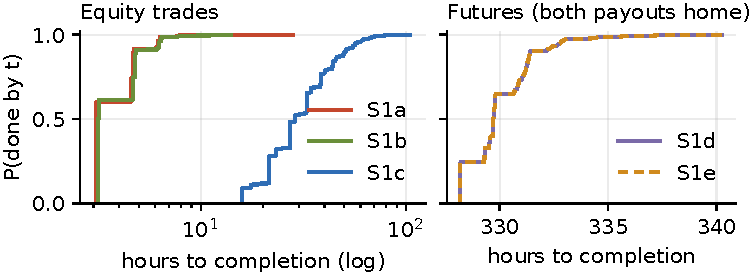
\includegraphics{figs/cdf.pdf}
\caption{Completion-time distributions under random loss (empirical CDF of the Monte Carlo runs in Table~A10). Left: the three equity trades, log scale. Right: the futures, both payouts home.}\label{fig:cdf}
\end{figure}

\section*{E3+. State histories and settlement moments}
Table~A13 is the opening balance sheet. For each scenario the next tables list every change in the
positions of its two parties, one row per account and asset that changed, so that the whole ledger history can be
read off without the trace files. ``Home'' is available at the home exchange, ``At host'' is available in the remote
trading account, ``Locked'' is order and instruction holds plus contract margin, and ``Transit'' is value debited at
one exchange and not yet credited at another. All other accounts are unchanged in every run.

{\tablefont\setlength{\tabcolsep}{3pt}
\begin{longtable}{@{}r>{\raggedright\arraybackslash}p{4.6cm}llrrrr@{}}
\caption{State history of S1a: Alice (Earth) buys 1,000 Ares from Bob (Mars) at \$100.}\label{tab:shS1a}\\\noalign{\vskip 1pt}\hline\noalign{\vskip 1pt}\textbf{h} & \textbf{Event} & \textbf{Account} & \textbf{Asset} & \textbf{Home} & \textbf{At host} & \textbf{Locked} & \textbf{Transit} \\\hline\noalign{\vskip 1pt}\endfirsthead
\multicolumn{8}{@{}l}{\textit{(continued)}}\\\noalign{\vskip 1pt}\hline\noalign{\vskip 1pt}\textbf{h} & \textbf{Event} & \textbf{Account} & \textbf{Asset} & \textbf{Home} & \textbf{At host} & \textbf{Locked} & \textbf{Transit} \\\hline\noalign{\vskip 1pt}\endhead
\hline\endfoot
0.0003 & Order admitted EQ-sell & Bob & Ares & 2,000 & 0 & 1,000 & 0 \\
0.0003 & Export EA-X1 (fund) & Alice & ND & \$50,000 & 0 & 0 & \$100,000 \\
1.6966 & Import EA-X1 (fund) & Alice & ND & \$50,000 & \$100,000 & 0 & 0 \\
2.5024 & Order admitted EQ-buy & Alice & ND & \$50,000 & 0 & \$100,000 & 0 \\
2.5024 & Fill 1,000 Ares @ \$100 & Alice & ND & \$50,000 & 0 & 0 & 0 \\
2.5024 & Fill 1,000 Ares @ \$100 & Alice & Ares & 0 & 1,000 & 0 & 0 \\
2.5024 & Fill 1,000 Ares @ \$100 & Bob & ND & \$150,000 & 0 & 0 & 0 \\
2.5024 & Fill 1,000 Ares @ \$100 & Bob & Ares & 2,000 & 0 & 0 & 0 \\
2.5024 & Export MA-X1 (auto fill) & Alice & Ares & 0 & 0 & 0 & 1,000 \\
3.0674 & Import MA-X1 (auto fill) & Alice & Ares & 1,000 & 0 & 0 & 0 \\
\end{longtable}}
{\tablefont\setlength{\tabcolsep}{3pt}
\begin{longtable}{@{}r>{\raggedright\arraybackslash}p{4.6cm}llrrrr@{}}
\caption{State history of S1b: Alice (Earth) buys 1,000 Belt from Cara (Ceres) at \$100.}\label{tab:shS1b}\\\noalign{\vskip 1pt}\hline\noalign{\vskip 1pt}\textbf{h} & \textbf{Event} & \textbf{Account} & \textbf{Asset} & \textbf{Home} & \textbf{At host} & \textbf{Locked} & \textbf{Transit} \\\hline\noalign{\vskip 1pt}\endfirsthead
\multicolumn{8}{@{}l}{\textit{(continued)}}\\\noalign{\vskip 1pt}\hline\noalign{\vskip 1pt}\textbf{h} & \textbf{Event} & \textbf{Account} & \textbf{Asset} & \textbf{Home} & \textbf{At host} & \textbf{Locked} & \textbf{Transit} \\\hline\noalign{\vskip 1pt}\endhead
\hline\endfoot
0.0003 & Order admitted EQB-sell & Cara & Belt & 0 & 0 & 1,000 & 0 \\
0.0003 & Export EA-X1 (fund) & Alice & ND & \$50,000 & 0 & 0 & \$100,000 \\
1.6697 & Import EA-X1 (fund) & Alice & ND & \$50,000 & \$100,000 & 0 & 0 \\
2.6085 & Order admitted EQB-buy & Alice & ND & \$50,000 & 0 & \$100,000 & 0 \\
2.6085 & Fill 1,000 Belt @ \$100 & Alice & ND & \$50,000 & 0 & 0 & 0 \\
2.6085 & Fill 1,000 Belt @ \$100 & Alice & Belt & 0 & 1,000 & 0 & 0 \\
2.6085 & Fill 1,000 Belt @ \$100 & Cara & ND & \$200,000 & 0 & 0 & 0 \\
2.6085 & Fill 1,000 Belt @ \$100 & Cara & Belt & 0 & 0 & 0 & 0 \\
2.6085 & Export CE-X1 (auto fill) & Alice & Belt & 0 & 0 & 0 & 1,000 \\
3.1644 & Import CE-X1 (auto fill) & Alice & Belt & 1,000 & 0 & 0 & 0 \\
\end{longtable}}
{\tablefont\setlength{\tabcolsep}{3pt}
\begin{longtable}{@{}r>{\raggedright\arraybackslash}p{4.6cm}llrrrr@{}}
\caption{State history of S1c: Eve (Uranus) buys 400 Terra from Fin (Earth) at \$100.}\label{tab:shS1c}\\\noalign{\vskip 1pt}\hline\noalign{\vskip 1pt}\textbf{h} & \textbf{Event} & \textbf{Account} & \textbf{Asset} & \textbf{Home} & \textbf{At host} & \textbf{Locked} & \textbf{Transit} \\\hline\noalign{\vskip 1pt}\endfirsthead
\multicolumn{8}{@{}l}{\textit{(continued)}}\\\noalign{\vskip 1pt}\hline\noalign{\vskip 1pt}\textbf{h} & \textbf{Event} & \textbf{Account} & \textbf{Asset} & \textbf{Home} & \textbf{At host} & \textbf{Locked} & \textbf{Transit} \\\hline\noalign{\vskip 1pt}\endhead
\hline\endfoot
0.0003 & Order admitted EQT-sell & Fin & Terra & 600 & 0 & 400 & 0 \\
0.0003 & Export UR-X1 (fund) & Eve & ND & \$10,000 & 0 & 0 & \$40,000 \\
7.9134 & Import UR-X1 (fund) & Eve & ND & \$10,000 & \$40,000 & 0 & 0 \\
13.1878 & Order admitted EQT-buy & Eve & ND & \$10,000 & 0 & \$40,000 & 0 \\
13.1878 & Fill 400 Terra @ \$100 & Eve & ND & \$10,000 & 0 & 0 & 0 \\
13.1878 & Fill 400 Terra @ \$100 & Eve & Terra & 0 & 400 & 0 & 0 \\
13.1878 & Fill 400 Terra @ \$100 & Fin & ND & \$90,000 & 0 & 0 & 0 \\
13.1878 & Fill 400 Terra @ \$100 & Fin & Terra & 600 & 0 & 0 & 0 \\
13.1878 & Export EA-X1 (auto fill) & Eve & Terra & 0 & 0 & 0 & 400 \\
15.8244 & Import EA-X1 (auto fill) & Eve & Terra & 400 & 0 & 0 & 0 \\
\end{longtable}}
{\tablefont\setlength{\tabcolsep}{3pt}
\begin{longtable}{@{}r>{\raggedright\arraybackslash}p{4.6cm}llrrrr@{}}
\caption{State history of S1d: capped futures, rising path, $Q = 2{,}000$ (Alice long, Cara short).}\label{tab:shS1d}\\\noalign{\vskip 1pt}\hline\noalign{\vskip 1pt}\textbf{h} & \textbf{Event} & \textbf{Account} & \textbf{Asset} & \textbf{Home} & \textbf{At host} & \textbf{Locked} & \textbf{Transit} \\\hline\noalign{\vskip 1pt}\endfirsthead
\multicolumn{8}{@{}l}{\textit{(continued)}}\\\noalign{\vskip 1pt}\hline\noalign{\vskip 1pt}\textbf{h} & \textbf{Event} & \textbf{Account} & \textbf{Asset} & \textbf{Home} & \textbf{At host} & \textbf{Locked} & \textbf{Transit} \\\hline\noalign{\vskip 1pt}\endhead
\hline\endfoot
0.0003 & Export EA-X1 (fund) & Alice & ND & \$70,000 & 0 & 0 & \$80,000 \\
0.0003 & Export CE-X1 (fund) & Cara & ND & \$20,000 & 0 & 0 & \$80,000 \\
1.4868 & Import CE-X1 (fund) & Cara & ND & \$20,000 & \$80,000 & 0 & 0 \\
1.6966 & Import EA-X1 (fund) & Alice & ND & \$70,000 & \$80,000 & 0 & 0 \\
2.1410 & Margin held F1 & Cara & ND & \$20,000 & 0 & \$80,000 & 0 \\
2.5024 & Margin held F1 & Alice & ND & \$70,000 & 0 & \$80,000 & 0 \\
326.5024 & Contract fixed F1 & Alice & ND & \$70,000 & \$130,000 & 0 & 0 \\
326.5024 & Contract fixed F1 & Cara & ND & \$20,000 & \$30,000 & 0 & 0 \\
326.5024 & Export MA-X1 (payout) & Alice & ND & \$70,000 & 0 & 0 & \$130,000 \\
326.5024 & Export MA-X2 (payout) & Cara & ND & \$20,000 & 0 & 0 & \$30,000 \\
328.0321 & Import MA-X2 (payout) & Cara & ND & \$50,000 & 0 & 0 & 0 \\
328.1736 & Import MA-X1 (payout) & Alice & ND & \$200,000 & 0 & 0 & 0 \\
\end{longtable}}
{\tablefont\setlength{\tabcolsep}{3pt}
\begin{longtable}{@{}r>{\raggedright\arraybackslash}p{4.6cm}llrrrr@{}}
\caption{State history of S1e: capped futures, falling path, $Q = 2{,}000$.}\label{tab:shS1e}\\\noalign{\vskip 1pt}\hline\noalign{\vskip 1pt}\textbf{h} & \textbf{Event} & \textbf{Account} & \textbf{Asset} & \textbf{Home} & \textbf{At host} & \textbf{Locked} & \textbf{Transit} \\\hline\noalign{\vskip 1pt}\endfirsthead
\multicolumn{8}{@{}l}{\textit{(continued)}}\\\noalign{\vskip 1pt}\hline\noalign{\vskip 1pt}\textbf{h} & \textbf{Event} & \textbf{Account} & \textbf{Asset} & \textbf{Home} & \textbf{At host} & \textbf{Locked} & \textbf{Transit} \\\hline\noalign{\vskip 1pt}\endhead
\hline\endfoot
0.0003 & Export EA-X1 (fund) & Alice & ND & \$70,000 & 0 & 0 & \$80,000 \\
0.0003 & Export CE-X1 (fund) & Cara & ND & \$20,000 & 0 & 0 & \$80,000 \\
1.4868 & Import CE-X1 (fund) & Cara & ND & \$20,000 & \$80,000 & 0 & 0 \\
1.6966 & Import EA-X1 (fund) & Alice & ND & \$70,000 & \$80,000 & 0 & 0 \\
2.1410 & Margin held F1 & Cara & ND & \$20,000 & 0 & \$80,000 & 0 \\
2.5024 & Margin held F1 & Alice & ND & \$70,000 & 0 & \$80,000 & 0 \\
326.5024 & Contract fixed F1 & Alice & ND & \$70,000 & \$30,000 & 0 & 0 \\
326.5024 & Contract fixed F1 & Cara & ND & \$20,000 & \$130,000 & 0 & 0 \\
326.5024 & Export MA-X1 (payout) & Alice & ND & \$70,000 & 0 & 0 & \$30,000 \\
326.5024 & Export MA-X2 (payout) & Cara & ND & \$20,000 & 0 & 0 & \$130,000 \\
328.0321 & Import MA-X2 (payout) & Cara & ND & \$150,000 & 0 & 0 & 0 \\
328.1736 & Import MA-X1 (payout) & Alice & ND & \$100,000 & 0 & 0 & 0 \\
\end{longtable}}
{\tablefont\setlength{\tabcolsep}{3pt}
\begin{longtable}{@{}r>{\raggedright\arraybackslash}p{4.6cm}llrrrr@{}}
\caption{State history of S1f: capped futures, boundary case $Q = 2{,}500$.}\label{tab:shS1f}\\\noalign{\vskip 1pt}\hline\noalign{\vskip 1pt}\textbf{h} & \textbf{Event} & \textbf{Account} & \textbf{Asset} & \textbf{Home} & \textbf{At host} & \textbf{Locked} & \textbf{Transit} \\\hline\noalign{\vskip 1pt}\endfirsthead
\multicolumn{8}{@{}l}{\textit{(continued)}}\\\noalign{\vskip 1pt}\hline\noalign{\vskip 1pt}\textbf{h} & \textbf{Event} & \textbf{Account} & \textbf{Asset} & \textbf{Home} & \textbf{At host} & \textbf{Locked} & \textbf{Transit} \\\hline\noalign{\vskip 1pt}\endhead
\hline\endfoot
0.0003 & Export EA-X1 (fund) & Alice & ND & \$50,000 & 0 & 0 & \$100,000 \\
0.0003 & Export CE-X1 (fund) & Cara & ND & 0 & 0 & 0 & \$100,000 \\
1.4868 & Import CE-X1 (fund) & Cara & ND & 0 & \$100,000 & 0 & 0 \\
1.6966 & Import EA-X1 (fund) & Alice & ND & \$50,000 & \$100,000 & 0 & 0 \\
2.1410 & Margin held F1 & Cara & ND & 0 & 0 & \$100,000 & 0 \\
2.5024 & Margin held F1 & Alice & ND & \$50,000 & 0 & \$100,000 & 0 \\
326.5024 & Contract fixed F1 & Alice & ND & \$50,000 & \$162,500 & 0 & 0 \\
326.5024 & Contract fixed F1 & Cara & ND & 0 & \$37,500 & 0 & 0 \\
326.5024 & Export MA-X1 (payout) & Alice & ND & \$50,000 & 0 & 0 & \$162,500 \\
326.5024 & Export MA-X2 (payout) & Cara & ND & 0 & 0 & 0 & \$37,500 \\
328.0321 & Import MA-X2 (payout) & Cara & ND & \$37,500 & 0 & 0 & 0 \\
328.1736 & Import MA-X1 (payout) & Alice & ND & \$212,500 & 0 & 0 & 0 \\
\end{longtable}}
{\tablefont\setlength{\tabcolsep}{3pt}
\begin{longtable}{@{}r>{\raggedright\arraybackslash}p{4.6cm}llrrrr@{}}
\caption{State history of S1g: capped futures, $Q = 2{,}501$ (Cara cannot fund; Alice is refunded).}\label{tab:shS1g}\\\noalign{\vskip 1pt}\hline\noalign{\vskip 1pt}\textbf{h} & \textbf{Event} & \textbf{Account} & \textbf{Asset} & \textbf{Home} & \textbf{At host} & \textbf{Locked} & \textbf{Transit} \\\hline\noalign{\vskip 1pt}\endfirsthead
\multicolumn{8}{@{}l}{\textit{(continued)}}\\\noalign{\vskip 1pt}\hline\noalign{\vskip 1pt}\textbf{h} & \textbf{Event} & \textbf{Account} & \textbf{Asset} & \textbf{Home} & \textbf{At host} & \textbf{Locked} & \textbf{Transit} \\\hline\noalign{\vskip 1pt}\endhead
\hline\endfoot
0.0003 & Export EA-X1 (fund) & Alice & ND & \$49,960 & 0 & 0 & \$100,040 \\
1.6966 & Import EA-X1 (fund) & Alice & ND & \$49,960 & \$100,040 & 0 & 0 \\
2.5024 & Margin held F1 & Alice & ND & \$49,960 & 0 & \$100,040 & 0 \\
168.0000 & Margin released F1 & Alice & ND & \$49,960 & \$100,040 & 0 & 0 \\
169.2336 & Export MA-X1 (withdraw) & Alice & ND & \$49,960 & 0 & 0 & \$100,040 \\
169.7939 & Import MA-X1 (withdraw) & Alice & ND & \$150,000 & 0 & 0 & 0 \\
\end{longtable}}
{\tablefont\setlength{\tabcolsep}{3pt}
\begin{longtable}{@{}r>{\raggedright\arraybackslash}p{4.6cm}llrrrr@{}}
\caption{State history of S1i: repeat trading on a \$10,000 Mars account.}\label{tab:shS1i}\\\noalign{\vskip 1pt}\hline\noalign{\vskip 1pt}\textbf{h} & \textbf{Event} & \textbf{Account} & \textbf{Asset} & \textbf{Home} & \textbf{At host} & \textbf{Locked} & \textbf{Transit} \\\hline\noalign{\vskip 1pt}\endfirsthead
\multicolumn{8}{@{}l}{\textit{(continued)}}\\\noalign{\vskip 1pt}\hline\noalign{\vskip 1pt}\textbf{h} & \textbf{Event} & \textbf{Account} & \textbf{Asset} & \textbf{Home} & \textbf{At host} & \textbf{Locked} & \textbf{Transit} \\\hline\noalign{\vskip 1pt}\endhead
\hline\endfoot
0.0003 & Export EA-X1 (fund) & Alice & ND & \$140,000 & 0 & 0 & \$10,000 \\
0.0003 & Order admitted RT-s1 & Bob & Ares & 2,990 & 0 & 10 & 0 \\
0.0003 & Order admitted RT-s2 & Bob & Ares & 2,985 & 0 & 15 & 0 \\
1.6966 & Import EA-X1 (fund) & Alice & ND & \$140,000 & \$10,000 & 0 & 0 \\
2.5024 & Order admitted RT-o1 & Alice & ND & \$140,000 & \$6,000 & \$4,000 & 0 \\
2.5024 & Fill 10 Ares @ \$97 & Alice & ND & \$140,000 & \$6,030 & \$3,000 & 0 \\
2.5024 & Fill 10 Ares @ \$97 & Alice & Ares & 0 & 10 & 0 & 0 \\
2.5024 & Fill 10 Ares @ \$97 & Bob & ND & \$50,970 & 0 & 0 & 0 \\
2.5024 & Fill 10 Ares @ \$97 & Bob & Ares & 2,985 & 0 & 5 & 0 \\
2.5024 & Fill 5 Ares @ \$100 & Alice & ND & \$140,000 & \$6,030 & \$2,500 & 0 \\
2.5024 & Fill 5 Ares @ \$100 & Alice & Ares & 0 & 15 & 0 & 0 \\
2.5024 & Fill 5 Ares @ \$100 & Bob & ND & \$51,470 & 0 & 0 & 0 \\
2.5024 & Fill 5 Ares @ \$100 & Bob & Ares & 2,985 & 0 & 0 & 0 \\
2.5024 & Order admitted RT-o2 & Alice & ND & \$140,000 & \$2,030 & \$6,500 & 0 \\
8.5021 & Cancelled RT-o2 & Alice & ND & \$140,000 & \$6,030 & \$2,500 & 0 \\
14.5019 & Order admitted RT-o3 & Alice & Ares & 0 & 5 & 10 & 0 \\
15.2627 & Order admitted RT-b1 & Bob & ND & \$50,460 & 0 & \$1,010 & 0 \\
15.2627 & Fill 10 Ares @ \$101 & Alice & ND & \$140,000 & \$7,040 & \$2,500 & 0 \\
15.2627 & Fill 10 Ares @ \$101 & Alice & Ares & 0 & 5 & 0 & 0 \\
15.2627 & Fill 10 Ares @ \$101 & Bob & ND & \$50,460 & 0 & 0 & 0 \\
15.2627 & Fill 10 Ares @ \$101 & Bob & Ares & 2,995 & 0 & 0 & 0 \\
26.3627 & Order admitted RT-s3 & Bob & Ares & 2,990 & 0 & 5 & 0 \\
26.3627 & Fill 5 Ares @ \$100 & Alice & ND & \$140,000 & \$7,040 & \$2,000 & 0 \\
26.3627 & Fill 5 Ares @ \$100 & Alice & Ares & 0 & 10 & 0 & 0 \\
26.3627 & Fill 5 Ares @ \$100 & Bob & ND & \$50,960 & 0 & 0 & 0 \\
26.3627 & Fill 5 Ares @ \$100 & Bob & Ares & 2,990 & 0 & 0 & 0 \\
26.5015 & Cancelled RT-o1 & Alice & ND & \$140,000 & \$9,040 & 0 & 0 \\
50.5006 & Export MA-X1 (withdraw) & Alice & ND & \$140,000 & 0 & 0 & \$9,040 \\
50.5006 & Export MA-X2 (withdraw) & Alice & Ares & 0 & 0 & 0 & 10 \\
51.0642 & Import MA-X1 (withdraw) & Alice & ND & \$149,040 & 0 & 0 & 0 \\
51.0642 & Import MA-X2 (withdraw) & Alice & Ares & 10 & 0 & 0 & 0 \\
\end{longtable}}

\paragraph{Settlement moments.} Table~\ref{tab:e3moments} lists every obligation in every scenario. An obligation is
\emph{discharged} when the duty it records is met (a fill, a fixing, or a transfer credited at its destination); a
claim is \emph{backed} once the value has been debited into a transfer, so nobody can spend it twice; and it is
\emph{spendable} when the owner can use it, either at the host or at home.

{\tablefont\setlength{\tabcolsep}{3pt}
\begin{longtable}{@{}l>{\raggedright\arraybackslash}p{5.2cm}rrll@{}}
\caption{Settlement moments of every obligation in every S1 scenario (hours, no loss).}\label{tab:e3moments}\\\noalign{\vskip 1pt}\hline\noalign{\vskip 1pt}\textbf{Run} & \textbf{Obligation} & \textbf{Created h} & \textbf{Discharged h} & \textbf{Backed} & \textbf{Spendable} \\\hline\noalign{\vskip 1pt}\endfirsthead
\multicolumn{6}{@{}l}{\textit{(continued)}}\\\noalign{\vskip 1pt}\hline\noalign{\vskip 1pt}\textbf{Run} & \textbf{Obligation} & \textbf{Created h} & \textbf{Discharged h} & \textbf{Backed} & \textbf{Spendable} \\\hline\noalign{\vskip 1pt}\endhead
\hline\endfoot
S1a & Fund \$100,000 for Alice, Ea→Ma & 0.000 & 1.697 & 0.000 & 1.697 at host \\
S1a & Fill 1,000 Ares @ \$100: Alice from Bob & 2.502 & 2.502 & local & 2.502 at host \\
S1a & Auto Fill 1,000 Ares for Alice, Ma→Ea & 2.502 & 3.067 & 2.502 & 3.067 at home \\
S1b & Fund \$100,000 for Alice, Ea→Ce & 0.000 & 1.670 & 0.000 & 1.670 at host \\
S1b & Fill 1,000 Belt @ \$100: Alice from Cara & 2.608 & 2.608 & local & 2.608 at host \\
S1b & Auto Fill 1,000 Belt for Alice, Ce→Ea & 2.608 & 3.164 & 2.608 & 3.164 at home \\
S1c & Fund \$40,000 for Eve, Ur→Ea & 0.000 & 7.913 & 0.000 & 7.913 at host \\
S1c & Fill 400 Terra @ \$100: Eve from Fin & 13.188 & 13.188 & local & 13.188 at host \\
S1c & Auto Fill 400 Terra for Eve, Ea→Ur & 13.188 & 15.824 & 13.188 & 15.824 at home \\
S1d & Fund \$80,000 for Alice, Ea→Ma & 0.000 & 1.697 & 0.000 & 1.697 at host \\
S1d & Fund \$80,000 for Cara, Ce→Ma & 0.000 & 1.487 & 0.000 & 1.487 at host \\
S1d & Contract F1 (escrow \$160,000) & 2.502 & at fixing & escrow from 2.502 & — \\
S1d & Fixing of F1 at 125 & 326.502 & 326.502 & 326.502 (payouts) & — \\
S1d & Payout \$130,000 for Alice, Ma→Ea & 326.502 & 328.174 & 326.502 & 328.174 at home \\
S1d & Payout \$30,000 for Cara, Ma→Ce & 326.502 & 328.032 & 326.502 & 328.032 at home \\
S1e & Fund \$80,000 for Alice, Ea→Ma & 0.000 & 1.697 & 0.000 & 1.697 at host \\
S1e & Fund \$80,000 for Cara, Ce→Ma & 0.000 & 1.487 & 0.000 & 1.487 at host \\
S1e & Contract F1 (escrow \$160,000) & 2.502 & at fixing & escrow from 2.502 & — \\
S1e & Fixing of F1 at 75 & 326.502 & 326.502 & 326.502 (payouts) & — \\
S1e & Payout \$30,000 for Alice, Ma→Ea & 326.502 & 328.174 & 326.502 & 328.174 at home \\
S1e & Payout \$130,000 for Cara, Ma→Ce & 326.502 & 328.032 & 326.502 & 328.032 at home \\
S1f & Fund \$100,000 for Alice, Ea→Ma & 0.000 & 1.697 & 0.000 & 1.697 at host \\
S1f & Fund \$100,000 for Cara, Ce→Ma & 0.000 & 1.487 & 0.000 & 1.487 at host \\
S1f & Contract F1 (escrow \$200,000) & 2.502 & at fixing & escrow from 2.502 & — \\
S1f & Fixing of F1 at 125 & 326.502 & 326.502 & 326.502 (payouts) & — \\
S1f & Payout \$162,500 for Alice, Ma→Ea & 326.502 & 328.174 & 326.502 & 328.174 at home \\
S1f & Payout \$37,500 for Cara, Ma→Ce & 326.502 & 328.032 & 326.502 & 328.032 at home \\
S1g & Fund \$100,040 for Alice, Ea→Ma & 0.000 & 1.697 & 0.000 & 1.697 at host \\
S1g & Withdraw \$100,040 for Alice, Ma→Ea & 169.234 & 169.794 & 169.234 & 169.794 at home \\
S1i & Fund \$10,000 for Alice, Ea→Ma & 0.000 & 1.697 & 0.000 & 1.697 at host \\
S1i & Fill 10 Ares @ \$97: Alice from Bob & 2.502 & 2.502 & local & 2.502 at host \\
S1i & Fill 5 Ares @ \$100: Alice from Bob & 2.502 & 2.502 & local & 2.502 at host \\
S1i & Fill 10 Ares @ \$101: Bob from Alice & 15.263 & 15.263 & local & 15.263 at host \\
S1i & Fill 5 Ares @ \$100: Alice from Bob & 26.363 & 26.363 & local & 26.363 at host \\
S1i & Withdraw \$9,040 for Alice, Ma→Ea & 50.501 & 51.064 & 50.501 & 51.064 at home \\
S1i & Withdraw 10 Ares for Alice, Ma→Ea & 50.501 & 51.064 & 50.501 & 51.064 at home \\
\end{longtable}}

\section*{S2+. Incident search and complete trace}
\begin{figure}[!htb]\centering
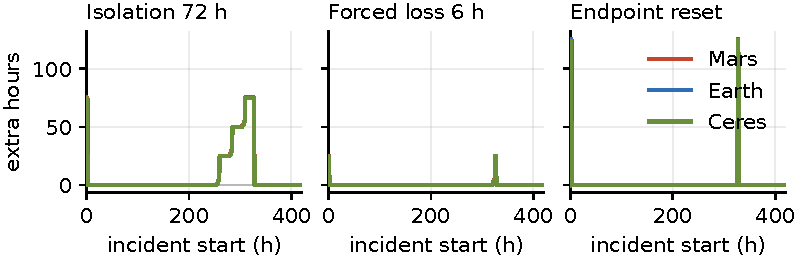
\includegraphics{figs/s2_search.pdf}
\caption{Damage (extra hours until both payouts are home, capped at 200) against incident start time on the rising path. Coloured lines are the three exchanges in the scenario; grey lines are the other nodes.}\label{fig:s2}
\end{figure}

We chose the endpoint reset of the Mars exchange at hour 0.75, which is the worst incident on both
price paths. It does more damage than the obvious choice, isolating the host at payout time (about 75 hours), even
though no party can observe it. At hour 0.75, Mars has just answered Alice's and Cara's handshakes. The reset
erases its session state, but its SYN-ACK replies are already in flight. Earth and Ceres therefore believe that the
sessions are open and send their funding transfers into sessions that Mars no longer knows. As the brief requires,
Mars ignores them. The senders learn nothing until four endpoint attempts of $R_e \approx 25$ hours have expired. They
then wait for the 24-hour application backoff and resubmit. The courier log of the rising path shows this sequence.
Earth and Ceres open their sessions with Mars at hour 0.0003. Ceres declares its delivery unknown at
hour 100.97 and Earth at hour 101.64. Each schedules an application
resubmission 24 hours later, and they resubmit in new sessions at hours 124.97 and
125.64.

\paragraph{Complete trace of the incident.} Table~\ref{tab:s2trace} lists every event of the selected incident up to
the opening; the files \texttt{traces/S2\_reset\_Mars\_\{launches,transport,ledger\}.csv} hold the whole run, including
the 300-hour contract and the payouts, which then follow S1d shifted by the delay. The table shows the four steps of
the 125-hour penalty: the handshakes complete before the reset, so Earth and Ceres send their transfers into sessions
Mars has forgotten; Mars ignores every copy; each sender's four endpoint attempts expire (delivery unknown); and
after the 24-hour application backoff each resubmits on a new session, which succeeds within about two hours.

{\tablefont\setlength{\tabcolsep}{3pt}
\begin{longtable}{@{}rll>{\raggedright\arraybackslash}p{8.2cm}@{}}
\caption{Event-by-event trace of the S2 incident (rising path, no loss) from hour 0 to the opening at 128.126: every backbone launch except the 66 hop receipts, every direct copy, every courier event and every ledger event. Ea = Earth, Ma = Mars, Ce = Ceres, A = Relay A.}\label{tab:s2trace}\\\noalign{\vskip 1pt}\hline\noalign{\vskip 1pt}\textbf{h} & \textbf{At} & \textbf{Event} & \textbf{Detail} \\\hline\noalign{\vskip 1pt}\endfirsthead
\multicolumn{4}{@{}l}{\textit{(continued)}}\\\noalign{\vskip 1pt}\hline\noalign{\vskip 1pt}\textbf{h} & \textbf{At} & \textbf{Event} & \textbf{Detail} \\\hline\noalign{\vskip 1pt}\endhead
\hline\endfoot
0.000 & Earth & session open & session s26 to Mars via Earth, Relay A, Mars \\
0.000 & Ceres & session open & session s27 to Mars via Ceres, Relay A, Mars \\
0.000 & Alice & local instruction & FUND \$80,000 to Mars \\
0.000 & Earth & export & EA-X1: \$80,000 of Alice debited, in transit to Mars \\
0.000 & Cara & local instruction & FUND \$80,000 to Mars \\
0.000 & Ceres & export & CE-X1: \$80,000 of Cara debited, in transit to Mars \\
0.001 & Ce→A & launch & SYN s27, arrives 0.243 \\
0.001 & Ea→A & launch & SYN s26, arrives 0.313 \\
0.244 & A→Ma & launch & SYN s27, arrives 0.495 \\
0.314 & A→Ma & launch & SYN s26, arrives 0.565 \\
0.496 & Ma→A & launch & SYNACK s27, arrives 0.748 \\
0.566 & Ma→A & launch & SYNACK s26, arrives 0.818 \\
0.748 & A→Ce & launch & SYNACK s27, arrives 0.991 \\
0.750 & Mars & endpoint reset & all session state lost; ledger and durable outbox kept \\
0.818 & A→Ea & launch & SYNACK s26, arrives 1.131 \\
0.992 & Ce→A & launch & ACK s27, arrives 1.234 \\
0.992 & Ce→A & launch & DATA s27 (carries DATA), arrives 1.235 \\
1.131 & Ea→A & launch & ACK s26, arrives 1.444 \\
1.132 & Ea→A & launch & DATA s26 (carries DATA), arrives 1.444 \\
1.235 & A→Ma & launch & ACK s27, arrives 1.487 \\
1.235 & A→Ma & launch & DATA s27 (carries DATA), arrives 1.487 \\
1.445 & A→Ma & launch & ACK s26, arrives 1.696 \\
1.445 & A→Ma & launch & DATA s26 (carries DATA), arrives 1.697 \\
1.487 & Mars & ignored & ACK on s27 from Ceres: Mars lost this session in the reset \\
1.487 & Mars & ignored & DATA on s27 from Ceres: Mars lost this session in the reset \\
1.696 & Mars & ignored & ACK on s26 from Earth: Mars lost this session in the reset \\
1.697 & Mars & ignored & DATA on s26 from Earth: Mars lost this session in the reset \\
25.982 & Ce→A & launch & DATA s27 (carries DATA), arrives 26.225 \\
26.225 & A→Ma & launch & DATA s27 (carries DATA), arrives 26.478 \\
26.261 & Ea→A & launch & DATA s26 (carries DATA), arrives 26.572 \\
26.478 & Mars & ignored & DATA on s27 from Ceres: Mars lost this session in the reset \\
26.573 & A→Ma & launch & DATA s26 (carries DATA), arrives 26.826 \\
26.826 & Mars & ignored & DATA on s26 from Earth: Mars lost this session in the reset \\
50.974 & Ce→A & launch & DATA s27 (carries DATA), arrives 51.217 \\
51.218 & A→Ma & launch & DATA s27 (carries DATA), arrives 51.472 \\
51.390 & Ea→A & launch & DATA s26 (carries DATA), arrives 51.699 \\
51.472 & Mars & ignored & DATA on s27 from Ceres: Mars lost this session in the reset \\
51.700 & A→Ma & launch & DATA s26 (carries DATA), arrives 51.954 \\
51.954 & Mars & ignored & DATA on s26 from Earth: Mars lost this session in the reset \\
75.969 & Ce→A & launch & DATA s27 (carries DATA), arrives 76.212 \\
76.213 & A→Ma & launch & DATA s27 (carries DATA), arrives 76.467 \\
76.467 & Mars & ignored & DATA on s27 from Ceres: Mars lost this session in the reset \\
76.518 & Ea→A & launch & DATA s26 (carries DATA), arrives 76.825 \\
76.826 & A→Ma & launch & DATA s26 (carries DATA), arrives 77.080 \\
77.080 & Mars & ignored & DATA on s26 from Earth: Mars lost this session in the reset \\
100.966 & Ceres & delivery unknown & s27 to Mars: four endpoint attempts unacknowledged \\
100.966 & Ceres & app resubmit scheduled & resubmission of the transfer scheduled for 124.966 \\
101.643 & Earth & delivery unknown & s26 to Mars: four endpoint attempts unacknowledged \\
101.643 & Earth & app resubmit scheduled & resubmission of the transfer scheduled for 125.643 \\
124.966 & Ceres & app resubmit & transfer resubmitted to Mars on a new session \\
124.966 & Ceres & session open & session s28 to Mars via Ceres, Relay A, Mars \\
124.966 & Ce→A & launch & SYN s28, arrives 125.209 \\
125.210 & A→Ma & launch & SYN s28, arrives 125.467 \\
125.467 & Ma→A & launch & SYNACK s28, arrives 125.724 \\
125.643 & Earth & app resubmit & transfer resubmitted to Mars on a new session \\
125.643 & Earth & session open & session s29 to Mars via Earth, Relay A, Mars \\
125.643 & Ea→A & launch & SYN s29, arrives 125.948 \\
125.724 & A→Ce & launch & SYNACK s28, arrives 125.967 \\
125.948 & A→Ma & launch & SYN s29, arrives 126.205 \\
125.968 & Ce→A & launch & ACK s28, arrives 126.211 \\
125.968 & Ce→A & launch & DATA s28 (carries DATA), arrives 126.211 \\
126.205 & Ma→A & launch & SYNACK s29, arrives 126.462 \\
126.212 & A→Ma & launch & ACK s28, arrives 126.468 \\
126.212 & A→Ma & launch & DATA s28 (carries DATA), arrives 126.469 \\
126.463 & A→Ea & launch & SYNACK s29, arrives 126.767 \\
126.469 & Mars & import & CE-X1: \$80,000 credited to Cara \\
126.469 & Mars & received queued & RECEIVED for CE-X1 queued to Ceres \\
126.469 & Ma→A & launch & DACK s28, arrives 126.726 \\
126.470 & Ma→A & launch & DATA s28 (carries DATA), arrives 126.726 \\
126.726 & A→Ce & launch & DACK s28, arrives 126.970 \\
126.727 & A→Ce & launch & DATA s28 (carries DATA), arrives 126.970 \\
126.767 & Ea→A & launch & ACK s29, arrives 127.071 \\
126.767 & Ea→A & launch & DATA s29 (carries DATA), arrives 127.071 \\
126.970 & Ceres & receipt known & CE-X1 resolved \\
126.970 & Ce→A & launch & DACK s28, arrives 127.214 \\
126.971 & Ce→Ma & launch & direct CINSTR copy 1 from Cara, arrives 127.127 \\
126.987 & Ce→Ma & launch & direct CINSTR copy 2 from Cara, arrives 127.143 \\
127.072 & A→Ma & launch & ACK s29, arrives 127.328 \\
127.072 & A→Ma & launch & DATA s29 (carries DATA), arrives 127.329 \\
127.127 & Mars & margin held & Cara: \$80,000 margin held \\
127.127 & Mars & status queued & STATUS record to Ceres \\
127.127 & Ma→A & launch & DATA s28 (carries DATA), arrives 127.384 \\
127.143 & Mars & duplicate cinstr & later copy from Cara ignored \\
127.214 & A→Ma & launch & DACK s28, arrives 127.471 \\
127.329 & Mars & import & EA-X1: \$80,000 credited to Alice \\
127.329 & Mars & received queued & RECEIVED for EA-X1 queued to Earth \\
127.329 & Ma→A & launch & DACK s29, arrives 127.586 \\
127.329 & Ma→A & launch & DATA s29 (carries DATA), arrives 127.586 \\
127.384 & A→Ce & launch & DATA s28 (carries DATA), arrives 127.627 \\
127.586 & A→Ea & launch & DACK s29, arrives 127.890 \\
127.587 & A→Ea & launch & DATA s29 (carries DATA), arrives 127.891 \\
127.627 & Ceres & status received & Cara told HELD \\
127.628 & Ce→A & launch & DACK s28, arrives 127.871 \\
127.872 & A→Ma & launch & DACK s28, arrives 128.128 \\
127.891 & Earth & receipt known & EA-X1 resolved \\
127.891 & Ea→A & launch & DACK s29, arrives 128.195 \\
127.891 & Ea→Ma & launch & direct CINSTR copy 1 from Alice, arrives 128.126 \\
127.908 & Ea→Ma & launch & direct CINSTR copy 2 from Alice, arrives 128.143 \\
127.925 & Ea→Ma & launch & direct CINSTR copy 3 from Alice, arrives 128.159 \\
128.126 & Mars & margin held & Alice: \$80,000 margin held \\
128.126 & Mars & contract open & F1 opens, escrow \$160,000 \\
128.126 & Mars & status queued & STATUS record to Earth \\
128.126 & Mars & status queued & STATUS record to Ceres \\
128.126 & Ma→A & launch & DATA s29 (carries DATA), arrives 128.383 \\
128.127 & Ma→A & launch & DATA s28 (carries DATA), arrives 128.383 \\
128.143 & Mars & duplicate cinstr & later copy from Alice ignored \\
128.159 & Mars & duplicate cinstr & later copy from Alice ignored \\
128.196 & A→Ma & launch & DACK s29, arrives 128.452 \\
128.384 & A→Ea & launch & DATA s29 (carries DATA), arrives 128.688 \\
128.384 & A→Ce & launch & DATA s28 (carries DATA), arrives 128.627 \\
128.627 & Ceres & status received & Cara told OPEN \\
128.628 & Ce→A & launch & DACK s28, arrives 128.871 \\
128.688 & Earth & status received & Alice told OPEN \\
128.688 & Ea→A & launch & DACK s29, arrives 128.992 \\
128.871 & A→Ma & launch & DACK s28, arrives 129.128 \\
128.992 & A→Ma & launch & DACK s29, arrives 129.249 \\
\end{longtable}}


\section*{S3+. Complete relocation traces}
\paragraph{S3 relocations.} The same \$100,000 Ares purchase with Alice's account moved to the best, median and worst
homes of Table~A19.

{\tablefont\setlength{\tabcolsep}{3pt}
\begin{longtable}{@{}>{\raggedright\arraybackslash}p{0.55in}>{\raggedright\arraybackslash}p{0.6in}>{\raggedright\arraybackslash}p{0.72in}>{\raggedright\arraybackslash}p{1.05in}>{\raggedright\arraybackslash}p{1.05in}>{\raggedright\arraybackslash}p{0.55in}>{\raggedright\arraybackslash}p{1.45in}@{}}
\caption{Complete trace of the S3 relocation, best home: Alice at Ceres buys 1,000 Ares from Bob (Mars). Every ledger event, direct message and status message is shown.}\label{tab:trS3Ceres}\\\noalign{\vskip 1pt}\hline\noalign{\vskip 1pt}\textbf{h} & \textbf{Actor} & \textbf{Knows} & \textbf{Does} & \textbf{Packet or transmission} & \textbf{Arrives} & \textbf{Financial state after} \\\hline\noalign{\vskip 1pt}\endfirsthead
\multicolumn{7}{@{}l}{\textit{(continued)}}\\\noalign{\vskip 1pt}\hline\noalign{\vskip 1pt}\textbf{h} & \textbf{Actor} & \textbf{Knows} & \textbf{Does} & \textbf{Packet or transmission} & \textbf{Arrives} & \textbf{Financial state after} \\\hline\noalign{\vskip 1pt}\endhead
\hline\endfoot
0.0003 & Bob & Own inventory at the market & Sell 1,000 Ares limit \$100 GTC & Local access at Mars, sent h 0.0000 & 0.0003 & \textbf{Alice} \$150k at Ceres; \textbf{Bob} \$50k at Mars, 3,000 Ares home \\
0.0003 & Mars exchange & Its own available balances & Admits Bob EQ-sell; holds 1,000 Ares & — & — & \textbf{Alice} \$150k at Ceres; \textbf{Bob} \$50k at Mars, 2,000 Ares home, 1,000 Ares held \\
0.0003 & Alice & Listing table: Ares trades at Mars & QUOTE for Ares & Local access at Ceres, sent h 0.0000 & 0.0003 & \textbf{Alice} \$150k at Ceres; \textbf{Bob} \$50k at Mars, 2,000 Ares home, 1,000 Ares held \\
0.0003 & Ceres exchange & No fresh Ares snapshot on its board & Quote request (MDREQ) for Ares to Mars & Backbone Ce→Ma, batched with queued records & 1.4868 & \textbf{Alice} \$150k at Ceres; \textbf{Bob} \$50k at Mars, 2,000 Ares home, 1,000 Ares held \\
0.0003 & Alice & Own Ceres balance & Funds own Mars account: \$100k & Local access at Ceres, sent h 0.0000 & 0.0003 & \textbf{Alice} \$150k at Ceres; \textbf{Bob} \$50k at Mars, 2,000 Ares home, 1,000 Ares held \\
0.0003 & Ceres exchange & Instruction or fill; its own ledger & Debits Alice \$100k; TRANSFER CE-X1 (funding) to Mars & New session (SYN h 0.0006); DATA Ce→A h 0.9918, A→Ma h 1.2351 & 1.4868 & \textbf{Alice} \$50k at Ceres, \$100k in transit; \textbf{Bob} \$50k at Mars, 2,000 Ares home, 1,000 Ares held \\
1.4868 & Mars exchange & Its own live book & Replies with Ares snapshot (MDS, version 1) & Backbone Ma→Ce, batched with queued records & 1.9826 & \textbf{Alice} \$50k at Ceres, \$100k in transit; \textbf{Bob} \$50k at Mars, 2,000 Ares home, 1,000 Ares held \\
1.4868 & Mars exchange & Authentic new transfer CE-X1 & Imports once; credits Alice \$100k (spendable now) & RECEIVED to Ceres (backbone) & 1.9826 & \textbf{Alice} \$50k at Ceres, \$100k free at host; \textbf{Bob} \$50k at Mars, 2,000 Ares home, 1,000 Ares held \\
1.9826 & Ceres exchange & MDS from Mars & Posts Ares snapshot to its board (0.50 h old); answers waiting QUOTEs & Local access (1 s) & 1.9829 & \textbf{Alice} \$50k at Ceres, \$100k free at host; \textbf{Bob} \$50k at Mars, 2,000 Ares home, 1,000 Ares held \\
1.9826 & Ceres exchange & Mars imported CE-X1 & Marks transfer delivered; no balance change & — & — & \textbf{Alice} \$50k at Ceres, \$100k free at host; \textbf{Bob} \$50k at Mars, 2,000 Ares home, 1,000 Ares held \\
1.9829 & Alice & Home board (local access) & Reads Ares quote: bid none, ask \$100 × 1,000, 0.50 h old & — & — & \textbf{Alice} \$50k at Ceres, \$100k free at host; \textbf{Bob} \$50k at Mars, 2,000 Ares home, 1,000 Ares held \\
1.9829 & Alice & Published geometry; own funding confirmed & Sends ORDER ×2 copies & Direct Ce→Ma, launches 1.9829, 1.9996; p(loss) 0.087 each, all lost 7.5e-03 & 2.1410 (first) & \textbf{Alice} \$50k at Ceres, \$100k free at host; \textbf{Bob} \$50k at Mars, 2,000 Ares home, 1,000 Ares held \\
2.1410 & Mars exchange & Its own available balances & Admits Alice EQ-buy; holds \$100k & — & — & \textbf{Alice} \$50k at Ceres, \$100k held; \textbf{Bob} \$50k at Mars, 2,000 Ares home, 1,000 Ares held \\
2.1410 & Mars exchange & Both holds in its own ledger & Fill 1,000 Ares @ \$100: Alice buys from Bob & — & local, atomic & \textbf{Alice} \$50k at Ceres, 1,000 Ares at market; \textbf{Bob} \$150k at Mars, 2,000 Ares home \\
2.1410 & Mars exchange & Instruction or fill; its own ledger & Debits Alice 1,000 Ares; TRANSFER MA-X1 (automatic home delivery) to Ceres & Session from h 0.0006; DATA Ma→A h 2.1412, A→Ce h 2.3935 & 2.6363 & \textbf{Alice} \$50k at Ceres, 1,000 Ares in transit; \textbf{Bob} \$150k at Mars, 2,000 Ares home \\
2.1576 & Mars exchange & Same order already decided (ACCEPTED) & Ignores the copy; returns the original result & — & — & \textbf{Alice} \$50k at Ceres, 1,000 Ares in transit; \textbf{Bob} \$150k at Mars, 2,000 Ares home \\
2.6363 & Ceres exchange & Authentic new transfer MA-X1 & Imports once; credits Alice 1,000 Ares (spendable now) & RECEIVED to Mars (backbone) & 3.1321 & \textbf{Alice} \$50k at Ceres, 1,000 Ares home; \textbf{Bob} \$150k at Mars, 2,000 Ares home \\
3.1321 & Mars exchange & Ceres imported MA-X1 & Marks transfer delivered; no balance change & — & — & \textbf{Alice} \$50k at Ceres, 1,000 Ares home; \textbf{Bob} \$150k at Mars, 2,000 Ares home \\
\end{longtable}}
{\tablefont\setlength{\tabcolsep}{3pt}
\begin{longtable}{@{}>{\raggedright\arraybackslash}p{0.55in}>{\raggedright\arraybackslash}p{0.6in}>{\raggedright\arraybackslash}p{0.72in}>{\raggedright\arraybackslash}p{1.05in}>{\raggedright\arraybackslash}p{1.05in}>{\raggedright\arraybackslash}p{0.55in}>{\raggedright\arraybackslash}p{1.45in}@{}}
\caption{Complete trace of the S3 relocation, median home: Alice at Mercury buys 1,000 Ares from Bob (Mars). Every ledger event, direct message and status message is shown.}\label{tab:trS3Mercury}\\\noalign{\vskip 1pt}\hline\noalign{\vskip 1pt}\textbf{h} & \textbf{Actor} & \textbf{Knows} & \textbf{Does} & \textbf{Packet or transmission} & \textbf{Arrives} & \textbf{Financial state after} \\\hline\noalign{\vskip 1pt}\endfirsthead
\multicolumn{7}{@{}l}{\textit{(continued)}}\\\noalign{\vskip 1pt}\hline\noalign{\vskip 1pt}\textbf{h} & \textbf{Actor} & \textbf{Knows} & \textbf{Does} & \textbf{Packet or transmission} & \textbf{Arrives} & \textbf{Financial state after} \\\hline\noalign{\vskip 1pt}\endhead
\hline\endfoot
0.0003 & Bob & Own inventory at the market & Sell 1,000 Ares limit \$100 GTC & Local access at Mars, sent h 0.0000 & 0.0003 & \textbf{Alice} \$150k at Mercury; \textbf{Bob} \$50k at Mars, 3,000 Ares home \\
0.0003 & Mars exchange & Its own available balances & Admits Bob EQ-sell; holds 1,000 Ares & — & — & \textbf{Alice} \$150k at Mercury; \textbf{Bob} \$50k at Mars, 2,000 Ares home, 1,000 Ares held \\
0.0003 & Alice & Listing table: Ares trades at Mars & QUOTE for Ares & Local access at Mercury, sent h 0.0000 & 0.0003 & \textbf{Alice} \$150k at Mercury; \textbf{Bob} \$50k at Mars, 2,000 Ares home, 1,000 Ares held \\
0.0003 & Mercury exchange & No fresh Ares snapshot on its board & Quote request (MDREQ) for Ares to Mars & Backbone Me→Ma, batched with queued records & 2.1195 & \textbf{Alice} \$150k at Mercury; \textbf{Bob} \$50k at Mars, 2,000 Ares home, 1,000 Ares held \\
0.0003 & Alice & Own Mercury balance & Funds own Mars account: \$100k & Local access at Mercury, sent h 0.0000 & 0.0003 & \textbf{Alice} \$150k at Mercury; \textbf{Bob} \$50k at Mars, 2,000 Ares home, 1,000 Ares held \\
0.0003 & Mercury exchange & Instruction or fill; its own ledger & Debits Alice \$100k; TRANSFER ME-X1 (funding) to Mars & New session (SYN h 0.0006); DATA Me→A h 1.4136, A→Ma h 1.8678 & 2.1195 & \textbf{Alice} \$50k at Mercury, \$100k in transit; \textbf{Bob} \$50k at Mars, 2,000 Ares home, 1,000 Ares held \\
2.1195 & Mars exchange & Its own live book & Replies with Ares snapshot (MDS, version 1) & Backbone Ma→Me, batched with queued records & 2.8262 & \textbf{Alice} \$50k at Mercury, \$100k in transit; \textbf{Bob} \$50k at Mars, 2,000 Ares home, 1,000 Ares held \\
2.1195 & Mars exchange & Authentic new transfer ME-X1 & Imports once; credits Alice \$100k (spendable now) & RECEIVED to Mercury (backbone) & 2.8262 & \textbf{Alice} \$50k at Mercury, \$100k free at host; \textbf{Bob} \$50k at Mars, 2,000 Ares home, 1,000 Ares held \\
2.8262 & Mercury exchange & MDS from Mars & Posts Ares snapshot to its board (0.71 h old); answers waiting QUOTEs & Local access (1 s) & 2.8264 & \textbf{Alice} \$50k at Mercury, \$100k free at host; \textbf{Bob} \$50k at Mars, 2,000 Ares home, 1,000 Ares held \\
2.8262 & Mercury exchange & Mars imported ME-X1 & Marks transfer delivered; no balance change & — & — & \textbf{Alice} \$50k at Mercury, \$100k free at host; \textbf{Bob} \$50k at Mars, 2,000 Ares home, 1,000 Ares held \\
2.8264 & Alice & Home board (local access) & Reads Ares quote: bid none, ask \$100 × 1,000, 0.71 h old & — & — & \textbf{Alice} \$50k at Mercury, \$100k free at host; \textbf{Bob} \$50k at Mars, 2,000 Ares home, 1,000 Ares held \\
2.8264 & Alice & Published geometry; own funding confirmed & Sends ORDER ×3 copies & Direct Me→Ma, launches 2.8264, 2.8431, 2.8598; p(loss) 0.147 each, all lost 3.2e-03 & 3.1035 (first) & \textbf{Alice} \$50k at Mercury, \$100k free at host; \textbf{Bob} \$50k at Mars, 2,000 Ares home, 1,000 Ares held \\
3.1035 & Mars exchange & Its own available balances & Admits Alice EQ-buy; holds \$100k & — & — & \textbf{Alice} \$50k at Mercury, \$100k held; \textbf{Bob} \$50k at Mars, 2,000 Ares home, 1,000 Ares held \\
3.1035 & Mars exchange & Both holds in its own ledger & Fill 1,000 Ares @ \$100: Alice buys from Bob & — & local, atomic & \textbf{Alice} \$50k at Mercury, 1,000 Ares at market; \textbf{Bob} \$150k at Mars, 2,000 Ares home \\
3.1035 & Mars exchange & Instruction or fill; its own ledger & Debits Alice 1,000 Ares; TRANSFER MA-X1 (automatic home delivery) to Mercury & Session from h 0.0006; DATA Ma→A h 3.1037, A→Me h 3.3561 & 3.8096 & \textbf{Alice} \$50k at Mercury, 1,000 Ares in transit; \textbf{Bob} \$150k at Mars, 2,000 Ares home \\
3.1201 & Mars exchange & Same order already decided (ACCEPTED) & Ignores the copy; returns the original result & — & — & \textbf{Alice} \$50k at Mercury, 1,000 Ares in transit; \textbf{Bob} \$150k at Mars, 2,000 Ares home \\
3.1368 & Mars exchange & Same order already decided (ACCEPTED) & Ignores the copy; returns the original result & — & — & \textbf{Alice} \$50k at Mercury, 1,000 Ares in transit; \textbf{Bob} \$150k at Mars, 2,000 Ares home \\
3.8096 & Mercury exchange & Authentic new transfer MA-X1 & Imports once; credits Alice 1,000 Ares (spendable now) & RECEIVED to Mars (backbone) & 4.5163 & \textbf{Alice} \$50k at Mercury, 1,000 Ares home; \textbf{Bob} \$150k at Mars, 2,000 Ares home \\
4.5163 & Mars exchange & Mercury imported MA-X1 & Marks transfer delivered; no balance change & — & — & \textbf{Alice} \$50k at Mercury, 1,000 Ares home; \textbf{Bob} \$150k at Mars, 2,000 Ares home \\
\end{longtable}}
{\tablefont\setlength{\tabcolsep}{3pt}
\begin{longtable}{@{}>{\raggedright\arraybackslash}p{0.55in}>{\raggedright\arraybackslash}p{0.6in}>{\raggedright\arraybackslash}p{0.72in}>{\raggedright\arraybackslash}p{1.05in}>{\raggedright\arraybackslash}p{1.05in}>{\raggedright\arraybackslash}p{0.55in}>{\raggedright\arraybackslash}p{1.45in}@{}}
\caption{Complete trace of the S3 relocation, worst home: Alice at Neptune buys 1,000 Ares from Bob (Mars). Every ledger event, direct message and status message is shown.}\label{tab:trS3Neptune}\\\noalign{\vskip 1pt}\hline\noalign{\vskip 1pt}\textbf{h} & \textbf{Actor} & \textbf{Knows} & \textbf{Does} & \textbf{Packet or transmission} & \textbf{Arrives} & \textbf{Financial state after} \\\hline\noalign{\vskip 1pt}\endfirsthead
\multicolumn{7}{@{}l}{\textit{(continued)}}\\\noalign{\vskip 1pt}\hline\noalign{\vskip 1pt}\textbf{h} & \textbf{Actor} & \textbf{Knows} & \textbf{Does} & \textbf{Packet or transmission} & \textbf{Arrives} & \textbf{Financial state after} \\\hline\noalign{\vskip 1pt}\endhead
\hline\endfoot
0.0003 & Bob & Own inventory at the market & Sell 1,000 Ares limit \$100 GTC & Local access at Mars, sent h 0.0000 & 0.0003 & \textbf{Alice} \$150k at Neptune; \textbf{Bob} \$50k at Mars, 3,000 Ares home \\
0.0003 & Mars exchange & Its own available balances & Admits Bob EQ-sell; holds 1,000 Ares & — & — & \textbf{Alice} \$150k at Neptune; \textbf{Bob} \$50k at Mars, 2,000 Ares home, 1,000 Ares held \\
0.0003 & Alice & Listing table: Ares trades at Mars & QUOTE for Ares & Local access at Neptune, sent h 0.0000 & 0.0003 & \textbf{Alice} \$150k at Neptune; \textbf{Bob} \$50k at Mars, 2,000 Ares home, 1,000 Ares held \\
0.0003 & Neptune exchange & No fresh Ares snapshot on its board & Quote request (MDREQ) for Ares to Mars & Backbone Ne→Ma, batched with queued records & 12.3441 & \textbf{Alice} \$150k at Neptune; \textbf{Bob} \$50k at Mars, 2,000 Ares home, 1,000 Ares held \\
0.0003 & Alice & Own Neptune balance & Funds own Mars account: \$100k & Local access at Neptune, sent h 0.0000 & 0.0003 & \textbf{Alice} \$150k at Neptune; \textbf{Bob} \$50k at Mars, 2,000 Ares home, 1,000 Ares held \\
0.0003 & Neptune exchange & Instruction or fill; its own ledger & Debits Alice \$100k; TRANSFER NE-X1 (funding) to Mars & New session (SYN h 0.0006); DATA Ne→A h 8.2296, A→Ma h 12.0919 & 12.3441 & \textbf{Alice} \$50k at Neptune, \$100k in transit; \textbf{Bob} \$50k at Mars, 2,000 Ares home, 1,000 Ares held \\
12.3441 & Mars exchange & Its own live book & Replies with Ares snapshot (MDS, version 1) & Backbone Ma→Ne, batched with queued records & 16.4594 & \textbf{Alice} \$50k at Neptune, \$100k in transit; \textbf{Bob} \$50k at Mars, 2,000 Ares home, 1,000 Ares held \\
12.3441 & Mars exchange & Authentic new transfer NE-X1 & Imports once; credits Alice \$100k (spendable now) & RECEIVED to Neptune (backbone) & 16.4594 & \textbf{Alice} \$50k at Neptune, \$100k free at host; \textbf{Bob} \$50k at Mars, 2,000 Ares home, 1,000 Ares held \\
16.4594 & Neptune exchange & MDS from Mars & Posts Ares snapshot to its board (4.12 h old); answers waiting QUOTEs & Local access (1 s) & 16.4597 & \textbf{Alice} \$50k at Neptune, \$100k free at host; \textbf{Bob} \$50k at Mars, 2,000 Ares home, 1,000 Ares held \\
16.4594 & Neptune exchange & Mars imported NE-X1 & Marks transfer delivered; no balance change & — & — & \textbf{Alice} \$50k at Neptune, \$100k free at host; \textbf{Bob} \$50k at Mars, 2,000 Ares home, 1,000 Ares held \\
16.4597 & Alice & Home board (local access) & Reads Ares quote: bid none, ask \$100 × 1,000, 4.12 h old & — & — & \textbf{Alice} \$50k at Neptune, \$100k free at host; \textbf{Bob} \$50k at Mars, 2,000 Ares home, 1,000 Ares held \\
16.4597 & Alice & Published geometry; own funding confirmed & Sends ORDER ×8 copies & Direct Ne→Ma, launches 16.4597, 16.4763, 16.4930, 16.5097, 16.5263, 16.5430, 16.5597, 16.5763; p(loss) 0.906 each, all lost 4.6e-01 & 20.5653 (first) & \textbf{Alice} \$50k at Neptune, \$100k free at host; \textbf{Bob} \$50k at Mars, 2,000 Ares home, 1,000 Ares held \\
20.5653 & Mars exchange & Its own available balances & Admits Alice EQ-buy; holds \$100k & — & — & \textbf{Alice} \$50k at Neptune, \$100k held; \textbf{Bob} \$50k at Mars, 2,000 Ares home, 1,000 Ares held \\
20.5653 & Mars exchange & Both holds in its own ledger & Fill 1,000 Ares @ \$100: Alice buys from Bob & — & local, atomic & \textbf{Alice} \$50k at Neptune, 1,000 Ares at market; \textbf{Bob} \$150k at Mars, 2,000 Ares home \\
20.5653 & Mars exchange & Instruction or fill; its own ledger & Debits Alice 1,000 Ares; TRANSFER MA-X1 (automatic home delivery) to Neptune & Session from h 0.0006; DATA Ma→A h 20.5656, A→Ne h 20.8186 & 24.6808 & \textbf{Alice} \$50k at Neptune, 1,000 Ares in transit; \textbf{Bob} \$150k at Mars, 2,000 Ares home \\
20.5820 & Mars exchange & Same order already decided (ACCEPTED) & Ignores the copy; returns the original result & — & — & \textbf{Alice} \$50k at Neptune, 1,000 Ares in transit; \textbf{Bob} \$150k at Mars, 2,000 Ares home \\
20.5987 & Mars exchange & Same order already decided (ACCEPTED) & Ignores the copy; returns the original result & — & — & \textbf{Alice} \$50k at Neptune, 1,000 Ares in transit; \textbf{Bob} \$150k at Mars, 2,000 Ares home \\
20.6153 & Mars exchange & Same order already decided (ACCEPTED) & Ignores the copy; returns the original result & — & — & \textbf{Alice} \$50k at Neptune, 1,000 Ares in transit; \textbf{Bob} \$150k at Mars, 2,000 Ares home \\
20.6320 & Mars exchange & Same order already decided (ACCEPTED) & Ignores the copy; returns the original result & — & — & \textbf{Alice} \$50k at Neptune, 1,000 Ares in transit; \textbf{Bob} \$150k at Mars, 2,000 Ares home \\
20.6487 & Mars exchange & Same order already decided (ACCEPTED) & Ignores the copy; returns the original result & — & — & \textbf{Alice} \$50k at Neptune, 1,000 Ares in transit; \textbf{Bob} \$150k at Mars, 2,000 Ares home \\
20.6653 & Mars exchange & Same order already decided (ACCEPTED) & Ignores the copy; returns the original result & — & — & \textbf{Alice} \$50k at Neptune, 1,000 Ares in transit; \textbf{Bob} \$150k at Mars, 2,000 Ares home \\
20.6820 & Mars exchange & Same order already decided (ACCEPTED) & Ignores the copy; returns the original result & — & — & \textbf{Alice} \$50k at Neptune, 1,000 Ares in transit; \textbf{Bob} \$150k at Mars, 2,000 Ares home \\
24.6808 & Neptune exchange & Authentic new transfer MA-X1 & Imports once; credits Alice 1,000 Ares (spendable now) & RECEIVED to Mars (backbone) & 28.7974 & \textbf{Alice} \$50k at Neptune, 1,000 Ares home; \textbf{Bob} \$150k at Mars, 2,000 Ares home \\
28.7974 & Mars exchange & Neptune imported MA-X1 & Marks transfer delivered; no balance change & — & — & \textbf{Alice} \$50k at Neptune, 1,000 Ares home; \textbf{Bob} \$150k at Mars, 2,000 Ares home \\
\end{longtable}}

\section*{E5+. Every direct leg at the shifted epochs}
\paragraph{Which path each instruction took.} Table~\ref{tab:e5legs} lists every direct leg in the shifted-epoch
runs of S1a and S1d. At +1 year and +100 years every instruction goes direct. R8 forwards instructions at +10 years and Mars conjunction, through the exchange named in the Sender column of the second leg.

{\tablefont\setlength{\tabcolsep}{2pt}
\begin{longtable}{@{}llllllrrrr@{}}
\caption{Every direct leg in the E5 runs of S1a and S1d (no loss). A forwarded instruction has two legs: the client to the forwarding exchange and that exchange to the host; it arrives with the product of the two P(arrives). Leg: fwd 1 is client to forwarder, fwd 2 is forwarder to host.}\label{tab:e5legs}\\\noalign{\vskip 1pt}\hline\noalign{\vskip 1pt}\textbf{Epoch} & \textbf{Run} & \textbf{Sender} & \textbf{Path} & \textbf{Leg} & \textbf{Message} & \textbf{Copies} & \textbf{p each} & \textbf{First h} & \textbf{P(arrives)} \\\hline\noalign{\vskip 1pt}\endfirsthead
\multicolumn{10}{@{}l}{\textit{(continued)}}\\\noalign{\vskip 1pt}\hline\noalign{\vskip 1pt}\textbf{Epoch} & \textbf{Run} & \textbf{Sender} & \textbf{Path} & \textbf{Leg} & \textbf{Message} & \textbf{Copies} & \textbf{p each} & \textbf{First h} & \textbf{P(arrives)} \\\hline\noalign{\vskip 1pt}\endhead
\hline\endfoot
+1 year & S1a & Alice & Ea→Ma & direct & ORDER & 3 & 0.151 & 3.43 & 0.9966 \\
+1 year & S1d & Cara & Ce→Ma & direct & CINSTR & 3 & 0.196 & 2.51 & 0.9925 \\
+1 year & S1d & Alice & Ea→Ma & direct & CINSTR & 3 & 0.151 & 3.43 & 0.9966 \\
+10 years & S1a & Alice & Ea→Me & fwd 1 & ORDER & 2 & 0.067 & 2.92 & 0.9956 \\
+10 years & S1a & Mercury (R8) & Me→Ma & fwd 2 & ORDER & 3 & 0.137 & 3.17 & 0.9974 \\
+10 years & S1d & Cara & Ce→Ma & direct & CINSTR & 3 & 0.102 & 1.44 & 0.9989 \\
+10 years & S1d & Alice & Ea→Me & fwd 1 & CINSTR & 2 & 0.067 & 2.92 & 0.9956 \\
+10 years & S1d & Mercury (R8) & Me→Ma & fwd 2 & CINSTR & 3 & 0.137 & 3.17 & 0.9974 \\
+100 years & S1a & Alice & Ea→Ma & direct & ORDER & 3 & 0.162 & 2.88 & 0.9957 \\
+100 years & S1d & Alice & Ea→Ma & direct & CINSTR & 3 & 0.162 & 2.88 & 0.9957 \\
+100 years & S1d & Cara & Ce→Ma & direct & CINSTR & 4 & 0.296 & 3.94 & 0.9923 \\
Mars conjunction & S1a & Alice & Ea→Me & fwd 1 & ORDER & 2 & 0.069 & 3.47 & 0.9953 \\
Mars conjunction & S1a & Mercury (R8) & Me→Ma & fwd 2 & ORDER & 3 & 0.125 & 3.71 & 0.9980 \\
Mars conjunction & S1d & Cara & Ce→Ma & direct & CINSTR & 4 & 0.258 & 3.29 & 0.9956 \\
Mars conjunction & S1d & Alice & Ea→Me & fwd 1 & CINSTR & 2 & 0.069 & 3.47 & 0.9953 \\
Mars conjunction & S1d & Mercury (R8) & Me→Ma & fwd 2 & CINSTR & 3 & 0.125 & 3.71 & 0.9980 \\
\end{longtable}}


\section*{E6. Quota, backlog and storage}
\paragraph{Two quota classes.} Each exchange may originate 66 backbone packets in any rolling 24 hours. A data
packet that carries any record other than RECEIVED is \emph{routine} and may be sent only while the exchange has made
fewer than 44 originations in the last 24 hours. SYN packets, packets that carry only RECEIVED records, and
application resubmissions may use all 66. So at least 22 originations a day always remain for recovery and receipts,
however much new work is queued. The simulator enforces both limits (\texttt{transport.Quota}, \texttt{reserve=22}).
When routine work is blocked, waiting receipts are taken out of the queue and sent in packets of their own.

\paragraph{Backlog experiment.} \texttt{backlog.py} puts a queue of \$100 transfers into the outboxes at hour 0, which
is the situation at the end of a long outage, and runs until everything is resolved (Table~\ref{tab:e6backlog}).
Three hundred transfers to one peer fill 60 data packets of five, plus one SYN. Earth sends 44 originations at once
and the remaining 17 when the first ones leave the 24-hour window, so all
transfers are imported by hour 24.6 and resolved by hour 25.1.
Mars uses 60 originations for the receipts, which it may send from its reserve. With
random loss every run cleared, with a median of 26.8 hours. Traffic
in both directions costs little extra, because receipts share packets with the reverse transfers. A backlog to all
eight peers at once is limited by Earth's own 44 routine originations a day: 2,400 transfers need about 490 packets,
or 11 days, and they resolve by hour 248. The 1,200-transfer case shows the window: the
first 512 transfers go out and the rest wait until receipts come back.

\paragraph{What ``clears'' means.} A backlog has cleared when every transfer is credited at its destination and the
source has its RECEIVED, so no unresolved state remains. Credit comes earlier than resolution by at most one
route delay plus the receipt's queueing. The claim in the design paper is therefore: \emph{when no other traffic
competes, 300 transfers to one peer are credited within about 25 hours and resolved within about 26 hours of the route
reopening; competing traffic from the same exchange shares its 44 routine originations a day.}

\begin{table}[!htb]\centering\tablefont\setlength{\tabcolsep}{2pt}
\caption{Backlog after an outage. All transfers are already in the outbox at hour 0. One peer: 300 transfers from Earth to Mars. Both ways: 300 each way between Earth and Mars. All peers: 300 from Earth to each of the 8 other exchanges. Over window: 1,200 from Earth to Mars. ``All imported'' is when the last one is credited at its destination and ``All resolved'' when the source holds every RECEIVED (hours, no loss). N is the number of transfers. Orig.\ and Peak are Earth's originations in total and in its busiest 24 hours (limit 66, of which 44 routine). The lossy columns use 20 runs (5 for the last row): runs fully resolved within 40 days, median and maximum time to resolve, and (Peak any) the highest 24-hour origination count of any exchange in any run. Held counts transfers that waited for the window of 512.}\label{tab:e6backlog}
\begin{tabularx}{\linewidth}{@{}lrrrrrrrrrr@{}}\noalign{\vskip 1pt}\hline\noalign{\vskip 1pt}\textbf{Case} & \textbf{N} & \textbf{Orig.} & \textbf{Peak} & \textbf{Imported} & \textbf{Resolved} & \textbf{Cleared} & \textbf{Median} & \textbf{Max} & \textbf{Peak any} & \textbf{Held} \\\hline\noalign{\vskip 1pt}
One peer & 300 & 61 & 44 & 24.6 & 25.1 & 20/20 & 26.8 & 30.0 & 52 & 0 \\
Both ways & 600 & 109 & 65 & 24.6 & 25.7 & 20/20 & 28.3 & 31.5 & 65 & 0 \\
All peers & 2,400 & 490 & 51 & 244.2 & 248.4 & 20/20 & 330.5 & 445.0 & 66 & 0 \\
Over window & 1,200 & 241 & 44 & 120.6 & 121.1 & 5/5 & 124.3 & 127.6 & 66 & 688 \\\noalign{\vskip 1pt}\hline
\end{tabularx}
\end{table}

\paragraph{Window and compaction.} A source numbers its transfers to each destination consecutively, sends them in
that order, and does not send transfer $n$ while any transfer numbered $n - 512$ or lower is unresolved
(equivalently, $n < u + 512$ for the lowest unresolved number $u$). Let $u$ be the lowest unresolved number at the source.
Every transfer below $u$ has a RECEIVED, so it was credited and the destination's watermark satisfies $W \ge u - 1$.
The source has sent nothing at or above $u + 512$. The credited transfers above $W$ therefore all lie in
$[u, u + 511]$, so the destination never keeps more than 512 tombstones per source,
about 23~KB, however long a gap stays open. A transfer held by the window has already been debited and is durable at
the source; it is in transit and still owned by the client, exactly like a transfer waiting for an open link.
The simulator implements the window (\texttt{protocol.XFER\_WINDOW}); in the 1,200-transfer case
688 transfers were held and released in order.

\paragraph{Admission and reservation.} An exchange has 4,096 export slots. A slot is in use
while an export is unresolved or while it is \emph{reserved} for a transfer the exchange has promised. Accepting a
remote client's contract instruction reserves one slot for that party's payout home; the slot is freed if the contract
never opens, and used by the payout otherwise. Accepting a remote client's order with home delivery reserves one slot
for its delivery. An order has at most one delivery in transit: shares filled while it travels are added to a pending
amount, sent in one transfer when the RECEIVED returns, and the slot is kept while the order rests. Funding,
withdrawal and close each need slots for their own transfers. An instruction is refused (``try later'') if the slots
in use plus those it needs would exceed 3,276; local trading continues. A payout or delivery
therefore always finds its slot already held. The live-order limits (32 per client, 256 per host) are enforced at
order entry.

\paragraph{Returns of late top-ups.} A transfer to a closed account is the one export the host cannot refuse in advance:
the home may have sent it before it learned of the closure, and each of the eight other exchanges may have up to
512 transfers in flight, so their number is not bounded by the spare 820
slots. The host credits such a transfer to a \emph{restricted} balance, still owned by the client and usable for
nothing but its return, and records one return entry per closed account, asset and source; a later top-up for the
same entry adds to it. A return is exported only while slots in use are below the hard cap of
4,096, oldest entry first; otherwise it waits. Because returns use only free slots and admission
counts them, slots in use never exceed the cap, and the reserved slots of payouts and deliveries are never taken. The
waiting entries are bounded by the number of closed accounts times assets times sources, each one balance row. Every
waiting return keeps a funded owner: the money stays in the client's restricted balance at the host until the return
is exported, and is then in transit, still the client's, until it is credited at home.

\paragraph{Synthetic capacity tests.} \texttt{saturation.py} tests the ledger's capacity rules, not the network
scenario: it is not a compliant workload under the brief. It uses about 5,250 synthetic client identities instead of
the six opening accounts, injects their instructions at the Mars ledger without the 12-packet direct quota or R6
retries (2,000 contract instructions alone would need at least 667 direct packets, against 72 a day for the six real
clients), and places their cash at Mars directly instead of funding it. Backbone transport, its quotas and the
transfer window are real. Within two hours Mars receives 2,000 contract instructions (1,000 contracts of 48 hours),
250 home-delivery buy orders filled three shares every 30 minutes, and 3,000 withdrawals. Table~\ref{tab:e6sat} compares the reservation rule with the earlier rule
that counted only unresolved exports. Under the earlier rule every request was accepted and unresolved exports reached
4,986, above the cap for 123 hours: the payouts
were owed but had no capacity. Under the reservation rule the withdrawals that did not fit were refused at the door,
slots in use never exceeded 3,276, and every payout and delivery went out.

\begin{table}[!htb]\centering\tablefont\setlength{\tabcolsep}{4pt}
\caption{Synthetic capacity test at Mars (not a compliant network scenario): the reservation rule against the earlier admission rule.}\label{tab:e6sat}
\begin{tabularx}{\linewidth}{@{}Lrr@{}}\noalign{\vskip 1pt}\hline\noalign{\vskip 1pt}\textbf{Mars at its limits} & \textbf{Reservation} & \textbf{Unresolved only} \\\hline\noalign{\vskip 1pt}
Contract instructions accepted / refused & 2,000 / 0 & 2,000 / 0 \\
Delivery orders accepted / refused & 250 / 0 & 250 / 0 \\
Withdrawals accepted / refused & 1,026 / 1,974 & 3,000 / 0 \\
Payouts resolved & 2,000 of 2,000 & 2,000 of 2,000 \\
Shares delivered (transfers) & 2,500 of 2,500 (500) & 2,500 of 2,500 (500) \\
Peak unresolved exports & 3,012 & 4,986 \\
Peak slots in use (incl. reserved) & 3,276 & 5,250 \\
Hours above the 4,096 cap & 0.0 & 122.5 \\
Last RECEIVED (h) & 560 & 800 \\
Pending shares / reserved slots at end & 0 / 0 & 0 / 0 \\\noalign{\vskip 1pt}\hline
\end{tabularx}
\end{table}

A second test fills Mars to the admission limit with 3,276 withdrawals in flight and then delivers
2,400 top-ups from all 8 other exchanges (300 each) to
accounts already closed at Mars, three times the spare slots. Slots in use peaked at 4,096
and never exceeded the cap; up to 1,419 returns waited at once.
All 2,400 returns were
resolved, the last at hour 745; every
client's \$1,000 was back at home, and no restricted balance remained.

Table~\ref{tab:e6state} lists every bounded part of an exchange's state.

\paragraph{Retention of request results.} Withdrawal, funding, cancel and close requests carry a per-account request
number and a creation time. The exchange keeps each result (request ID, outcome, terms digest and transfer ID, 57
bytes) for 60 days after the creation time, which covers the brief's 30-day packet lifetime and
its 30-day duplicate retention. A copy created more than 30 days ago is rejected on that ground alone, so a dropped result can never be
executed twice. A closed account keeps a 52-byte closure record so that a late top-up is returned, at least until
every return for it is resolved. Once the home
exchange learns of the closure it accepts no more funding for that account, so the record is dropped when the host's
watermark for the home passes the last transfer the home sent before learning of it. A contract record becomes a
tombstone once both payouts are resolved and is dropped 30 days after the opening deadline, when every copy of its
instructions has expired. These retention rules are design rules: the simulator keeps every result and record for the whole
run (at most 1,600 hours), so it does not exercise the 60-day expiry.

\begin{table}[!htb]\centering\tablefont\setlength{\tabcolsep}{3pt}
\caption{Bounded state at each exchange.}\label{tab:e6state}
\begin{tabularx}{\linewidth}{@{}p{0.2\linewidth}p{0.2\linewidth}LL@{}}\noalign{\vskip 1pt}\hline\noalign{\vskip 1pt}\textbf{State} & \textbf{Limit} & \textbf{When the limit is reached} & \textbf{Note} \\\hline\noalign{\vskip 1pt}
Live orders & 32 per client per host; 256 per host & Order refused & Orders expire within 30 days \\
Export slots (unresolved exports plus reserved payouts and deliveries) & 4,096 per host & An instruction needing slots is refused if slots in use would exceed 3,276 (80\textbackslash{}\%) & Payouts and deliveries hold their slot from acceptance; returns of late top-ups use only free slots and otherwise wait \\
Late top-ups awaiting return & One restricted balance per closed account, asset and source & Waits, owned by the client, until a slot is free & Later top-ups merge into it; never more slots than the cap \\
Transfers in flight to one destination & Window of 512 & Transfer n waits (debited, durable) while any transfer numbered n − 512 or lower is unresolved & Sent in number order; bounds the destination's tombstones \\
Transfer tombstones above the watermark & At most 512 per source & Cannot be exceeded & 45 bytes each: ID 12, state 1, terms digest 32 \\
Request results (withdrawal, funding, cancel, close) & Kept 60 days after the request's creation time & A copy older than 30 days is rejected as expired & At most 64 requests per account per host per day \\
Account closure record & 52 bytes until the host's watermark for the home passes the home's last transfer sent before it learned of the closure, and every return is resolved & — & Diverts late top-ups; the home sends none after (not simulated) \\
Contract records & Full record until both payouts are resolved, then a tombstone until 30 days after the opening deadline & — & Every instruction copy has expired by then (not simulated) \\\noalign{\vskip 1pt}\hline
\end{tabularx}
\end{table}


\section*{E7. Market data}
\paragraph{Design.} Every exchange holds the listing table and a board with the newest snapshot of each stock (R5).
A client reads both by local access, at no quota cost; at the market itself the board is the live book. Snapshots
travel only as the reply to a quote request: a client's QUOTE instruction makes its exchange ask the market over the
backbone if the board is older than the client accepts, at most once per stock per 6 hours. In S1 the client sends
QUOTE together with its funding, so the request shares the funding transfer's packet and the reply shares the
RECEIVED's. Packet counts, originations and completion times are identical to runs without market data, in S1 and in
60 lossy S1a, S1c, S1d and S1i runs, and the client reads the quote just before it orders (mark
\texttt{quote\_seen}).

\paragraph{Load test.} \texttt{md\_test.py} has a client at every settlement ask for every stock listed elsewhere
(24 exchange--stock pairs) for 30 days, with random loss and maintenance, while a local trader at each market changes
the book every 2 hours. Table~\ref{tab:e7} gives the waits and ages. With a request every 6 hours, which is the most
an exchange sends, each market sent 14.4 replies a day and its busiest 24 hours used 23
originations including session setup. With one request a day it sent 4.0 and used at most
12. 47\% of the 6-hourly requests were answered from the board at once. Waits
are set by distance: a request and its reply each cross the backbone, and at Uranus and Neptune a new session's
handshake and losses of about a third per hop add a day or more. The quote never gates safety: an order's limit
price bounds what it pays.
\begin{table}[!htb]\centering\tablefont\setlength{\tabcolsep}{4pt}
\caption{Quote requests by clients at each exchange, pooled over the stocks listed elsewhere, in 10 lossy 30-day runs per demand level. Wait: hours from the QUOTE instruction to the quote (0 when the board was already fresh enough). Age: hours since the market took the snapshot, when the client received it. Daily: one request per stock per day, accepting quotes up to 24 hours old. 6 h: one every 6 hours, accepting quotes up to 6 hours old.}\label{tab:e7}
\begin{tabularx}{\linewidth}{@{}lrrrrrr@{}}\noalign{\vskip 1pt}\hline\noalign{\vskip 1pt}\textbf{Exchange} & \textbf{Daily wait 95\%} & \textbf{Daily age median} & \textbf{6 h wait 95\%} & \textbf{6 h wait max} & \textbf{6 h age median} & \textbf{6 h age 95\%} \\\hline\noalign{\vskip 1pt}
Mercury & 3.3 & 19.7 & 3.2 & 8.0 & 2.7 & 5.3 \\
Venus & 2.8 & 16.9 & 2.8 & 7.8 & 2.3 & 5.4 \\
Earth & 2.7 & 19.2 & 2.6 & 5.8 & 2.4 & 5.5 \\
Mars & 2.6 & 20.7 & 2.6 & 4.3 & 2.3 & 5.5 \\
Ceres & 2.6 & 19.1 & 2.5 & 5.5 & 2.4 & 5.5 \\
Jupiter & 4.4 & 13.1 & 3.6 & 9.8 & 2.8 & 5.4 \\
Saturn & 5.7 & 12.7 & 5.7 & 29.3 & 3.2 & 4.7 \\
Uranus & 18.0 & 10.4 & 19.7 & 51.2 & 3.4 & 13.8 \\
Neptune & 43.4 & 12.9 & 49.4 & 84.5 & 5.1 & 30.4 \\\noalign{\vskip 1pt}\hline
\end{tabularx}
\end{table}

\end{document}